\documentclass[a4paper]{book}
\usepackage{a4wide}
\usepackage{makeidx}
\usepackage{graphicx}
\usepackage{multicol}
\usepackage{float}
\usepackage{listings}
\usepackage{color}
\usepackage{textcomp}
\usepackage{alltt}
\usepackage{times}
\usepackage{ifpdf}
\ifpdf
\usepackage[pdftex,
            pagebackref=true,
            colorlinks=true,
            linkcolor=blue,
            unicode
           ]{hyperref}
\else
\usepackage[ps2pdf,
            pagebackref=true,
            colorlinks=true,
            linkcolor=blue,
            unicode
           ]{hyperref}
\usepackage{pspicture}
\fi
\usepackage[utf8]{inputenc}
\usepackage{doxygen}
\lstset{language=C++,inputencoding=utf8,basicstyle=\footnotesize,breaklines=true,breakatwhitespace=true,tabsize=8,numbers=left }
\makeindex
\setcounter{tocdepth}{3}
\renewcommand{\footrulewidth}{0.4pt}
\begin{document}
\hypersetup{pageanchor=false}
\begin{titlepage}
\vspace*{7cm}
\begin{center}
{\Large WaCState }\\
\vspace*{1cm}
{\large Generated by Doxygen 1.6.3}\\
\vspace*{0.5cm}
{\small Wed Dec 15 16:46:29 2010}\\
\end{center}
\end{titlepage}
\clearemptydoublepage
\pagenumbering{roman}
\tableofcontents
\clearemptydoublepage
\pagenumbering{arabic}
\hypersetup{pageanchor=true}
\chapter{Namespace Index}
\section{Namespace List}
Here is a list of all namespaces with brief descriptions:\begin{DoxyCompactList}
\item\contentsline{section}{\hyperlink{namespacebr}{br} }{\pageref{namespacebr}}{}
\item\contentsline{section}{\hyperlink{namespacebr_1_1ufscar}{br::ufscar} }{\pageref{namespacebr_1_1ufscar}}{}
\item\contentsline{section}{\hyperlink{namespacebr_1_1ufscar_1_1lince}{br::ufscar::lince} }{\pageref{namespacebr_1_1ufscar_1_1lince}}{}
\item\contentsline{section}{\hyperlink{namespacebr_1_1ufscar_1_1lince_1_1ginga}{br::ufscar::lince::ginga} }{\pageref{namespacebr_1_1ufscar_1_1lince_1_1ginga}}{}
\item\contentsline{section}{\hyperlink{namespacebr_1_1ufscar_1_1lince_1_1ginga_1_1wac}{br::ufscar::lince::ginga::wac} }{\pageref{namespacebr_1_1ufscar_1_1lince_1_1ginga_1_1wac}}{}
\item\contentsline{section}{\hyperlink{namespacebr_1_1ufscar_1_1lince_1_1ginga_1_1wac_1_1state}{br::ufscar::lince::ginga::wac::state} }{\pageref{namespacebr_1_1ufscar_1_1lince_1_1ginga_1_1wac_1_1state}}{}
\end{DoxyCompactList}

\chapter{Data Structure Index}
\section{Class Hierarchy}
This inheritance list is sorted roughly, but not completely, alphabetically:\begin{DoxyCompactList}
\item \contentsline{section}{br::ufscar::lince::ginga::wac::state::IContextProvider}{\pageref{classbr_1_1ufscar_1_1lince_1_1ginga_1_1wac_1_1state_1_1IContextProvider}}{}
\item \contentsline{section}{br::ufscar::lince::ginga::wac::state::IElementaryState}{\pageref{classbr_1_1ufscar_1_1lince_1_1ginga_1_1wac_1_1state_1_1IElementaryState}}{}
\begin{DoxyCompactList}
\item \contentsline{section}{br::ufscar::lince::ginga::wac::state::ElementaryState}{\pageref{classbr_1_1ufscar_1_1lince_1_1ginga_1_1wac_1_1state_1_1ElementaryState}}{}
\end{DoxyCompactList}
\item \contentsline{section}{br::ufscar::lince::ginga::wac::state::IPresentationState}{\pageref{classbr_1_1ufscar_1_1lince_1_1ginga_1_1wac_1_1state_1_1IPresentationState}}{}
\begin{DoxyCompactList}
\item \contentsline{section}{br::ufscar::lince::ginga::wac::state::PresentationState}{\pageref{classbr_1_1ufscar_1_1lince_1_1ginga_1_1wac_1_1state_1_1PresentationState}}{}
\end{DoxyCompactList}
\item \contentsline{section}{br::ufscar::lince::ginga::wac::state::IStateManager}{\pageref{classbr_1_1ufscar_1_1lince_1_1ginga_1_1wac_1_1state_1_1IStateManager}}{}
\begin{DoxyCompactList}
\item \contentsline{section}{br::ufscar::lince::ginga::wac::state::StateManager}{\pageref{classbr_1_1ufscar_1_1lince_1_1ginga_1_1wac_1_1state_1_1StateManager}}{}
\end{DoxyCompactList}
\item \contentsline{section}{br::ufscar::lince::ginga::wac::state::IStateProvider}{\pageref{classbr_1_1ufscar_1_1lince_1_1ginga_1_1wac_1_1state_1_1IStateProvider}}{}
\end{DoxyCompactList}

\chapter{Data Structure Index}
\section{Data Structures}
Here are the data structures with brief descriptions:\begin{DoxyCompactList}
\item\contentsline{section}{\hyperlink{classbr_1_1ufscar_1_1lince_1_1ginga_1_1wac_1_1editing_1_1ClientEditingManager}{br::ufscar::lince::ginga::wac::editing::ClientEditingManager} (Permite a aplicações desenvolvidas pelo usuário realizar anotações e edições ao vivo em um documento NCL Esta classe basicamente facilita a criação de aplicações de anotação e edição ao vivo do lado cliente, pois faz parte das tarefas necessárias para aplicações deste tipo, além de permitir retroceder de alterações erroneas e fazer um log das alterações )}{\pageref{classbr_1_1ufscar_1_1lince_1_1ginga_1_1wac_1_1editing_1_1ClientEditingManager}}{}
\item\contentsline{section}{\hyperlink{classbr_1_1ufscar_1_1lince_1_1ginga_1_1wac_1_1editing_1_1EditingCommand}{br::ufscar::lince::ginga::wac::editing::EditingCommand} (Classe que encapsula comandos de edição ao vivo do usuário )}{\pageref{classbr_1_1ufscar_1_1lince_1_1ginga_1_1wac_1_1editing_1_1EditingCommand}}{}
\item\contentsline{section}{\hyperlink{classbr_1_1ufscar_1_1lince_1_1ginga_1_1wac_1_1editing_1_1IClientEditing}{br::ufscar::lince::ginga::wac::editing::IClientEditing} (Interface utilizada pelas aplicações do cliente para utilizar os serviçõs do módulo ClientEditig )}{\pageref{classbr_1_1ufscar_1_1lince_1_1ginga_1_1wac_1_1editing_1_1IClientEditing}}{}
\item\contentsline{section}{\hyperlink{classbr_1_1ufscar_1_1lince_1_1ginga_1_1wac_1_1editing_1_1IFormatterAdapter}{br::ufscar::lince::ginga::wac::editing::IFormatterAdapter} (Interface que permite que as classes do módulo Wac-\/Editing enviem mensagem a classe Formatter do módulo Formatter )}{\pageref{classbr_1_1ufscar_1_1lince_1_1ginga_1_1wac_1_1editing_1_1IFormatterAdapter}}{}
\item\contentsline{section}{\hyperlink{classbr_1_1ufscar_1_1lince_1_1ginga_1_1wac_1_1editing_1_1ILinkAction}{br::ufscar::lince::ginga::wac::editing::ILinkAction} (Interface pela qual é possivel obter informações sobre os links do módulo Formatter )}{\pageref{classbr_1_1ufscar_1_1lince_1_1ginga_1_1wac_1_1editing_1_1ILinkAction}}{}
\item\contentsline{section}{\hyperlink{classbr_1_1ufscar_1_1lince_1_1ginga_1_1wac_1_1editing_1_1IMode}{br::ufscar::lince::ginga::wac::editing::IMode} (Interface que permite a manipulação dos modos de exibição )}{\pageref{classbr_1_1ufscar_1_1lince_1_1ginga_1_1wac_1_1editing_1_1IMode}}{}
\item\contentsline{section}{\hyperlink{classbr_1_1ufscar_1_1lince_1_1ginga_1_1wac_1_1editing_1_1IObjectMode}{br::ufscar::lince::ginga::wac::editing::IObjectMode} (Interface que permite ao módulo Wac-\/Editing Manipular ExecutionObjetcs do módulo Formatter )}{\pageref{classbr_1_1ufscar_1_1lince_1_1ginga_1_1wac_1_1editing_1_1IObjectMode}}{}
\item\contentsline{section}{\hyperlink{classbr_1_1ufscar_1_1lince_1_1ginga_1_1wac_1_1editing_1_1ISchedulerAdapter}{br::ufscar::lince::ginga::wac::editing::ISchedulerAdapter} (Interface pela qual este módulo envia mensagem a classe Scheduler do módulo Formatter )}{\pageref{classbr_1_1ufscar_1_1lince_1_1ginga_1_1wac_1_1editing_1_1ISchedulerAdapter}}{}
\item\contentsline{section}{\hyperlink{classbr_1_1ufscar_1_1lince_1_1ginga_1_1wac_1_1editing_1_1ModeManager}{br::ufscar::lince::ginga::wac::editing::ModeManager} (Classe responsável manipular os modos de exibição do cliente e da emissora )}{\pageref{classbr_1_1ufscar_1_1lince_1_1ginga_1_1wac_1_1editing_1_1ModeManager}}{}
\end{DoxyCompactList}

\chapter{File Index}
\section{File List}
Here is a list of all files with brief descriptions:\begin{DoxyCompactList}
\item\contentsline{section}{include/\hyperlink{INclGenerator_8h}{INclGenerator.h} }{\pageref{INclGenerator_8h}}{}
\item\contentsline{section}{include/\hyperlink{NclFileGenerator_8h}{NclFileGenerator.h} }{\pageref{NclFileGenerator_8h}}{}
\item\contentsline{section}{include/\hyperlink{NclGenerator_8h}{NclGenerator.h} }{\pageref{NclGenerator_8h}}{}
\item\contentsline{section}{include/\hyperlink{UnsupportedNclEntityException_8h}{UnsupportedNclEntityException.h} }{\pageref{UnsupportedNclEntityException_8h}}{}
\item\contentsline{section}{include/generables/\hyperlink{AnchorGenerator_8h}{AnchorGenerator.h} }{\pageref{AnchorGenerator_8h}}{}
\item\contentsline{section}{include/generables/\hyperlink{AssessmentStatementGenerator_8h}{AssessmentStatementGenerator.h} }{\pageref{AssessmentStatementGenerator_8h}}{}
\item\contentsline{section}{include/generables/\hyperlink{AttributeAssessmentGenerator_8h}{AttributeAssessmentGenerator.h} }{\pageref{AttributeAssessmentGenerator_8h}}{}
\item\contentsline{section}{include/generables/\hyperlink{BindGenerator_8h}{BindGenerator.h} }{\pageref{BindGenerator_8h}}{}
\item\contentsline{section}{include/generables/\hyperlink{CausalConnectorGenerator_8h}{CausalConnectorGenerator.h} }{\pageref{CausalConnectorGenerator_8h}}{}
\item\contentsline{section}{include/generables/\hyperlink{CausalLinkGenerator_8h}{CausalLinkGenerator.h} }{\pageref{CausalLinkGenerator_8h}}{}
\item\contentsline{section}{include/generables/\hyperlink{CircleSpatialAnchorGenerator_8h}{CircleSpatialAnchorGenerator.h} }{\pageref{CircleSpatialAnchorGenerator_8h}}{}
\item\contentsline{section}{include/generables/\hyperlink{CompositeRuleGenerator_8h}{CompositeRuleGenerator.h} }{\pageref{CompositeRuleGenerator_8h}}{}
\item\contentsline{section}{include/generables/\hyperlink{CompoundActionGenerator_8h}{CompoundActionGenerator.h} }{\pageref{CompoundActionGenerator_8h}}{}
\item\contentsline{section}{include/generables/\hyperlink{CompoundConditionGenerator_8h}{CompoundConditionGenerator.h} }{\pageref{CompoundConditionGenerator_8h}}{}
\item\contentsline{section}{include/generables/\hyperlink{CompoundStatementGenerator_8h}{CompoundStatementGenerator.h} }{\pageref{CompoundStatementGenerator_8h}}{}
\item\contentsline{section}{include/generables/\hyperlink{ConnectorBaseGenerator_8h}{ConnectorBaseGenerator.h} }{\pageref{ConnectorBaseGenerator_8h}}{}
\item\contentsline{section}{include/generables/\hyperlink{ContentNodeGenerator_8h}{ContentNodeGenerator.h} }{\pageref{ContentNodeGenerator_8h}}{}
\item\contentsline{section}{include/generables/\hyperlink{ContextNodeGenerator_8h}{ContextNodeGenerator.h} }{\pageref{ContextNodeGenerator_8h}}{}
\item\contentsline{section}{include/generables/\hyperlink{DescriptorBaseGenerator_8h}{DescriptorBaseGenerator.h} }{\pageref{DescriptorBaseGenerator_8h}}{}
\item\contentsline{section}{include/generables/\hyperlink{DescriptorGenerator_8h}{DescriptorGenerator.h} }{\pageref{DescriptorGenerator_8h}}{}
\item\contentsline{section}{include/generables/\hyperlink{DescriptorSwitchGenerator_8h}{DescriptorSwitchGenerator.h} }{\pageref{DescriptorSwitchGenerator_8h}}{}
\item\contentsline{section}{include/generables/\hyperlink{Generable_8h}{Generable.h} }{\pageref{Generable_8h}}{}
\item\contentsline{section}{include/generables/\hyperlink{GeneratorUtil_8h}{GeneratorUtil.h} }{\pageref{GeneratorUtil_8h}}{}
\item\contentsline{section}{include/generables/\hyperlink{IntervalAnchorGenerator_8h}{IntervalAnchorGenerator.h} }{\pageref{IntervalAnchorGenerator_8h}}{}
\item\contentsline{section}{include/generables/\hyperlink{LabeledAnchorGenerator_8h}{LabeledAnchorGenerator.h} }{\pageref{LabeledAnchorGenerator_8h}}{}
\item\contentsline{section}{include/generables/\hyperlink{LayoutRegionGenerator_8h}{LayoutRegionGenerator.h} }{\pageref{LayoutRegionGenerator_8h}}{}
\item\contentsline{section}{include/generables/\hyperlink{NclDocumentGenerator_8h}{NclDocumentGenerator.h} }{\pageref{NclDocumentGenerator_8h}}{}
\item\contentsline{section}{include/generables/\hyperlink{ParameterGenerator_8h}{ParameterGenerator.h} }{\pageref{ParameterGenerator_8h}}{}
\item\contentsline{section}{include/generables/\hyperlink{PortGenerator_8h}{PortGenerator.h} }{\pageref{PortGenerator_8h}}{}
\item\contentsline{section}{include/generables/\hyperlink{PropertyAnchorGenerator_8h}{PropertyAnchorGenerator.h} }{\pageref{PropertyAnchorGenerator_8h}}{}
\item\contentsline{section}{include/generables/\hyperlink{RectangleSpatialAnchorGenerator_8h}{RectangleSpatialAnchorGenerator.h} }{\pageref{RectangleSpatialAnchorGenerator_8h}}{}
\item\contentsline{section}{include/generables/\hyperlink{RegionBaseGenerator_8h}{RegionBaseGenerator.h} }{\pageref{RegionBaseGenerator_8h}}{}
\item\contentsline{section}{include/generables/\hyperlink{RuleBaseGenerator_8h}{RuleBaseGenerator.h} }{\pageref{RuleBaseGenerator_8h}}{}
\item\contentsline{section}{include/generables/\hyperlink{SimpleActionGenerator_8h}{SimpleActionGenerator.h} }{\pageref{SimpleActionGenerator_8h}}{}
\item\contentsline{section}{include/generables/\hyperlink{SimpleConditionGenerator_8h}{SimpleConditionGenerator.h} }{\pageref{SimpleConditionGenerator_8h}}{}
\item\contentsline{section}{include/generables/\hyperlink{SimpleRuleGenerator_8h}{SimpleRuleGenerator.h} }{\pageref{SimpleRuleGenerator_8h}}{}
\item\contentsline{section}{include/generables/\hyperlink{SwitchNodeGenerator_8h}{SwitchNodeGenerator.h} }{\pageref{SwitchNodeGenerator_8h}}{}
\item\contentsline{section}{include/generables/\hyperlink{SwitchPortGenerator_8h}{SwitchPortGenerator.h} }{\pageref{SwitchPortGenerator_8h}}{}
\item\contentsline{section}{include/generables/\hyperlink{TextAnchorGenerator_8h}{TextAnchorGenerator.h} }{\pageref{TextAnchorGenerator_8h}}{}
\item\contentsline{section}{include/generables/\hyperlink{TransitionBaseGenerator_8h}{TransitionBaseGenerator.h} }{\pageref{TransitionBaseGenerator_8h}}{}
\item\contentsline{section}{include/generables/\hyperlink{TransitionGenerator_8h}{TransitionGenerator.h} }{\pageref{TransitionGenerator_8h}}{}
\item\contentsline{section}{include/generables/\hyperlink{ValueAssessmentGenerator_8h}{ValueAssessmentGenerator.h} }{\pageref{ValueAssessmentGenerator_8h}}{}
\end{DoxyCompactList}

\chapter{Namespace Documentation}
\hypertarget{namespacebr}{
\section{br Namespace Reference}
\label{namespacebr}\index{br@{br}}
}
\subsection*{Namespaces}
\begin{DoxyCompactItemize}
\item 
namespace \hyperlink{namespacebr_1_1ufscar}{ufscar}
\end{DoxyCompactItemize}

\hypertarget{namespacebr_1_1ufscar}{
\section{br::ufscar Namespace Reference}
\label{namespacebr_1_1ufscar}\index{br::ufscar@{br::ufscar}}
}
\subsection*{Namespaces}
\begin{DoxyCompactItemize}
\item 
namespace \hyperlink{namespacebr_1_1ufscar_1_1lince}{lince}
\end{DoxyCompactItemize}

\hypertarget{namespacebr_1_1ufscar_1_1lince}{
\section{br::ufscar::lince Namespace Reference}
\label{namespacebr_1_1ufscar_1_1lince}\index{br::ufscar::lince@{br::ufscar::lince}}
}
\subsection*{Namespaces}
\begin{DoxyCompactItemize}
\item 
namespace \hyperlink{namespacebr_1_1ufscar_1_1lince_1_1ncl}{ncl}
\end{DoxyCompactItemize}

\hypertarget{namespacebr_1_1ufscar_1_1lince_1_1ginga}{
\section{br::ufscar::lince::ginga Namespace Reference}
\label{namespacebr_1_1ufscar_1_1lince_1_1ginga}\index{br::ufscar::lince::ginga@{br::ufscar::lince::ginga}}
}
\subsection*{Namespaces}
\begin{DoxyCompactItemize}
\item 
namespace \hyperlink{namespacebr_1_1ufscar_1_1lince_1_1ginga_1_1wac}{wac}
\end{DoxyCompactItemize}

\hypertarget{namespacebr_1_1ufscar_1_1lince_1_1ginga_1_1wac}{
\section{br::ufscar::lince::ginga::wac Namespace Reference}
\label{namespacebr_1_1ufscar_1_1lince_1_1ginga_1_1wac}\index{br::ufscar::lince::ginga::wac@{br::ufscar::lince::ginga::wac}}
}
\subsection*{Namespaces}
\begin{DoxyCompactItemize}
\item 
namespace \hyperlink{namespacebr_1_1ufscar_1_1lince_1_1ginga_1_1wac_1_1editing}{editing}
\end{DoxyCompactItemize}

\hypertarget{namespacebr_1_1ufscar_1_1lince_1_1ginga_1_1wac_1_1editing}{
\section{br::ufscar::lince::ginga::wac::editing Namespace Reference}
\label{namespacebr_1_1ufscar_1_1lince_1_1ginga_1_1wac_1_1editing}\index{br::ufscar::lince::ginga::wac::editing@{br::ufscar::lince::ginga::wac::editing}}
}
\subsection*{Data Structures}
\begin{DoxyCompactItemize}
\item 
class \hyperlink{classbr_1_1ufscar_1_1lince_1_1ginga_1_1wac_1_1editing_1_1ClientEditingManager}{ClientEditingManager}
\begin{DoxyCompactList}\small\item\em Permite a aplicações desenvolvidas pelo usuário realizar anotações e edições ao vivo em um documento NCL Esta classe basicamente facilita a criação de aplicações de anotação e edição ao vivo do lado cliente, pois faz parte das tarefas necessárias para aplicações deste tipo, além de permitir retroceder de alterações erroneas e fazer um log das alterações. \item\end{DoxyCompactList}\item 
class \hyperlink{classbr_1_1ufscar_1_1lince_1_1ginga_1_1wac_1_1editing_1_1EditingCommand}{EditingCommand}
\begin{DoxyCompactList}\small\item\em Classe que encapsula comandos de edição ao vivo do usuário. \item\end{DoxyCompactList}\item 
class \hyperlink{classbr_1_1ufscar_1_1lince_1_1ginga_1_1wac_1_1editing_1_1IClientEditing}{IClientEditing}
\begin{DoxyCompactList}\small\item\em Interface utilizada pelas aplicações do cliente para utilizar os serviçõs do módulo ClientEditig. \item\end{DoxyCompactList}\item 
class \hyperlink{classbr_1_1ufscar_1_1lince_1_1ginga_1_1wac_1_1editing_1_1IFormatterAdapter}{IFormatterAdapter}
\begin{DoxyCompactList}\small\item\em Interface que permite que as classes do módulo Wac-\/Editing enviem mensagem a classe Formatter do módulo Formatter. \item\end{DoxyCompactList}\item 
class \hyperlink{classbr_1_1ufscar_1_1lince_1_1ginga_1_1wac_1_1editing_1_1ILinkAction}{ILinkAction}
\begin{DoxyCompactList}\small\item\em Interface pela qual é possivel obter informações sobre os links do módulo Formatter. \item\end{DoxyCompactList}\item 
class \hyperlink{classbr_1_1ufscar_1_1lince_1_1ginga_1_1wac_1_1editing_1_1IMode}{IMode}
\begin{DoxyCompactList}\small\item\em Interface que permite a manipulação dos modos de exibição. \item\end{DoxyCompactList}\item 
class \hyperlink{classbr_1_1ufscar_1_1lince_1_1ginga_1_1wac_1_1editing_1_1IObjectMode}{IObjectMode}
\begin{DoxyCompactList}\small\item\em Interface que permite ao módulo Wac-\/Editing Manipular ExecutionObjetcs do módulo Formatter. \item\end{DoxyCompactList}\item 
class \hyperlink{classbr_1_1ufscar_1_1lince_1_1ginga_1_1wac_1_1editing_1_1ISchedulerAdapter}{ISchedulerAdapter}
\begin{DoxyCompactList}\small\item\em Interface pela qual este módulo envia mensagem a classe Scheduler do módulo Formatter. \item\end{DoxyCompactList}\item 
class \hyperlink{classbr_1_1ufscar_1_1lince_1_1ginga_1_1wac_1_1editing_1_1ModeManager}{ModeManager}
\begin{DoxyCompactList}\small\item\em Classe responsável manipular os modos de exibição do cliente e da emissora. \item\end{DoxyCompactList}\end{DoxyCompactItemize}

\chapter{Data Structure Documentation}
\hypertarget{classbr_1_1ufscar_1_1lince_1_1ginga_1_1wac_1_1editing_1_1ClientEditingManager}{
\section{br::ufscar::lince::ginga::wac::editing::ClientEditingManager Class Reference}
\label{classbr_1_1ufscar_1_1lince_1_1ginga_1_1wac_1_1editing_1_1ClientEditingManager}\index{br::ufscar::lince::ginga::wac::editing::ClientEditingManager@{br::ufscar::lince::ginga::wac::editing::ClientEditingManager}}
}


Permite a aplicações desenvolvidas pelo usuário realizar anotações e edições ao vivo em um documento NCL Esta classe basicamente facilita a criação de aplicações de anotação e edição ao vivo do lado cliente, pois faz parte das tarefas necessárias para aplicações deste tipo, além de permitir retroceder de alterações erroneas e fazer um log das alterações.  




{\ttfamily \#include $<$ClientEditingManager.h$>$}

Inheritance diagram for br::ufscar::lince::ginga::wac::editing::ClientEditingManager:\begin{figure}[H]
\begin{center}
\leavevmode
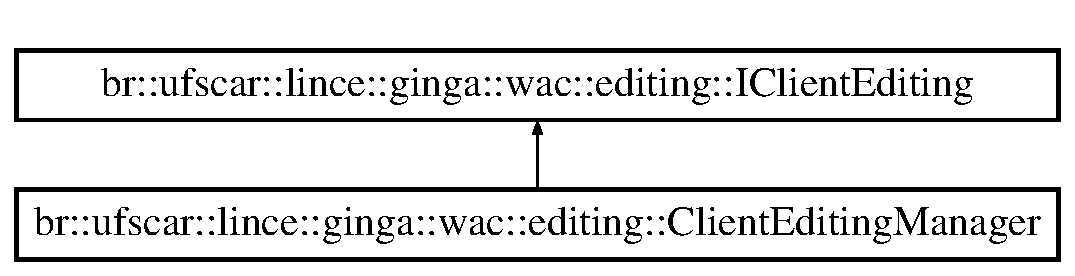
\includegraphics[height=2cm]{classbr_1_1ufscar_1_1lince_1_1ginga_1_1wac_1_1editing_1_1ClientEditingManager}
\end{center}
\end{figure}
\subsection*{Public Member Functions}
\begin{DoxyCompactItemize}
\item 
\hyperlink{classbr_1_1ufscar_1_1lince_1_1ginga_1_1wac_1_1editing_1_1ClientEditingManager_a963d65786d4e563fdb5e091c2aa3215b}{$\sim$ClientEditingManager} ()
\begin{DoxyCompactList}\small\item\em Destrói a instância única de \hyperlink{classbr_1_1ufscar_1_1lince_1_1ginga_1_1wac_1_1editing_1_1ClientEditingManager}{ClientEditingManager}. \item\end{DoxyCompactList}\item 
bool \hyperlink{classbr_1_1ufscar_1_1lince_1_1ginga_1_1wac_1_1editing_1_1ClientEditingManager_a554a556985da2aaa32fe3c705d957705}{addRegion} (string regionId, LayoutRegion $\ast$layoutRegion)
\begin{DoxyCompactList}\small\item\em Adiciona uma Região na Versão Cliente do Documento NCL em execução. \item\end{DoxyCompactList}\item 
bool \hyperlink{classbr_1_1ufscar_1_1lince_1_1ginga_1_1wac_1_1editing_1_1ClientEditingManager_a4f4a856d51b586312be91b376ec0d8f3}{addRegion} (string regionId, string xml)
\begin{DoxyCompactList}\small\item\em Adiciona uma Região na Versão Cliente do Documento NCL em execução. \item\end{DoxyCompactList}\item 
bool \hyperlink{classbr_1_1ufscar_1_1lince_1_1ginga_1_1wac_1_1editing_1_1ClientEditingManager_a21f7109da6d0eb0b54629547513ff69e}{addRule} (Rule $\ast$rule)
\begin{DoxyCompactList}\small\item\em Adiciona uma Regra na Versão Cliente do Documento NCL em execução. \item\end{DoxyCompactList}\item 
bool \hyperlink{classbr_1_1ufscar_1_1lince_1_1ginga_1_1wac_1_1editing_1_1ClientEditingManager_abbf0ba0c717c55996fac349a88f78b6f}{addRule} (string xml)
\begin{DoxyCompactList}\small\item\em Adiciona uma Regra na Versão Cliente do Documento NCL em execução. \item\end{DoxyCompactList}\item 
bool \hyperlink{classbr_1_1ufscar_1_1lince_1_1ginga_1_1wac_1_1editing_1_1ClientEditingManager_a5b363245776a5a71bd3c7628dcf91f7e}{removeRule} (string ruleId)
\begin{DoxyCompactList}\small\item\em Remove uma regra da Versão Cliente do Documento NCL em execução. \item\end{DoxyCompactList}\item 
bool \hyperlink{classbr_1_1ufscar_1_1lince_1_1ginga_1_1wac_1_1editing_1_1ClientEditingManager_af872bea61e20e96b7ef968e24627d8c7}{addTransition} (Transition $\ast$transition)
\begin{DoxyCompactList}\small\item\em Adiciona uma transição na Versão Cliente do Documento NCL em execução. \item\end{DoxyCompactList}\item 
bool \hyperlink{classbr_1_1ufscar_1_1lince_1_1ginga_1_1wac_1_1editing_1_1ClientEditingManager_a474cdd2a429ab96cb5376264ff38fa31}{addTransition} (string xml)
\begin{DoxyCompactList}\small\item\em Adiciona uma transição na Versão Cliente do Documento NCL em execução. \item\end{DoxyCompactList}\item 
bool \hyperlink{classbr_1_1ufscar_1_1lince_1_1ginga_1_1wac_1_1editing_1_1ClientEditingManager_a6aebcca439720cc2c9b69d6b7b5c45c7}{removeTransition} (string transitionId)
\begin{DoxyCompactList}\small\item\em Remove uma transição da Versão Cliente do Documento NCL em execução. \item\end{DoxyCompactList}\item 
bool \hyperlink{classbr_1_1ufscar_1_1lince_1_1ginga_1_1wac_1_1editing_1_1ClientEditingManager_afbc2f133a39eff4008bba3817f8c76a1}{addConnector} (Connector $\ast$connector)
\begin{DoxyCompactList}\small\item\em Adiciona um Conector na Versão Cliente do Documento NCL em execução. \item\end{DoxyCompactList}\item 
bool \hyperlink{classbr_1_1ufscar_1_1lince_1_1ginga_1_1wac_1_1editing_1_1ClientEditingManager_a62f5c2e221cba63f7a47c3a8ce1d154f}{addConnector} (string xml)
\begin{DoxyCompactList}\small\item\em Adiciona um Conector na Versão Cliente do Documento NCL em execução. \item\end{DoxyCompactList}\item 
bool \hyperlink{classbr_1_1ufscar_1_1lince_1_1ginga_1_1wac_1_1editing_1_1ClientEditingManager_a5b6ddc8a6259b07eae8f2c2f03dcdfaa}{removeConnector} (string connectorId)
\begin{DoxyCompactList}\small\item\em Remove um conector da Versão Cliente do Documento NCL em execução. \item\end{DoxyCompactList}\item 
bool \hyperlink{classbr_1_1ufscar_1_1lince_1_1ginga_1_1wac_1_1editing_1_1ClientEditingManager_ad43d65396682df3c57e131e5531e7e4d}{addDescriptor} (GenericDescriptor $\ast$descriptor)
\begin{DoxyCompactList}\small\item\em Adiciona um Descritor na Versão Cliente do Documento NCL em execução. \item\end{DoxyCompactList}\item 
bool \hyperlink{classbr_1_1ufscar_1_1lince_1_1ginga_1_1wac_1_1editing_1_1ClientEditingManager_ab6fd5b9535b8d6e377aab7b7af4c2902}{addDescriptor} (string xml)
\begin{DoxyCompactList}\small\item\em Adiciona um Descritor na Versão Cliente do Documento NCL em execução. \item\end{DoxyCompactList}\item 
bool \hyperlink{classbr_1_1ufscar_1_1lince_1_1ginga_1_1wac_1_1editing_1_1ClientEditingManager_a9b25cb3580c52ddb8147ede64ec53077}{removeDescriptor} (string descriptorId)
\begin{DoxyCompactList}\small\item\em Remove um descritor da Versão Cliente do Documento NCL em execução. \item\end{DoxyCompactList}\item 
bool \hyperlink{classbr_1_1ufscar_1_1lince_1_1ginga_1_1wac_1_1editing_1_1ClientEditingManager_a8e27f52402bb58a3e49d63b28652b2b9}{addNode} (string compositeId, Node $\ast$node)
\begin{DoxyCompactList}\small\item\em Adiciona um Nó à Versão Cliente do Documento NCL em execução. \item\end{DoxyCompactList}\item 
bool \hyperlink{classbr_1_1ufscar_1_1lince_1_1ginga_1_1wac_1_1editing_1_1ClientEditingManager_aa7ddb3cd14fd26fe7e4edf8b3024fdb7}{addNode} (string compositeId, string xml)
\begin{DoxyCompactList}\small\item\em Adiciona um Nó à Versão Cliente do Documento NCL em execução. \item\end{DoxyCompactList}\item 
bool \hyperlink{classbr_1_1ufscar_1_1lince_1_1ginga_1_1wac_1_1editing_1_1ClientEditingManager_a7e6eaecc65141d2660bdb1b1c33c421f}{addInterface} (string nodeId, InterfacePoint $\ast$interface)
\begin{DoxyCompactList}\small\item\em Adiciona uma Interface à Versão Cliente do Documento NCL em execução. \item\end{DoxyCompactList}\item 
bool \hyperlink{classbr_1_1ufscar_1_1lince_1_1ginga_1_1wac_1_1editing_1_1ClientEditingManager_a1565a7f4347ad519fc405455c603fb3c}{addInterface} (string nodeId, string xml)
\begin{DoxyCompactList}\small\item\em Adiciona uma Interface à Versão Cliente do Documento NCL em execução. \item\end{DoxyCompactList}\item 
bool \hyperlink{classbr_1_1ufscar_1_1lince_1_1ginga_1_1wac_1_1editing_1_1ClientEditingManager_a23d60db841bf10edd6266de52613b9b2}{removeInterface} (string nodeId, string interfaceId)
\begin{DoxyCompactList}\small\item\em Remove uma interface da Versão Cliente do Documento NCL em execução. \item\end{DoxyCompactList}\item 
bool \hyperlink{classbr_1_1ufscar_1_1lince_1_1ginga_1_1wac_1_1editing_1_1ClientEditingManager_a53cb5ddc1e425c7f03c7aacff140223c}{addLink} (string compositeId, Link $\ast$link)
\begin{DoxyCompactList}\small\item\em Adiciona um elo à Versão Cliente do Documento NCL em execução. \item\end{DoxyCompactList}\item 
bool \hyperlink{classbr_1_1ufscar_1_1lince_1_1ginga_1_1wac_1_1editing_1_1ClientEditingManager_a88c07d75d150d08724ec077fa54f2aeb}{addLink} (string compositeId, string xml)
\begin{DoxyCompactList}\small\item\em Adiciona um elo à Versão Cliente do Documento NCL em execução. \item\end{DoxyCompactList}\item 
bool \hyperlink{classbr_1_1ufscar_1_1lince_1_1ginga_1_1wac_1_1editing_1_1ClientEditingManager_a11e5f1029545aa4c0435094cc59477cb}{removeLink} (string compositeId, string linkId)
\begin{DoxyCompactList}\small\item\em Remove um elo da Versão Cliente do Documento NCL em execução. \item\end{DoxyCompactList}\item 
NclDocument $\ast$ \hyperlink{classbr_1_1ufscar_1_1lince_1_1ginga_1_1wac_1_1editing_1_1ClientEditingManager_a49b1b969381d54583a4c0ae61756ba7b}{getCurrentDocument} ()
\begin{DoxyCompactList}\small\item\em Retorno a instância que representa o documento NCl que esta sendo apresentado. \item\end{DoxyCompactList}\item 
bool \hyperlink{classbr_1_1ufscar_1_1lince_1_1ginga_1_1wac_1_1editing_1_1ClientEditingManager_a7094577521bafedebcd7edafe753774f}{undoLastEditing} (int n=1)
\begin{DoxyCompactList}\small\item\em Permite desfazer as ultimas edições realizadas por aplicações do cliente. \item\end{DoxyCompactList}\item 
void \hyperlink{classbr_1_1ufscar_1_1lince_1_1ginga_1_1wac_1_1editing_1_1ClientEditingManager_af64ee7af65344bf8c0eba75c33a9e29c}{setCurrentDocument} (NclDocument $\ast$nclDocument)
\begin{DoxyCompactList}\small\item\em Método utilizado para setar o documento ncl atualmente em execução. \item\end{DoxyCompactList}\item 
void \hyperlink{classbr_1_1ufscar_1_1lince_1_1ginga_1_1wac_1_1editing_1_1ClientEditingManager_a6a57699073fe086e75d16ffd96a5bfc3}{setClientPrivateBaseId} (string id)
\begin{DoxyCompactList}\small\item\em Seta o nome da base privada do cliente. \item\end{DoxyCompactList}\item 
void \hyperlink{classbr_1_1ufscar_1_1lince_1_1ginga_1_1wac_1_1editing_1_1ClientEditingManager_ae80834b5a0aa0ffdfb399a85f92b9bd5}{setBroadcasterPrivateBaseId} (string id)
\begin{DoxyCompactList}\small\item\em Seta o nome da base privada da emissora. \item\end{DoxyCompactList}\item 
void \hyperlink{classbr_1_1ufscar_1_1lince_1_1ginga_1_1wac_1_1editing_1_1ClientEditingManager_a07b41ca3cb59e493972d73c8f8e724b8}{setIFormatterAdpater} (\hyperlink{classbr_1_1ufscar_1_1lince_1_1ginga_1_1wac_1_1editing_1_1IFormatterAdapter}{IFormatterAdapter} $\ast$\hyperlink{classbr_1_1ufscar_1_1lince_1_1ginga_1_1wac_1_1editing_1_1ClientEditingManager_a49d8d70cee155e1d15c5da2cbb107777}{formatter})
\begin{DoxyCompactList}\small\item\em Seta a instância do formatter que irá receber os comandos de edição ao vivo. \item\end{DoxyCompactList}\item 
bool \hyperlink{classbr_1_1ufscar_1_1lince_1_1ginga_1_1wac_1_1editing_1_1ClientEditingManager_a968a7252444aa05bb471f47e4c554d19}{saveCurrentFile} (string fileName)
\begin{DoxyCompactList}\small\item\em Salva o Versão Cliente do documento NCL atualmente em execução em um arquivo. \item\end{DoxyCompactList}\item 
string \hyperlink{classbr_1_1ufscar_1_1lince_1_1ginga_1_1wac_1_1editing_1_1ClientEditingManager_aa305ed84ccf3c46501623df103d7a7e0}{getCurrentDocumentPath} ()
\begin{DoxyCompactList}\small\item\em Retorna o caminho do documento NCL atual. \item\end{DoxyCompactList}\end{DoxyCompactItemize}
\subsection*{Static Public Member Functions}
\begin{DoxyCompactItemize}
\item 
static \hyperlink{classbr_1_1ufscar_1_1lince_1_1ginga_1_1wac_1_1editing_1_1ClientEditingManager}{ClientEditingManager} $\ast$ \hyperlink{classbr_1_1ufscar_1_1lince_1_1ginga_1_1wac_1_1editing_1_1ClientEditingManager_ad72c33ccec250438af9b2c489634c42d}{getInstance} ()
\begin{DoxyCompactList}\small\item\em Permite acessar a instância única de \hyperlink{classbr_1_1ufscar_1_1lince_1_1ginga_1_1wac_1_1editing_1_1ClientEditingManager}{ClientEditingManager}. \item\end{DoxyCompactList}\end{DoxyCompactItemize}
\subsection*{Static Public Attributes}
\begin{DoxyCompactItemize}
\item 
static const string \hyperlink{classbr_1_1ufscar_1_1lince_1_1ginga_1_1wac_1_1editing_1_1ClientEditingManager_ad67459adf66064e713ba4fbf1870ce26}{CLIENT\_\-LINK\_\-PREFIX}
\begin{DoxyCompactList}\small\item\em Prefixo anexado aos identificadores das entidades NCL adicionadas pelo cliente. \item\end{DoxyCompactList}\end{DoxyCompactItemize}
\subsection*{Protected Attributes}
\begin{DoxyCompactItemize}
\item 
\hyperlink{classbr_1_1ufscar_1_1lince_1_1ginga_1_1wac_1_1editing_1_1IFormatterAdapter}{IFormatterAdapter} $\ast$ \hyperlink{classbr_1_1ufscar_1_1lince_1_1ginga_1_1wac_1_1editing_1_1ClientEditingManager_a49d8d70cee155e1d15c5da2cbb107777}{formatter}
\begin{DoxyCompactList}\small\item\em Interface utilizada para comunicação com o Formatter do módulo Formatter. \item\end{DoxyCompactList}\item 
list$<$ \hyperlink{classbr_1_1ufscar_1_1lince_1_1ginga_1_1wac_1_1editing_1_1EditingCommand}{EditingCommand} $\ast$ $>$ $\ast$ \hyperlink{classbr_1_1ufscar_1_1lince_1_1ginga_1_1wac_1_1editing_1_1ClientEditingManager_aa89f63aad52acdd1fc2502ebe6193be8}{editingCommands}
\begin{DoxyCompactList}\small\item\em Lista que contém todas os comandos de edição enviados por aplicações cliente. \item\end{DoxyCompactList}\item 
map$<$ string, \hyperlink{classbr_1_1ufscar_1_1lince_1_1ginga_1_1wac_1_1editing_1_1EditingCommand}{EditingCommand} $\ast$ $>$ $\ast$ \hyperlink{classbr_1_1ufscar_1_1lince_1_1ginga_1_1wac_1_1editing_1_1ClientEditingManager_a01857fae3b654789d6a6eb665bf9e058}{mapCommands}
\begin{DoxyCompactList}\small\item\em Mapa que relaciona os comandos de edições com as Ids das entidades NCL adicionadas ou removidas. \item\end{DoxyCompactList}\item 
NclDocument $\ast$ \hyperlink{classbr_1_1ufscar_1_1lince_1_1ginga_1_1wac_1_1editing_1_1ClientEditingManager_a9a5b80d7a04837b9796f3ef87972d99a}{currentDocument}
\begin{DoxyCompactList}\small\item\em Instância do documento NCL atualmente em execução. \item\end{DoxyCompactList}\item 
string \hyperlink{classbr_1_1ufscar_1_1lince_1_1ginga_1_1wac_1_1editing_1_1ClientEditingManager_a7610c9f79a41fb3cd819cffdd8c3d576}{clientPrivateBaseId}
\begin{DoxyCompactList}\small\item\em Nome da Base Privada dos documentos do Cliente. \item\end{DoxyCompactList}\item 
string \hyperlink{classbr_1_1ufscar_1_1lince_1_1ginga_1_1wac_1_1editing_1_1ClientEditingManager_ae6f42fa31a4a78d07977ee83561ed60d}{broadcasterPrivateBaseId}
\begin{DoxyCompactList}\small\item\em Nome da Base Privada dos documentos da emissora. \item\end{DoxyCompactList}\item 
string \hyperlink{classbr_1_1ufscar_1_1lince_1_1ginga_1_1wac_1_1editing_1_1ClientEditingManager_a259109a4e6e19ad1cc8b193f99140c7d}{documentPath}
\begin{DoxyCompactList}\small\item\em Caminho onde esta gravado o documento NCL atualmente em execução. \item\end{DoxyCompactList}\end{DoxyCompactItemize}
\subsection*{Static Protected Attributes}
\begin{DoxyCompactItemize}
\item 
static \hyperlink{classbr_1_1ufscar_1_1lince_1_1ginga_1_1wac_1_1editing_1_1ClientEditingManager}{ClientEditingManager} $\ast$ \hyperlink{classbr_1_1ufscar_1_1lince_1_1ginga_1_1wac_1_1editing_1_1ClientEditingManager_a127cda95b090ee9d020494d2c958be62}{\_\-instance}
\begin{DoxyCompactList}\small\item\em Instância única de \hyperlink{classbr_1_1ufscar_1_1lince_1_1ginga_1_1wac_1_1editing_1_1ClientEditingManager}{ClientEditingManager}. \item\end{DoxyCompactList}\end{DoxyCompactItemize}


\subsection{Detailed Description}
Permite a aplicações desenvolvidas pelo usuário realizar anotações e edições ao vivo em um documento NCL Esta classe basicamente facilita a criação de aplicações de anotação e edição ao vivo do lado cliente, pois faz parte das tarefas necessárias para aplicações deste tipo, além de permitir retroceder de alterações erroneas e fazer um log das alterações. 

\subsection{Constructor \& Destructor Documentation}
\hypertarget{classbr_1_1ufscar_1_1lince_1_1ginga_1_1wac_1_1editing_1_1ClientEditingManager_a963d65786d4e563fdb5e091c2aa3215b}{
\index{br::ufscar::lince::ginga::wac::editing::ClientEditingManager@{br::ufscar::lince::ginga::wac::editing::ClientEditingManager}!$\sim$ClientEditingManager@{$\sim$ClientEditingManager}}
\index{$\sim$ClientEditingManager@{$\sim$ClientEditingManager}!br::ufscar::lince::ginga::wac::editing::ClientEditingManager@{br::ufscar::lince::ginga::wac::editing::ClientEditingManager}}
\subsubsection[{$\sim$ClientEditingManager}]{\setlength{\rightskip}{0pt plus 5cm}br::ufscar::lince::ginga::wac::editing::ClientEditingManager::$\sim$ClientEditingManager ()}}
\label{classbr_1_1ufscar_1_1lince_1_1ginga_1_1wac_1_1editing_1_1ClientEditingManager_a963d65786d4e563fdb5e091c2aa3215b}


Destrói a instância única de \hyperlink{classbr_1_1ufscar_1_1lince_1_1ginga_1_1wac_1_1editing_1_1ClientEditingManager}{ClientEditingManager}. 



\subsection{Member Function Documentation}
\hypertarget{classbr_1_1ufscar_1_1lince_1_1ginga_1_1wac_1_1editing_1_1ClientEditingManager_a62f5c2e221cba63f7a47c3a8ce1d154f}{
\index{br::ufscar::lince::ginga::wac::editing::ClientEditingManager@{br::ufscar::lince::ginga::wac::editing::ClientEditingManager}!addConnector@{addConnector}}
\index{addConnector@{addConnector}!br::ufscar::lince::ginga::wac::editing::ClientEditingManager@{br::ufscar::lince::ginga::wac::editing::ClientEditingManager}}
\subsubsection[{addConnector}]{\setlength{\rightskip}{0pt plus 5cm}bool br::ufscar::lince::ginga::wac::editing::ClientEditingManager::addConnector (string {\em xml})\hspace{0.3cm}{\ttfamily  \mbox{[}virtual\mbox{]}}}}
\label{classbr_1_1ufscar_1_1lince_1_1ginga_1_1wac_1_1editing_1_1ClientEditingManager_a62f5c2e221cba63f7a47c3a8ce1d154f}


Adiciona um Conector na Versão Cliente do Documento NCL em execução. 


\begin{DoxyParams}{Parameters}
\item[{\em xml}]Código xml do conector que será adiconado. \end{DoxyParams}
\begin{DoxyReturn}{Returns}
True se o conector foi adicionado; False caso contrário. 
\end{DoxyReturn}


Implements \hyperlink{classbr_1_1ufscar_1_1lince_1_1ginga_1_1wac_1_1editing_1_1IClientEditing_a531eb37bc22963dcb2feeed0e07591bd}{br::ufscar::lince::ginga::wac::editing::IClientEditing}.

\hypertarget{classbr_1_1ufscar_1_1lince_1_1ginga_1_1wac_1_1editing_1_1ClientEditingManager_afbc2f133a39eff4008bba3817f8c76a1}{
\index{br::ufscar::lince::ginga::wac::editing::ClientEditingManager@{br::ufscar::lince::ginga::wac::editing::ClientEditingManager}!addConnector@{addConnector}}
\index{addConnector@{addConnector}!br::ufscar::lince::ginga::wac::editing::ClientEditingManager@{br::ufscar::lince::ginga::wac::editing::ClientEditingManager}}
\subsubsection[{addConnector}]{\setlength{\rightskip}{0pt plus 5cm}bool br::ufscar::lince::ginga::wac::editing::ClientEditingManager::addConnector (Connector $\ast$ {\em connector})\hspace{0.3cm}{\ttfamily  \mbox{[}virtual\mbox{]}}}}
\label{classbr_1_1ufscar_1_1lince_1_1ginga_1_1wac_1_1editing_1_1ClientEditingManager_afbc2f133a39eff4008bba3817f8c76a1}


Adiciona um Conector na Versão Cliente do Documento NCL em execução. 


\begin{DoxyParams}{Parameters}
\item[{\em connector}]Instância que representa o conector que será adiconado. \end{DoxyParams}
\begin{DoxyReturn}{Returns}
True se o conector foi adicionado; False caso contrário. 
\end{DoxyReturn}


Implements \hyperlink{classbr_1_1ufscar_1_1lince_1_1ginga_1_1wac_1_1editing_1_1IClientEditing_ac3ce7f9f55bc61cb7166b741a73e77d9}{br::ufscar::lince::ginga::wac::editing::IClientEditing}.

\hypertarget{classbr_1_1ufscar_1_1lince_1_1ginga_1_1wac_1_1editing_1_1ClientEditingManager_ab6fd5b9535b8d6e377aab7b7af4c2902}{
\index{br::ufscar::lince::ginga::wac::editing::ClientEditingManager@{br::ufscar::lince::ginga::wac::editing::ClientEditingManager}!addDescriptor@{addDescriptor}}
\index{addDescriptor@{addDescriptor}!br::ufscar::lince::ginga::wac::editing::ClientEditingManager@{br::ufscar::lince::ginga::wac::editing::ClientEditingManager}}
\subsubsection[{addDescriptor}]{\setlength{\rightskip}{0pt plus 5cm}bool br::ufscar::lince::ginga::wac::editing::ClientEditingManager::addDescriptor (string {\em xml})\hspace{0.3cm}{\ttfamily  \mbox{[}virtual\mbox{]}}}}
\label{classbr_1_1ufscar_1_1lince_1_1ginga_1_1wac_1_1editing_1_1ClientEditingManager_ab6fd5b9535b8d6e377aab7b7af4c2902}


Adiciona um Descritor na Versão Cliente do Documento NCL em execução. 


\begin{DoxyParams}{Parameters}
\item[{\em xml}]Código xml do Descritor que será adiconado. \end{DoxyParams}
\begin{DoxyReturn}{Returns}
True se o Descritor foi adicionado; False caso contrário. 
\end{DoxyReturn}


Implements \hyperlink{classbr_1_1ufscar_1_1lince_1_1ginga_1_1wac_1_1editing_1_1IClientEditing_af7aa3b95abda814fbf7cadbd277dc2c1}{br::ufscar::lince::ginga::wac::editing::IClientEditing}.

\hypertarget{classbr_1_1ufscar_1_1lince_1_1ginga_1_1wac_1_1editing_1_1ClientEditingManager_ad43d65396682df3c57e131e5531e7e4d}{
\index{br::ufscar::lince::ginga::wac::editing::ClientEditingManager@{br::ufscar::lince::ginga::wac::editing::ClientEditingManager}!addDescriptor@{addDescriptor}}
\index{addDescriptor@{addDescriptor}!br::ufscar::lince::ginga::wac::editing::ClientEditingManager@{br::ufscar::lince::ginga::wac::editing::ClientEditingManager}}
\subsubsection[{addDescriptor}]{\setlength{\rightskip}{0pt plus 5cm}bool br::ufscar::lince::ginga::wac::editing::ClientEditingManager::addDescriptor (GenericDescriptor $\ast$ {\em descriptor})\hspace{0.3cm}{\ttfamily  \mbox{[}virtual\mbox{]}}}}
\label{classbr_1_1ufscar_1_1lince_1_1ginga_1_1wac_1_1editing_1_1ClientEditingManager_ad43d65396682df3c57e131e5531e7e4d}


Adiciona um Descritor na Versão Cliente do Documento NCL em execução. 


\begin{DoxyParams}{Parameters}
\item[{\em descriptor}]Instância que representa o Descritor que será adiconado. \end{DoxyParams}
\begin{DoxyReturn}{Returns}
True se o Descritor foi adicionado; False caso contrário. 
\end{DoxyReturn}


Implements \hyperlink{classbr_1_1ufscar_1_1lince_1_1ginga_1_1wac_1_1editing_1_1IClientEditing_a8fb8afeaa96087d789b6b0efd9571853}{br::ufscar::lince::ginga::wac::editing::IClientEditing}.

\hypertarget{classbr_1_1ufscar_1_1lince_1_1ginga_1_1wac_1_1editing_1_1ClientEditingManager_a1565a7f4347ad519fc405455c603fb3c}{
\index{br::ufscar::lince::ginga::wac::editing::ClientEditingManager@{br::ufscar::lince::ginga::wac::editing::ClientEditingManager}!addInterface@{addInterface}}
\index{addInterface@{addInterface}!br::ufscar::lince::ginga::wac::editing::ClientEditingManager@{br::ufscar::lince::ginga::wac::editing::ClientEditingManager}}
\subsubsection[{addInterface}]{\setlength{\rightskip}{0pt plus 5cm}bool br::ufscar::lince::ginga::wac::editing::ClientEditingManager::addInterface (string {\em nodeId}, \/  string {\em xml})\hspace{0.3cm}{\ttfamily  \mbox{[}virtual\mbox{]}}}}
\label{classbr_1_1ufscar_1_1lince_1_1ginga_1_1wac_1_1editing_1_1ClientEditingManager_a1565a7f4347ad519fc405455c603fb3c}


Adiciona uma Interface à Versão Cliente do Documento NCL em execução. 


\begin{DoxyParams}{Parameters}
\item[{\em nodeId}]Idenitificador do nó onde esta nova interface será adicionada. \item[{\em xml}]Código xml da interface que será adiconada. \end{DoxyParams}
\begin{DoxyReturn}{Returns}
True se a interface foi adicionada; False caso contrário. 
\end{DoxyReturn}


Implements \hyperlink{classbr_1_1ufscar_1_1lince_1_1ginga_1_1wac_1_1editing_1_1IClientEditing_af60b6d775c412012b85a219311bbc4d8}{br::ufscar::lince::ginga::wac::editing::IClientEditing}.

\hypertarget{classbr_1_1ufscar_1_1lince_1_1ginga_1_1wac_1_1editing_1_1ClientEditingManager_a7e6eaecc65141d2660bdb1b1c33c421f}{
\index{br::ufscar::lince::ginga::wac::editing::ClientEditingManager@{br::ufscar::lince::ginga::wac::editing::ClientEditingManager}!addInterface@{addInterface}}
\index{addInterface@{addInterface}!br::ufscar::lince::ginga::wac::editing::ClientEditingManager@{br::ufscar::lince::ginga::wac::editing::ClientEditingManager}}
\subsubsection[{addInterface}]{\setlength{\rightskip}{0pt plus 5cm}bool br::ufscar::lince::ginga::wac::editing::ClientEditingManager::addInterface (string {\em nodeId}, \/  InterfacePoint $\ast$ {\em interface})\hspace{0.3cm}{\ttfamily  \mbox{[}virtual\mbox{]}}}}
\label{classbr_1_1ufscar_1_1lince_1_1ginga_1_1wac_1_1editing_1_1ClientEditingManager_a7e6eaecc65141d2660bdb1b1c33c421f}


Adiciona uma Interface à Versão Cliente do Documento NCL em execução. 


\begin{DoxyParams}{Parameters}
\item[{\em nodeId}]Idenitificador do nó onde esta nova interface será adicionada. \item[{\em interface}]Instância que representa a interface que será adiconada. \end{DoxyParams}
\begin{DoxyReturn}{Returns}
True se a interface foi adicionada; False caso contrário. 
\end{DoxyReturn}


Implements \hyperlink{classbr_1_1ufscar_1_1lince_1_1ginga_1_1wac_1_1editing_1_1IClientEditing_a7a733528927ed22d232ae58e0539b1eb}{br::ufscar::lince::ginga::wac::editing::IClientEditing}.

\hypertarget{classbr_1_1ufscar_1_1lince_1_1ginga_1_1wac_1_1editing_1_1ClientEditingManager_a88c07d75d150d08724ec077fa54f2aeb}{
\index{br::ufscar::lince::ginga::wac::editing::ClientEditingManager@{br::ufscar::lince::ginga::wac::editing::ClientEditingManager}!addLink@{addLink}}
\index{addLink@{addLink}!br::ufscar::lince::ginga::wac::editing::ClientEditingManager@{br::ufscar::lince::ginga::wac::editing::ClientEditingManager}}
\subsubsection[{addLink}]{\setlength{\rightskip}{0pt plus 5cm}bool br::ufscar::lince::ginga::wac::editing::ClientEditingManager::addLink (string {\em compositeId}, \/  string {\em xml})\hspace{0.3cm}{\ttfamily  \mbox{[}virtual\mbox{]}}}}
\label{classbr_1_1ufscar_1_1lince_1_1ginga_1_1wac_1_1editing_1_1ClientEditingManager_a88c07d75d150d08724ec077fa54f2aeb}


Adiciona um elo à Versão Cliente do Documento NCL em execução. 


\begin{DoxyParams}{Parameters}
\item[{\em compositeId}]Idenitificador do nó de contexto onde este novo elo será adicionado. \item[{\em xml}]Código xml do elo que será adiconado. \end{DoxyParams}
\begin{DoxyReturn}{Returns}
True se o elo foi adicionado; False caso contrário. 
\end{DoxyReturn}


Implements \hyperlink{classbr_1_1ufscar_1_1lince_1_1ginga_1_1wac_1_1editing_1_1IClientEditing_aa9d2c5d6522cc5428abc2a3231299b74}{br::ufscar::lince::ginga::wac::editing::IClientEditing}.

\hypertarget{classbr_1_1ufscar_1_1lince_1_1ginga_1_1wac_1_1editing_1_1ClientEditingManager_a53cb5ddc1e425c7f03c7aacff140223c}{
\index{br::ufscar::lince::ginga::wac::editing::ClientEditingManager@{br::ufscar::lince::ginga::wac::editing::ClientEditingManager}!addLink@{addLink}}
\index{addLink@{addLink}!br::ufscar::lince::ginga::wac::editing::ClientEditingManager@{br::ufscar::lince::ginga::wac::editing::ClientEditingManager}}
\subsubsection[{addLink}]{\setlength{\rightskip}{0pt plus 5cm}bool br::ufscar::lince::ginga::wac::editing::ClientEditingManager::addLink (string {\em compositeId}, \/  Link $\ast$ {\em link})\hspace{0.3cm}{\ttfamily  \mbox{[}virtual\mbox{]}}}}
\label{classbr_1_1ufscar_1_1lince_1_1ginga_1_1wac_1_1editing_1_1ClientEditingManager_a53cb5ddc1e425c7f03c7aacff140223c}


Adiciona um elo à Versão Cliente do Documento NCL em execução. 


\begin{DoxyParams}{Parameters}
\item[{\em compositeId}]Idenitificador do nó de contexto onde este novo elo será adicionado. \item[{\em link}]Instancia que representa o elo que será adiconado. \end{DoxyParams}
\begin{DoxyReturn}{Returns}
True se o elo foi adicionado; False caso contrário. 
\end{DoxyReturn}


Implements \hyperlink{classbr_1_1ufscar_1_1lince_1_1ginga_1_1wac_1_1editing_1_1IClientEditing_a74829dbd18d200ef2522a0e228e20a10}{br::ufscar::lince::ginga::wac::editing::IClientEditing}.

\hypertarget{classbr_1_1ufscar_1_1lince_1_1ginga_1_1wac_1_1editing_1_1ClientEditingManager_aa7ddb3cd14fd26fe7e4edf8b3024fdb7}{
\index{br::ufscar::lince::ginga::wac::editing::ClientEditingManager@{br::ufscar::lince::ginga::wac::editing::ClientEditingManager}!addNode@{addNode}}
\index{addNode@{addNode}!br::ufscar::lince::ginga::wac::editing::ClientEditingManager@{br::ufscar::lince::ginga::wac::editing::ClientEditingManager}}
\subsubsection[{addNode}]{\setlength{\rightskip}{0pt plus 5cm}bool br::ufscar::lince::ginga::wac::editing::ClientEditingManager::addNode (string {\em compositeId}, \/  string {\em xml})\hspace{0.3cm}{\ttfamily  \mbox{[}virtual\mbox{]}}}}
\label{classbr_1_1ufscar_1_1lince_1_1ginga_1_1wac_1_1editing_1_1ClientEditingManager_aa7ddb3cd14fd26fe7e4edf8b3024fdb7}


Adiciona um Nó à Versão Cliente do Documento NCL em execução. 


\begin{DoxyParams}{Parameters}
\item[{\em compositeId}]Idenitificador do nó onde este novo nó será adicionado. \item[{\em xml}]Código xml do nó que será adiconado. \end{DoxyParams}
\begin{DoxyReturn}{Returns}
True se o nó foi adicionado; False caso contrário. 
\end{DoxyReturn}


Implements \hyperlink{classbr_1_1ufscar_1_1lince_1_1ginga_1_1wac_1_1editing_1_1IClientEditing_ad101947701dbbef3d365d92ae385ec46}{br::ufscar::lince::ginga::wac::editing::IClientEditing}.

\hypertarget{classbr_1_1ufscar_1_1lince_1_1ginga_1_1wac_1_1editing_1_1ClientEditingManager_a8e27f52402bb58a3e49d63b28652b2b9}{
\index{br::ufscar::lince::ginga::wac::editing::ClientEditingManager@{br::ufscar::lince::ginga::wac::editing::ClientEditingManager}!addNode@{addNode}}
\index{addNode@{addNode}!br::ufscar::lince::ginga::wac::editing::ClientEditingManager@{br::ufscar::lince::ginga::wac::editing::ClientEditingManager}}
\subsubsection[{addNode}]{\setlength{\rightskip}{0pt plus 5cm}bool br::ufscar::lince::ginga::wac::editing::ClientEditingManager::addNode (string {\em compositeId}, \/  Node $\ast$ {\em node})\hspace{0.3cm}{\ttfamily  \mbox{[}virtual\mbox{]}}}}
\label{classbr_1_1ufscar_1_1lince_1_1ginga_1_1wac_1_1editing_1_1ClientEditingManager_a8e27f52402bb58a3e49d63b28652b2b9}


Adiciona um Nó à Versão Cliente do Documento NCL em execução. 


\begin{DoxyParams}{Parameters}
\item[{\em compositeId}]Idenitificador do nó onde este novo nó será adicionado. \item[{\em node}]Instância que representa o nó que será adiconado. \end{DoxyParams}
\begin{DoxyReturn}{Returns}
True se o nó foi adicionado; False caso contrário. 
\end{DoxyReturn}


Implements \hyperlink{classbr_1_1ufscar_1_1lince_1_1ginga_1_1wac_1_1editing_1_1IClientEditing_ad8662a9f157872a4cbe7ed0da9baf3fb}{br::ufscar::lince::ginga::wac::editing::IClientEditing}.

\hypertarget{classbr_1_1ufscar_1_1lince_1_1ginga_1_1wac_1_1editing_1_1ClientEditingManager_a4f4a856d51b586312be91b376ec0d8f3}{
\index{br::ufscar::lince::ginga::wac::editing::ClientEditingManager@{br::ufscar::lince::ginga::wac::editing::ClientEditingManager}!addRegion@{addRegion}}
\index{addRegion@{addRegion}!br::ufscar::lince::ginga::wac::editing::ClientEditingManager@{br::ufscar::lince::ginga::wac::editing::ClientEditingManager}}
\subsubsection[{addRegion}]{\setlength{\rightskip}{0pt plus 5cm}bool br::ufscar::lince::ginga::wac::editing::ClientEditingManager::addRegion (string {\em regionId}, \/  string {\em xml})\hspace{0.3cm}{\ttfamily  \mbox{[}virtual\mbox{]}}}}
\label{classbr_1_1ufscar_1_1lince_1_1ginga_1_1wac_1_1editing_1_1ClientEditingManager_a4f4a856d51b586312be91b376ec0d8f3}


Adiciona uma Região na Versão Cliente do Documento NCL em execução. 


\begin{DoxyParams}{Parameters}
\item[{\em regionId}]Identificador da Região onde a nova Região será adiconada. \item[{\em xml}]Código xml da Região que será adiconada. \end{DoxyParams}
\begin{DoxyReturn}{Returns}
True se a região foi adicionada; False caso contrário. 
\end{DoxyReturn}


Implements \hyperlink{classbr_1_1ufscar_1_1lince_1_1ginga_1_1wac_1_1editing_1_1IClientEditing_afaa30256c70e59a36820317d203869fc}{br::ufscar::lince::ginga::wac::editing::IClientEditing}.

\hypertarget{classbr_1_1ufscar_1_1lince_1_1ginga_1_1wac_1_1editing_1_1ClientEditingManager_a554a556985da2aaa32fe3c705d957705}{
\index{br::ufscar::lince::ginga::wac::editing::ClientEditingManager@{br::ufscar::lince::ginga::wac::editing::ClientEditingManager}!addRegion@{addRegion}}
\index{addRegion@{addRegion}!br::ufscar::lince::ginga::wac::editing::ClientEditingManager@{br::ufscar::lince::ginga::wac::editing::ClientEditingManager}}
\subsubsection[{addRegion}]{\setlength{\rightskip}{0pt plus 5cm}bool br::ufscar::lince::ginga::wac::editing::ClientEditingManager::addRegion (string {\em regionId}, \/  LayoutRegion $\ast$ {\em layoutRegion})\hspace{0.3cm}{\ttfamily  \mbox{[}virtual\mbox{]}}}}
\label{classbr_1_1ufscar_1_1lince_1_1ginga_1_1wac_1_1editing_1_1ClientEditingManager_a554a556985da2aaa32fe3c705d957705}


Adiciona uma Região na Versão Cliente do Documento NCL em execução. 


\begin{DoxyParams}{Parameters}
\item[{\em regionId}]Identificador da Região onde a nova Região será adiconada. \item[{\em layoutRegion}]Instância que representa a Região que será adiconada. \end{DoxyParams}
\begin{DoxyReturn}{Returns}
True se a região foi adicionada; False caso contrário. 
\end{DoxyReturn}


Implements \hyperlink{classbr_1_1ufscar_1_1lince_1_1ginga_1_1wac_1_1editing_1_1IClientEditing_a159d8e1b676431ee5439ad932f07a6bd}{br::ufscar::lince::ginga::wac::editing::IClientEditing}.

\hypertarget{classbr_1_1ufscar_1_1lince_1_1ginga_1_1wac_1_1editing_1_1ClientEditingManager_abbf0ba0c717c55996fac349a88f78b6f}{
\index{br::ufscar::lince::ginga::wac::editing::ClientEditingManager@{br::ufscar::lince::ginga::wac::editing::ClientEditingManager}!addRule@{addRule}}
\index{addRule@{addRule}!br::ufscar::lince::ginga::wac::editing::ClientEditingManager@{br::ufscar::lince::ginga::wac::editing::ClientEditingManager}}
\subsubsection[{addRule}]{\setlength{\rightskip}{0pt plus 5cm}bool br::ufscar::lince::ginga::wac::editing::ClientEditingManager::addRule (string {\em xml})\hspace{0.3cm}{\ttfamily  \mbox{[}virtual\mbox{]}}}}
\label{classbr_1_1ufscar_1_1lince_1_1ginga_1_1wac_1_1editing_1_1ClientEditingManager_abbf0ba0c717c55996fac349a88f78b6f}


Adiciona uma Regra na Versão Cliente do Documento NCL em execução. 


\begin{DoxyParams}{Parameters}
\item[{\em xml}]Código xml da Regra que será adiconada. \end{DoxyParams}
\begin{DoxyReturn}{Returns}
True se a regra foi adicionada; False caso contrário. 
\end{DoxyReturn}


Implements \hyperlink{classbr_1_1ufscar_1_1lince_1_1ginga_1_1wac_1_1editing_1_1IClientEditing_a9268c1aa4301692ad9ed3c17e97d5f45}{br::ufscar::lince::ginga::wac::editing::IClientEditing}.

\hypertarget{classbr_1_1ufscar_1_1lince_1_1ginga_1_1wac_1_1editing_1_1ClientEditingManager_a21f7109da6d0eb0b54629547513ff69e}{
\index{br::ufscar::lince::ginga::wac::editing::ClientEditingManager@{br::ufscar::lince::ginga::wac::editing::ClientEditingManager}!addRule@{addRule}}
\index{addRule@{addRule}!br::ufscar::lince::ginga::wac::editing::ClientEditingManager@{br::ufscar::lince::ginga::wac::editing::ClientEditingManager}}
\subsubsection[{addRule}]{\setlength{\rightskip}{0pt plus 5cm}bool br::ufscar::lince::ginga::wac::editing::ClientEditingManager::addRule (Rule $\ast$ {\em rule})\hspace{0.3cm}{\ttfamily  \mbox{[}virtual\mbox{]}}}}
\label{classbr_1_1ufscar_1_1lince_1_1ginga_1_1wac_1_1editing_1_1ClientEditingManager_a21f7109da6d0eb0b54629547513ff69e}


Adiciona uma Regra na Versão Cliente do Documento NCL em execução. 


\begin{DoxyParams}{Parameters}
\item[{\em rule}]Instância que representa a Regra que será adiconada. \end{DoxyParams}
\begin{DoxyReturn}{Returns}
True se a regra foi adicionada; False caso contrário. 
\end{DoxyReturn}


Implements \hyperlink{classbr_1_1ufscar_1_1lince_1_1ginga_1_1wac_1_1editing_1_1IClientEditing_abc156e111b7741a7f55c28b835614178}{br::ufscar::lince::ginga::wac::editing::IClientEditing}.

\hypertarget{classbr_1_1ufscar_1_1lince_1_1ginga_1_1wac_1_1editing_1_1ClientEditingManager_a474cdd2a429ab96cb5376264ff38fa31}{
\index{br::ufscar::lince::ginga::wac::editing::ClientEditingManager@{br::ufscar::lince::ginga::wac::editing::ClientEditingManager}!addTransition@{addTransition}}
\index{addTransition@{addTransition}!br::ufscar::lince::ginga::wac::editing::ClientEditingManager@{br::ufscar::lince::ginga::wac::editing::ClientEditingManager}}
\subsubsection[{addTransition}]{\setlength{\rightskip}{0pt plus 5cm}bool br::ufscar::lince::ginga::wac::editing::ClientEditingManager::addTransition (string {\em xml})\hspace{0.3cm}{\ttfamily  \mbox{[}virtual\mbox{]}}}}
\label{classbr_1_1ufscar_1_1lince_1_1ginga_1_1wac_1_1editing_1_1ClientEditingManager_a474cdd2a429ab96cb5376264ff38fa31}


Adiciona uma transição na Versão Cliente do Documento NCL em execução. 


\begin{DoxyParams}{Parameters}
\item[{\em xml}]Código xml da transição que será adiconada. \end{DoxyParams}
\begin{DoxyReturn}{Returns}
True se a transição foi adicionada; False caso contrário. 
\end{DoxyReturn}


Implements \hyperlink{classbr_1_1ufscar_1_1lince_1_1ginga_1_1wac_1_1editing_1_1IClientEditing_ab485ec1908e00b24e451f138446885af}{br::ufscar::lince::ginga::wac::editing::IClientEditing}.

\hypertarget{classbr_1_1ufscar_1_1lince_1_1ginga_1_1wac_1_1editing_1_1ClientEditingManager_af872bea61e20e96b7ef968e24627d8c7}{
\index{br::ufscar::lince::ginga::wac::editing::ClientEditingManager@{br::ufscar::lince::ginga::wac::editing::ClientEditingManager}!addTransition@{addTransition}}
\index{addTransition@{addTransition}!br::ufscar::lince::ginga::wac::editing::ClientEditingManager@{br::ufscar::lince::ginga::wac::editing::ClientEditingManager}}
\subsubsection[{addTransition}]{\setlength{\rightskip}{0pt plus 5cm}bool br::ufscar::lince::ginga::wac::editing::ClientEditingManager::addTransition (Transition $\ast$ {\em transition})\hspace{0.3cm}{\ttfamily  \mbox{[}virtual\mbox{]}}}}
\label{classbr_1_1ufscar_1_1lince_1_1ginga_1_1wac_1_1editing_1_1ClientEditingManager_af872bea61e20e96b7ef968e24627d8c7}


Adiciona uma transição na Versão Cliente do Documento NCL em execução. 


\begin{DoxyParams}{Parameters}
\item[{\em transition}]Instância que representa a transição que será adiconada. \end{DoxyParams}
\begin{DoxyReturn}{Returns}
True se a transição foi adicionada; False caso contrário. 
\end{DoxyReturn}


Implements \hyperlink{classbr_1_1ufscar_1_1lince_1_1ginga_1_1wac_1_1editing_1_1IClientEditing_a8de701b01f8095605897a83002ea9fb0}{br::ufscar::lince::ginga::wac::editing::IClientEditing}.

\hypertarget{classbr_1_1ufscar_1_1lince_1_1ginga_1_1wac_1_1editing_1_1ClientEditingManager_a49b1b969381d54583a4c0ae61756ba7b}{
\index{br::ufscar::lince::ginga::wac::editing::ClientEditingManager@{br::ufscar::lince::ginga::wac::editing::ClientEditingManager}!getCurrentDocument@{getCurrentDocument}}
\index{getCurrentDocument@{getCurrentDocument}!br::ufscar::lince::ginga::wac::editing::ClientEditingManager@{br::ufscar::lince::ginga::wac::editing::ClientEditingManager}}
\subsubsection[{getCurrentDocument}]{\setlength{\rightskip}{0pt plus 5cm}NclDocument$\ast$ br::ufscar::lince::ginga::wac::editing::ClientEditingManager::getCurrentDocument ()\hspace{0.3cm}{\ttfamily  \mbox{[}virtual\mbox{]}}}}
\label{classbr_1_1ufscar_1_1lince_1_1ginga_1_1wac_1_1editing_1_1ClientEditingManager_a49b1b969381d54583a4c0ae61756ba7b}


Retorno a instância que representa o documento NCl que esta sendo apresentado. 

\begin{DoxyReturn}{Returns}
Documento NCL que está sendo apresentado. 
\end{DoxyReturn}


Implements \hyperlink{classbr_1_1ufscar_1_1lince_1_1ginga_1_1wac_1_1editing_1_1IClientEditing_a72ba6d8611de7d1b8569a5b5d68e4fb9}{br::ufscar::lince::ginga::wac::editing::IClientEditing}.

\hypertarget{classbr_1_1ufscar_1_1lince_1_1ginga_1_1wac_1_1editing_1_1ClientEditingManager_aa305ed84ccf3c46501623df103d7a7e0}{
\index{br::ufscar::lince::ginga::wac::editing::ClientEditingManager@{br::ufscar::lince::ginga::wac::editing::ClientEditingManager}!getCurrentDocumentPath@{getCurrentDocumentPath}}
\index{getCurrentDocumentPath@{getCurrentDocumentPath}!br::ufscar::lince::ginga::wac::editing::ClientEditingManager@{br::ufscar::lince::ginga::wac::editing::ClientEditingManager}}
\subsubsection[{getCurrentDocumentPath}]{\setlength{\rightskip}{0pt plus 5cm}string br::ufscar::lince::ginga::wac::editing::ClientEditingManager::getCurrentDocumentPath ()}}
\label{classbr_1_1ufscar_1_1lince_1_1ginga_1_1wac_1_1editing_1_1ClientEditingManager_aa305ed84ccf3c46501623df103d7a7e0}


Retorna o caminho do documento NCL atual. 

\begin{DoxyReturn}{Returns}
Uma String contendo o caminho do documento NCL atual. 
\end{DoxyReturn}
\hypertarget{classbr_1_1ufscar_1_1lince_1_1ginga_1_1wac_1_1editing_1_1ClientEditingManager_ad72c33ccec250438af9b2c489634c42d}{
\index{br::ufscar::lince::ginga::wac::editing::ClientEditingManager@{br::ufscar::lince::ginga::wac::editing::ClientEditingManager}!getInstance@{getInstance}}
\index{getInstance@{getInstance}!br::ufscar::lince::ginga::wac::editing::ClientEditingManager@{br::ufscar::lince::ginga::wac::editing::ClientEditingManager}}
\subsubsection[{getInstance}]{\setlength{\rightskip}{0pt plus 5cm}static {\bf ClientEditingManager}$\ast$ br::ufscar::lince::ginga::wac::editing::ClientEditingManager::getInstance ()\hspace{0.3cm}{\ttfamily  \mbox{[}static\mbox{]}}}}
\label{classbr_1_1ufscar_1_1lince_1_1ginga_1_1wac_1_1editing_1_1ClientEditingManager_ad72c33ccec250438af9b2c489634c42d}


Permite acessar a instância única de \hyperlink{classbr_1_1ufscar_1_1lince_1_1ginga_1_1wac_1_1editing_1_1ClientEditingManager}{ClientEditingManager}. 

\begin{DoxyReturn}{Returns}
Instância única de \hyperlink{classbr_1_1ufscar_1_1lince_1_1ginga_1_1wac_1_1editing_1_1ClientEditingManager}{ClientEditingManager}. 
\end{DoxyReturn}
\hypertarget{classbr_1_1ufscar_1_1lince_1_1ginga_1_1wac_1_1editing_1_1ClientEditingManager_a5b6ddc8a6259b07eae8f2c2f03dcdfaa}{
\index{br::ufscar::lince::ginga::wac::editing::ClientEditingManager@{br::ufscar::lince::ginga::wac::editing::ClientEditingManager}!removeConnector@{removeConnector}}
\index{removeConnector@{removeConnector}!br::ufscar::lince::ginga::wac::editing::ClientEditingManager@{br::ufscar::lince::ginga::wac::editing::ClientEditingManager}}
\subsubsection[{removeConnector}]{\setlength{\rightskip}{0pt plus 5cm}bool br::ufscar::lince::ginga::wac::editing::ClientEditingManager::removeConnector (string {\em connectorId})\hspace{0.3cm}{\ttfamily  \mbox{[}virtual\mbox{]}}}}
\label{classbr_1_1ufscar_1_1lince_1_1ginga_1_1wac_1_1editing_1_1ClientEditingManager_a5b6ddc8a6259b07eae8f2c2f03dcdfaa}


Remove um conector da Versão Cliente do Documento NCL em execução. 


\begin{DoxyParams}{Parameters}
\item[{\em connectorId}]Identificador do conector que será removido. \end{DoxyParams}
\begin{DoxyReturn}{Returns}
True se o conector for removido; False caso contrário. 
\end{DoxyReturn}


Implements \hyperlink{classbr_1_1ufscar_1_1lince_1_1ginga_1_1wac_1_1editing_1_1IClientEditing_a415ff450552523a495db85c15004c6f9}{br::ufscar::lince::ginga::wac::editing::IClientEditing}.

\hypertarget{classbr_1_1ufscar_1_1lince_1_1ginga_1_1wac_1_1editing_1_1ClientEditingManager_a9b25cb3580c52ddb8147ede64ec53077}{
\index{br::ufscar::lince::ginga::wac::editing::ClientEditingManager@{br::ufscar::lince::ginga::wac::editing::ClientEditingManager}!removeDescriptor@{removeDescriptor}}
\index{removeDescriptor@{removeDescriptor}!br::ufscar::lince::ginga::wac::editing::ClientEditingManager@{br::ufscar::lince::ginga::wac::editing::ClientEditingManager}}
\subsubsection[{removeDescriptor}]{\setlength{\rightskip}{0pt plus 5cm}bool br::ufscar::lince::ginga::wac::editing::ClientEditingManager::removeDescriptor (string {\em descriptorId})\hspace{0.3cm}{\ttfamily  \mbox{[}virtual\mbox{]}}}}
\label{classbr_1_1ufscar_1_1lince_1_1ginga_1_1wac_1_1editing_1_1ClientEditingManager_a9b25cb3580c52ddb8147ede64ec53077}


Remove um descritor da Versão Cliente do Documento NCL em execução. 


\begin{DoxyParams}{Parameters}
\item[{\em descriptorId}]Identificador do descritor que será removido. \end{DoxyParams}
\begin{DoxyReturn}{Returns}
True se o descritor for removido; False caso contrário. 
\end{DoxyReturn}


Implements \hyperlink{classbr_1_1ufscar_1_1lince_1_1ginga_1_1wac_1_1editing_1_1IClientEditing_ad3ae20153844de461ded8a643443dc08}{br::ufscar::lince::ginga::wac::editing::IClientEditing}.

\hypertarget{classbr_1_1ufscar_1_1lince_1_1ginga_1_1wac_1_1editing_1_1ClientEditingManager_a23d60db841bf10edd6266de52613b9b2}{
\index{br::ufscar::lince::ginga::wac::editing::ClientEditingManager@{br::ufscar::lince::ginga::wac::editing::ClientEditingManager}!removeInterface@{removeInterface}}
\index{removeInterface@{removeInterface}!br::ufscar::lince::ginga::wac::editing::ClientEditingManager@{br::ufscar::lince::ginga::wac::editing::ClientEditingManager}}
\subsubsection[{removeInterface}]{\setlength{\rightskip}{0pt plus 5cm}bool br::ufscar::lince::ginga::wac::editing::ClientEditingManager::removeInterface (string {\em nodeId}, \/  string {\em interfaceId})\hspace{0.3cm}{\ttfamily  \mbox{[}virtual\mbox{]}}}}
\label{classbr_1_1ufscar_1_1lince_1_1ginga_1_1wac_1_1editing_1_1ClientEditingManager_a23d60db841bf10edd6266de52613b9b2}


Remove uma interface da Versão Cliente do Documento NCL em execução. 


\begin{DoxyParams}{Parameters}
\item[{\em nodeId}]Idenitificador do nó de onde esta interface será removida. \item[{\em descriptorId}]Identificador do descritor que será removido. \end{DoxyParams}
\begin{DoxyReturn}{Returns}
True se o descritor for removido; False caso contrário. 
\end{DoxyReturn}


Implements \hyperlink{classbr_1_1ufscar_1_1lince_1_1ginga_1_1wac_1_1editing_1_1IClientEditing_abe89650753eccb62bf1772cc0e87d6b7}{br::ufscar::lince::ginga::wac::editing::IClientEditing}.

\hypertarget{classbr_1_1ufscar_1_1lince_1_1ginga_1_1wac_1_1editing_1_1ClientEditingManager_a11e5f1029545aa4c0435094cc59477cb}{
\index{br::ufscar::lince::ginga::wac::editing::ClientEditingManager@{br::ufscar::lince::ginga::wac::editing::ClientEditingManager}!removeLink@{removeLink}}
\index{removeLink@{removeLink}!br::ufscar::lince::ginga::wac::editing::ClientEditingManager@{br::ufscar::lince::ginga::wac::editing::ClientEditingManager}}
\subsubsection[{removeLink}]{\setlength{\rightskip}{0pt plus 5cm}bool br::ufscar::lince::ginga::wac::editing::ClientEditingManager::removeLink (string {\em compositeId}, \/  string {\em linkId})\hspace{0.3cm}{\ttfamily  \mbox{[}virtual\mbox{]}}}}
\label{classbr_1_1ufscar_1_1lince_1_1ginga_1_1wac_1_1editing_1_1ClientEditingManager_a11e5f1029545aa4c0435094cc59477cb}


Remove um elo da Versão Cliente do Documento NCL em execução. 


\begin{DoxyParams}{Parameters}
\item[{\em nodeId}]Idenitificador do nó de onde este elo será removido. \item[{\em descriptorId}]Identificador do elo que será removido. \end{DoxyParams}
\begin{DoxyReturn}{Returns}
True se o elo for removido; False caso contrário. 
\end{DoxyReturn}


Implements \hyperlink{classbr_1_1ufscar_1_1lince_1_1ginga_1_1wac_1_1editing_1_1IClientEditing_a99c3ab683d01ec8fecae2b01f7069bc4}{br::ufscar::lince::ginga::wac::editing::IClientEditing}.

\hypertarget{classbr_1_1ufscar_1_1lince_1_1ginga_1_1wac_1_1editing_1_1ClientEditingManager_a5b363245776a5a71bd3c7628dcf91f7e}{
\index{br::ufscar::lince::ginga::wac::editing::ClientEditingManager@{br::ufscar::lince::ginga::wac::editing::ClientEditingManager}!removeRule@{removeRule}}
\index{removeRule@{removeRule}!br::ufscar::lince::ginga::wac::editing::ClientEditingManager@{br::ufscar::lince::ginga::wac::editing::ClientEditingManager}}
\subsubsection[{removeRule}]{\setlength{\rightskip}{0pt plus 5cm}bool br::ufscar::lince::ginga::wac::editing::ClientEditingManager::removeRule (string {\em ruleId})\hspace{0.3cm}{\ttfamily  \mbox{[}virtual\mbox{]}}}}
\label{classbr_1_1ufscar_1_1lince_1_1ginga_1_1wac_1_1editing_1_1ClientEditingManager_a5b363245776a5a71bd3c7628dcf91f7e}


Remove uma regra da Versão Cliente do Documento NCL em execução. 


\begin{DoxyParams}{Parameters}
\item[{\em ruleId}]Identificador da Regra que será removida. \end{DoxyParams}
\begin{DoxyReturn}{Returns}
True se a regra for removida; False caso contrário. 
\end{DoxyReturn}


Implements \hyperlink{classbr_1_1ufscar_1_1lince_1_1ginga_1_1wac_1_1editing_1_1IClientEditing_a1b9bb86e478437909dd6f5a77f2ff4b4}{br::ufscar::lince::ginga::wac::editing::IClientEditing}.

\hypertarget{classbr_1_1ufscar_1_1lince_1_1ginga_1_1wac_1_1editing_1_1ClientEditingManager_a6aebcca439720cc2c9b69d6b7b5c45c7}{
\index{br::ufscar::lince::ginga::wac::editing::ClientEditingManager@{br::ufscar::lince::ginga::wac::editing::ClientEditingManager}!removeTransition@{removeTransition}}
\index{removeTransition@{removeTransition}!br::ufscar::lince::ginga::wac::editing::ClientEditingManager@{br::ufscar::lince::ginga::wac::editing::ClientEditingManager}}
\subsubsection[{removeTransition}]{\setlength{\rightskip}{0pt plus 5cm}bool br::ufscar::lince::ginga::wac::editing::ClientEditingManager::removeTransition (string {\em transitionId})\hspace{0.3cm}{\ttfamily  \mbox{[}virtual\mbox{]}}}}
\label{classbr_1_1ufscar_1_1lince_1_1ginga_1_1wac_1_1editing_1_1ClientEditingManager_a6aebcca439720cc2c9b69d6b7b5c45c7}


Remove uma transição da Versão Cliente do Documento NCL em execução. 


\begin{DoxyParams}{Parameters}
\item[{\em transitionId}]Identificador da transição que será removida. \end{DoxyParams}
\begin{DoxyReturn}{Returns}
True se a transição for removida; False caso contrário. 
\end{DoxyReturn}


Implements \hyperlink{classbr_1_1ufscar_1_1lince_1_1ginga_1_1wac_1_1editing_1_1IClientEditing_a4f88db31bb7d754489e7cc965d9035c2}{br::ufscar::lince::ginga::wac::editing::IClientEditing}.

\hypertarget{classbr_1_1ufscar_1_1lince_1_1ginga_1_1wac_1_1editing_1_1ClientEditingManager_a968a7252444aa05bb471f47e4c554d19}{
\index{br::ufscar::lince::ginga::wac::editing::ClientEditingManager@{br::ufscar::lince::ginga::wac::editing::ClientEditingManager}!saveCurrentFile@{saveCurrentFile}}
\index{saveCurrentFile@{saveCurrentFile}!br::ufscar::lince::ginga::wac::editing::ClientEditingManager@{br::ufscar::lince::ginga::wac::editing::ClientEditingManager}}
\subsubsection[{saveCurrentFile}]{\setlength{\rightskip}{0pt plus 5cm}bool br::ufscar::lince::ginga::wac::editing::ClientEditingManager::saveCurrentFile (string {\em fileName})}}
\label{classbr_1_1ufscar_1_1lince_1_1ginga_1_1wac_1_1editing_1_1ClientEditingManager_a968a7252444aa05bb471f47e4c554d19}


Salva o Versão Cliente do documento NCL atualmente em execução em um arquivo. 


\begin{DoxyParams}{Parameters}
\item[{\em fileName}]Nome do arquivo que será gerado. \end{DoxyParams}
\begin{DoxyReturn}{Returns}
True se o arquivo foi criado com sucesso; false caso contrário. 
\end{DoxyReturn}
\hypertarget{classbr_1_1ufscar_1_1lince_1_1ginga_1_1wac_1_1editing_1_1ClientEditingManager_ae80834b5a0aa0ffdfb399a85f92b9bd5}{
\index{br::ufscar::lince::ginga::wac::editing::ClientEditingManager@{br::ufscar::lince::ginga::wac::editing::ClientEditingManager}!setBroadcasterPrivateBaseId@{setBroadcasterPrivateBaseId}}
\index{setBroadcasterPrivateBaseId@{setBroadcasterPrivateBaseId}!br::ufscar::lince::ginga::wac::editing::ClientEditingManager@{br::ufscar::lince::ginga::wac::editing::ClientEditingManager}}
\subsubsection[{setBroadcasterPrivateBaseId}]{\setlength{\rightskip}{0pt plus 5cm}void br::ufscar::lince::ginga::wac::editing::ClientEditingManager::setBroadcasterPrivateBaseId (string {\em id})}}
\label{classbr_1_1ufscar_1_1lince_1_1ginga_1_1wac_1_1editing_1_1ClientEditingManager_ae80834b5a0aa0ffdfb399a85f92b9bd5}


Seta o nome da base privada da emissora. 


\begin{DoxyParams}{Parameters}
\item[{\em id}]Nome da base privada da emissora. \end{DoxyParams}
\hypertarget{classbr_1_1ufscar_1_1lince_1_1ginga_1_1wac_1_1editing_1_1ClientEditingManager_a6a57699073fe086e75d16ffd96a5bfc3}{
\index{br::ufscar::lince::ginga::wac::editing::ClientEditingManager@{br::ufscar::lince::ginga::wac::editing::ClientEditingManager}!setClientPrivateBaseId@{setClientPrivateBaseId}}
\index{setClientPrivateBaseId@{setClientPrivateBaseId}!br::ufscar::lince::ginga::wac::editing::ClientEditingManager@{br::ufscar::lince::ginga::wac::editing::ClientEditingManager}}
\subsubsection[{setClientPrivateBaseId}]{\setlength{\rightskip}{0pt plus 5cm}void br::ufscar::lince::ginga::wac::editing::ClientEditingManager::setClientPrivateBaseId (string {\em id})}}
\label{classbr_1_1ufscar_1_1lince_1_1ginga_1_1wac_1_1editing_1_1ClientEditingManager_a6a57699073fe086e75d16ffd96a5bfc3}


Seta o nome da base privada do cliente. 


\begin{DoxyParams}{Parameters}
\item[{\em id}]Nome da base privada do cliente. \end{DoxyParams}
\hypertarget{classbr_1_1ufscar_1_1lince_1_1ginga_1_1wac_1_1editing_1_1ClientEditingManager_af64ee7af65344bf8c0eba75c33a9e29c}{
\index{br::ufscar::lince::ginga::wac::editing::ClientEditingManager@{br::ufscar::lince::ginga::wac::editing::ClientEditingManager}!setCurrentDocument@{setCurrentDocument}}
\index{setCurrentDocument@{setCurrentDocument}!br::ufscar::lince::ginga::wac::editing::ClientEditingManager@{br::ufscar::lince::ginga::wac::editing::ClientEditingManager}}
\subsubsection[{setCurrentDocument}]{\setlength{\rightskip}{0pt plus 5cm}void br::ufscar::lince::ginga::wac::editing::ClientEditingManager::setCurrentDocument (NclDocument $\ast$ {\em nclDocument})}}
\label{classbr_1_1ufscar_1_1lince_1_1ginga_1_1wac_1_1editing_1_1ClientEditingManager_af64ee7af65344bf8c0eba75c33a9e29c}


Método utilizado para setar o documento ncl atualmente em execução. 


\begin{DoxyParams}{Parameters}
\item[{\em nclDocument}]O documento NCL atualmente em execução. \end{DoxyParams}
\hypertarget{classbr_1_1ufscar_1_1lince_1_1ginga_1_1wac_1_1editing_1_1ClientEditingManager_a07b41ca3cb59e493972d73c8f8e724b8}{
\index{br::ufscar::lince::ginga::wac::editing::ClientEditingManager@{br::ufscar::lince::ginga::wac::editing::ClientEditingManager}!setIFormatterAdpater@{setIFormatterAdpater}}
\index{setIFormatterAdpater@{setIFormatterAdpater}!br::ufscar::lince::ginga::wac::editing::ClientEditingManager@{br::ufscar::lince::ginga::wac::editing::ClientEditingManager}}
\subsubsection[{setIFormatterAdpater}]{\setlength{\rightskip}{0pt plus 5cm}void br::ufscar::lince::ginga::wac::editing::ClientEditingManager::setIFormatterAdpater ({\bf IFormatterAdapter} $\ast$ {\em formatter})}}
\label{classbr_1_1ufscar_1_1lince_1_1ginga_1_1wac_1_1editing_1_1ClientEditingManager_a07b41ca3cb59e493972d73c8f8e724b8}


Seta a instância do formatter que irá receber os comandos de edição ao vivo. 


\begin{DoxyParams}{Parameters}
\item[{\em formatter}]Instância de Formatter que receberá os comandos de edição ao vivo. \end{DoxyParams}
\hypertarget{classbr_1_1ufscar_1_1lince_1_1ginga_1_1wac_1_1editing_1_1ClientEditingManager_a7094577521bafedebcd7edafe753774f}{
\index{br::ufscar::lince::ginga::wac::editing::ClientEditingManager@{br::ufscar::lince::ginga::wac::editing::ClientEditingManager}!undoLastEditing@{undoLastEditing}}
\index{undoLastEditing@{undoLastEditing}!br::ufscar::lince::ginga::wac::editing::ClientEditingManager@{br::ufscar::lince::ginga::wac::editing::ClientEditingManager}}
\subsubsection[{undoLastEditing}]{\setlength{\rightskip}{0pt plus 5cm}bool br::ufscar::lince::ginga::wac::editing::ClientEditingManager::undoLastEditing (int {\em n} = {\ttfamily 1})\hspace{0.3cm}{\ttfamily  \mbox{[}virtual\mbox{]}}}}
\label{classbr_1_1ufscar_1_1lince_1_1ginga_1_1wac_1_1editing_1_1ClientEditingManager_a7094577521bafedebcd7edafe753774f}


Permite desfazer as ultimas edições realizadas por aplicações do cliente. 


\begin{DoxyParams}{Parameters}
\item[{\em n}]Número de edições que serão desfeitas. Se omitido será desfeita uma edição. \end{DoxyParams}
\begin{DoxyReturn}{Returns}
True se as alterações foram desfeitas com sucesso; False Caso contrário. 
\end{DoxyReturn}


Implements \hyperlink{classbr_1_1ufscar_1_1lince_1_1ginga_1_1wac_1_1editing_1_1IClientEditing_a8b8cd2e9f79545630e04334d6366e28e}{br::ufscar::lince::ginga::wac::editing::IClientEditing}.



\subsection{Field Documentation}
\hypertarget{classbr_1_1ufscar_1_1lince_1_1ginga_1_1wac_1_1editing_1_1ClientEditingManager_a127cda95b090ee9d020494d2c958be62}{
\index{br::ufscar::lince::ginga::wac::editing::ClientEditingManager@{br::ufscar::lince::ginga::wac::editing::ClientEditingManager}!\_\-instance@{\_\-instance}}
\index{\_\-instance@{\_\-instance}!br::ufscar::lince::ginga::wac::editing::ClientEditingManager@{br::ufscar::lince::ginga::wac::editing::ClientEditingManager}}
\subsubsection[{\_\-instance}]{\setlength{\rightskip}{0pt plus 5cm}{\bf ClientEditingManager}$\ast$ {\bf br::ufscar::lince::ginga::wac::editing::ClientEditingManager::\_\-instance}\hspace{0.3cm}{\ttfamily  \mbox{[}static, protected\mbox{]}}}}
\label{classbr_1_1ufscar_1_1lince_1_1ginga_1_1wac_1_1editing_1_1ClientEditingManager_a127cda95b090ee9d020494d2c958be62}


Instância única de \hyperlink{classbr_1_1ufscar_1_1lince_1_1ginga_1_1wac_1_1editing_1_1ClientEditingManager}{ClientEditingManager}. 

\hypertarget{classbr_1_1ufscar_1_1lince_1_1ginga_1_1wac_1_1editing_1_1ClientEditingManager_ae6f42fa31a4a78d07977ee83561ed60d}{
\index{br::ufscar::lince::ginga::wac::editing::ClientEditingManager@{br::ufscar::lince::ginga::wac::editing::ClientEditingManager}!broadcasterPrivateBaseId@{broadcasterPrivateBaseId}}
\index{broadcasterPrivateBaseId@{broadcasterPrivateBaseId}!br::ufscar::lince::ginga::wac::editing::ClientEditingManager@{br::ufscar::lince::ginga::wac::editing::ClientEditingManager}}
\subsubsection[{broadcasterPrivateBaseId}]{\setlength{\rightskip}{0pt plus 5cm}string {\bf br::ufscar::lince::ginga::wac::editing::ClientEditingManager::broadcasterPrivateBaseId}\hspace{0.3cm}{\ttfamily  \mbox{[}protected\mbox{]}}}}
\label{classbr_1_1ufscar_1_1lince_1_1ginga_1_1wac_1_1editing_1_1ClientEditingManager_ae6f42fa31a4a78d07977ee83561ed60d}


Nome da Base Privada dos documentos da emissora. 

\hypertarget{classbr_1_1ufscar_1_1lince_1_1ginga_1_1wac_1_1editing_1_1ClientEditingManager_ad67459adf66064e713ba4fbf1870ce26}{
\index{br::ufscar::lince::ginga::wac::editing::ClientEditingManager@{br::ufscar::lince::ginga::wac::editing::ClientEditingManager}!CLIENT\_\-LINK\_\-PREFIX@{CLIENT\_\-LINK\_\-PREFIX}}
\index{CLIENT\_\-LINK\_\-PREFIX@{CLIENT\_\-LINK\_\-PREFIX}!br::ufscar::lince::ginga::wac::editing::ClientEditingManager@{br::ufscar::lince::ginga::wac::editing::ClientEditingManager}}
\subsubsection[{CLIENT\_\-LINK\_\-PREFIX}]{\setlength{\rightskip}{0pt plus 5cm}const string {\bf br::ufscar::lince::ginga::wac::editing::ClientEditingManager::CLIENT\_\-LINK\_\-PREFIX}\hspace{0.3cm}{\ttfamily  \mbox{[}static\mbox{]}}}}
\label{classbr_1_1ufscar_1_1lince_1_1ginga_1_1wac_1_1editing_1_1ClientEditingManager_ad67459adf66064e713ba4fbf1870ce26}


Prefixo anexado aos identificadores das entidades NCL adicionadas pelo cliente. 

\hypertarget{classbr_1_1ufscar_1_1lince_1_1ginga_1_1wac_1_1editing_1_1ClientEditingManager_a7610c9f79a41fb3cd819cffdd8c3d576}{
\index{br::ufscar::lince::ginga::wac::editing::ClientEditingManager@{br::ufscar::lince::ginga::wac::editing::ClientEditingManager}!clientPrivateBaseId@{clientPrivateBaseId}}
\index{clientPrivateBaseId@{clientPrivateBaseId}!br::ufscar::lince::ginga::wac::editing::ClientEditingManager@{br::ufscar::lince::ginga::wac::editing::ClientEditingManager}}
\subsubsection[{clientPrivateBaseId}]{\setlength{\rightskip}{0pt plus 5cm}string {\bf br::ufscar::lince::ginga::wac::editing::ClientEditingManager::clientPrivateBaseId}\hspace{0.3cm}{\ttfamily  \mbox{[}protected\mbox{]}}}}
\label{classbr_1_1ufscar_1_1lince_1_1ginga_1_1wac_1_1editing_1_1ClientEditingManager_a7610c9f79a41fb3cd819cffdd8c3d576}


Nome da Base Privada dos documentos do Cliente. 

\hypertarget{classbr_1_1ufscar_1_1lince_1_1ginga_1_1wac_1_1editing_1_1ClientEditingManager_a9a5b80d7a04837b9796f3ef87972d99a}{
\index{br::ufscar::lince::ginga::wac::editing::ClientEditingManager@{br::ufscar::lince::ginga::wac::editing::ClientEditingManager}!currentDocument@{currentDocument}}
\index{currentDocument@{currentDocument}!br::ufscar::lince::ginga::wac::editing::ClientEditingManager@{br::ufscar::lince::ginga::wac::editing::ClientEditingManager}}
\subsubsection[{currentDocument}]{\setlength{\rightskip}{0pt plus 5cm}NclDocument$\ast$ {\bf br::ufscar::lince::ginga::wac::editing::ClientEditingManager::currentDocument}\hspace{0.3cm}{\ttfamily  \mbox{[}protected\mbox{]}}}}
\label{classbr_1_1ufscar_1_1lince_1_1ginga_1_1wac_1_1editing_1_1ClientEditingManager_a9a5b80d7a04837b9796f3ef87972d99a}


Instância do documento NCL atualmente em execução. 

\hypertarget{classbr_1_1ufscar_1_1lince_1_1ginga_1_1wac_1_1editing_1_1ClientEditingManager_a259109a4e6e19ad1cc8b193f99140c7d}{
\index{br::ufscar::lince::ginga::wac::editing::ClientEditingManager@{br::ufscar::lince::ginga::wac::editing::ClientEditingManager}!documentPath@{documentPath}}
\index{documentPath@{documentPath}!br::ufscar::lince::ginga::wac::editing::ClientEditingManager@{br::ufscar::lince::ginga::wac::editing::ClientEditingManager}}
\subsubsection[{documentPath}]{\setlength{\rightskip}{0pt plus 5cm}string {\bf br::ufscar::lince::ginga::wac::editing::ClientEditingManager::documentPath}\hspace{0.3cm}{\ttfamily  \mbox{[}protected\mbox{]}}}}
\label{classbr_1_1ufscar_1_1lince_1_1ginga_1_1wac_1_1editing_1_1ClientEditingManager_a259109a4e6e19ad1cc8b193f99140c7d}


Caminho onde esta gravado o documento NCL atualmente em execução. 

\hypertarget{classbr_1_1ufscar_1_1lince_1_1ginga_1_1wac_1_1editing_1_1ClientEditingManager_aa89f63aad52acdd1fc2502ebe6193be8}{
\index{br::ufscar::lince::ginga::wac::editing::ClientEditingManager@{br::ufscar::lince::ginga::wac::editing::ClientEditingManager}!editingCommands@{editingCommands}}
\index{editingCommands@{editingCommands}!br::ufscar::lince::ginga::wac::editing::ClientEditingManager@{br::ufscar::lince::ginga::wac::editing::ClientEditingManager}}
\subsubsection[{editingCommands}]{\setlength{\rightskip}{0pt plus 5cm}list$<${\bf EditingCommand}$\ast$$>$$\ast$ {\bf br::ufscar::lince::ginga::wac::editing::ClientEditingManager::editingCommands}\hspace{0.3cm}{\ttfamily  \mbox{[}protected\mbox{]}}}}
\label{classbr_1_1ufscar_1_1lince_1_1ginga_1_1wac_1_1editing_1_1ClientEditingManager_aa89f63aad52acdd1fc2502ebe6193be8}


Lista que contém todas os comandos de edição enviados por aplicações cliente. 

\hypertarget{classbr_1_1ufscar_1_1lince_1_1ginga_1_1wac_1_1editing_1_1ClientEditingManager_a49d8d70cee155e1d15c5da2cbb107777}{
\index{br::ufscar::lince::ginga::wac::editing::ClientEditingManager@{br::ufscar::lince::ginga::wac::editing::ClientEditingManager}!formatter@{formatter}}
\index{formatter@{formatter}!br::ufscar::lince::ginga::wac::editing::ClientEditingManager@{br::ufscar::lince::ginga::wac::editing::ClientEditingManager}}
\subsubsection[{formatter}]{\setlength{\rightskip}{0pt plus 5cm}{\bf IFormatterAdapter}$\ast$ {\bf br::ufscar::lince::ginga::wac::editing::ClientEditingManager::formatter}\hspace{0.3cm}{\ttfamily  \mbox{[}protected\mbox{]}}}}
\label{classbr_1_1ufscar_1_1lince_1_1ginga_1_1wac_1_1editing_1_1ClientEditingManager_a49d8d70cee155e1d15c5da2cbb107777}


Interface utilizada para comunicação com o Formatter do módulo Formatter. 

\hypertarget{classbr_1_1ufscar_1_1lince_1_1ginga_1_1wac_1_1editing_1_1ClientEditingManager_a01857fae3b654789d6a6eb665bf9e058}{
\index{br::ufscar::lince::ginga::wac::editing::ClientEditingManager@{br::ufscar::lince::ginga::wac::editing::ClientEditingManager}!mapCommands@{mapCommands}}
\index{mapCommands@{mapCommands}!br::ufscar::lince::ginga::wac::editing::ClientEditingManager@{br::ufscar::lince::ginga::wac::editing::ClientEditingManager}}
\subsubsection[{mapCommands}]{\setlength{\rightskip}{0pt plus 5cm}map$<$string, {\bf EditingCommand}$\ast$$>$$\ast$ {\bf br::ufscar::lince::ginga::wac::editing::ClientEditingManager::mapCommands}\hspace{0.3cm}{\ttfamily  \mbox{[}protected\mbox{]}}}}
\label{classbr_1_1ufscar_1_1lince_1_1ginga_1_1wac_1_1editing_1_1ClientEditingManager_a01857fae3b654789d6a6eb665bf9e058}


Mapa que relaciona os comandos de edições com as Ids das entidades NCL adicionadas ou removidas. 



The documentation for this class was generated from the following file:\begin{DoxyCompactItemize}
\item 
include/\hyperlink{ClientEditingManager_8h}{ClientEditingManager.h}\end{DoxyCompactItemize}

\hypertarget{classbr_1_1ufscar_1_1lince_1_1ginga_1_1wac_1_1editing_1_1EditingCommand}{
\section{br::ufscar::lince::ginga::wac::editing::EditingCommand Class Reference}
\label{classbr_1_1ufscar_1_1lince_1_1ginga_1_1wac_1_1editing_1_1EditingCommand}\index{br::ufscar::lince::ginga::wac::editing::EditingCommand@{br::ufscar::lince::ginga::wac::editing::EditingCommand}}
}


Classe que encapsula comandos de edição ao vivo do usuário.  




{\ttfamily \#include $<$EditingCommand.h$>$}

\subsection*{Public Member Functions}
\begin{DoxyCompactItemize}
\item 
\hyperlink{classbr_1_1ufscar_1_1lince_1_1ginga_1_1wac_1_1editing_1_1EditingCommand_af99c26529017e3493958d90af9f9142c}{EditingCommand} ()
\begin{DoxyCompactList}\small\item\em Constrói uma instância de \hyperlink{classbr_1_1ufscar_1_1lince_1_1ginga_1_1wac_1_1editing_1_1EditingCommand}{EditingCommand}. \item\end{DoxyCompactList}\item 
\hyperlink{classbr_1_1ufscar_1_1lince_1_1ginga_1_1wac_1_1editing_1_1EditingCommand_a394301f565410f3142aab8aed54dec76}{EditingCommand} (Entity $\ast$\hyperlink{classbr_1_1ufscar_1_1lince_1_1ginga_1_1wac_1_1editing_1_1EditingCommand_a080922002fe90bf99390c026e8e99e52}{entity}, string id)
\begin{DoxyCompactList}\small\item\em Constrói uma instância de \hyperlink{classbr_1_1ufscar_1_1lince_1_1ginga_1_1wac_1_1editing_1_1EditingCommand}{EditingCommand} com alguns atributos setados. \item\end{DoxyCompactList}\item 
\hyperlink{classbr_1_1ufscar_1_1lince_1_1ginga_1_1wac_1_1editing_1_1EditingCommand_aed488bae30632bb228aa299e82549da9}{EditingCommand} (string id, int \hyperlink{classbr_1_1ufscar_1_1lince_1_1ginga_1_1wac_1_1editing_1_1EditingCommand_a186e9110f8aae8e562761939a85ee83e}{type})
\begin{DoxyCompactList}\small\item\em Constrói uma instância de \hyperlink{classbr_1_1ufscar_1_1lince_1_1ginga_1_1wac_1_1editing_1_1EditingCommand}{EditingCommand} com alguns atributos setados. \item\end{DoxyCompactList}\item 
\hyperlink{classbr_1_1ufscar_1_1lince_1_1ginga_1_1wac_1_1editing_1_1EditingCommand_ae96e746c3c5c3ac988f6ede8912ccb33}{$\sim$EditingCommand} ()
\begin{DoxyCompactList}\small\item\em Destrói a instância de \hyperlink{classbr_1_1ufscar_1_1lince_1_1ginga_1_1wac_1_1editing_1_1EditingCommand}{EditingCommand}. \item\end{DoxyCompactList}\item 
void \hyperlink{classbr_1_1ufscar_1_1lince_1_1ginga_1_1wac_1_1editing_1_1EditingCommand_a3fea7b04ec69d0e6c45488728342859a}{setEntity} (Entity $\ast$\hyperlink{classbr_1_1ufscar_1_1lince_1_1ginga_1_1wac_1_1editing_1_1EditingCommand_a080922002fe90bf99390c026e8e99e52}{entity})
\begin{DoxyCompactList}\small\item\em Seta a entidade NCL adicionada ou removida. \item\end{DoxyCompactList}\item 
Entity $\ast$ \hyperlink{classbr_1_1ufscar_1_1lince_1_1ginga_1_1wac_1_1editing_1_1EditingCommand_a38477c48ab9f7b0cb7ca2fe6cf8b8ca7}{getEntity} ()
\begin{DoxyCompactList}\small\item\em Obtem a entidade NCL adicionada ou removida pelo comando de edição. \item\end{DoxyCompactList}\item 
int \hyperlink{classbr_1_1ufscar_1_1lince_1_1ginga_1_1wac_1_1editing_1_1EditingCommand_aaf9cd154148d3c9022e9aefe21fb1ff9}{getEntityType} ()
\begin{DoxyCompactList}\small\item\em Obtém o tipo de comando de edição. \item\end{DoxyCompactList}\item 
void \hyperlink{classbr_1_1ufscar_1_1lince_1_1ginga_1_1wac_1_1editing_1_1EditingCommand_aee78eb520e1901f64e526034bcf0ad6c}{setCommandId} (string id)
\begin{DoxyCompactList}\small\item\em Seta o Identificador do comando de edição. \item\end{DoxyCompactList}\item 
string \hyperlink{classbr_1_1ufscar_1_1lince_1_1ginga_1_1wac_1_1editing_1_1EditingCommand_a014a96ee0631de12234767798f8662c7}{getCommandId} ()
\begin{DoxyCompactList}\small\item\em Obtém o identificador do comando de edição. \item\end{DoxyCompactList}\end{DoxyCompactItemize}
\subsection*{Static Public Attributes}
\begin{DoxyCompactItemize}
\item 
static const int \hyperlink{classbr_1_1ufscar_1_1lince_1_1ginga_1_1wac_1_1editing_1_1EditingCommand_a9d41755f098b545424948a5b70dee7e2}{NONE}
\begin{DoxyCompactList}\small\item\em Constate que simboliza Comando de Edição Nulo. \item\end{DoxyCompactList}\item 
static const int \hyperlink{classbr_1_1ufscar_1_1lince_1_1ginga_1_1wac_1_1editing_1_1EditingCommand_a02c282a78048b97f4999a74b5914c4a4}{ADD\_\-RULE}
\begin{DoxyCompactList}\small\item\em Constante que simboliza Comando de Adicionar Regra. \item\end{DoxyCompactList}\item 
static const int \hyperlink{classbr_1_1ufscar_1_1lince_1_1ginga_1_1wac_1_1editing_1_1EditingCommand_a5dd0dac095cf928d23d71450807949d8}{REMOVE\_\-RULE}
\begin{DoxyCompactList}\small\item\em Constante que simboliza Comando de Remover Regra. \item\end{DoxyCompactList}\item 
static const int \hyperlink{classbr_1_1ufscar_1_1lince_1_1ginga_1_1wac_1_1editing_1_1EditingCommand_ad768e449f54846893a10f6faa233bc8b}{ADD\_\-TRANSITION}
\begin{DoxyCompactList}\small\item\em Constante que simboliza Comando de Adicionar Transição. \item\end{DoxyCompactList}\item 
static const int \hyperlink{classbr_1_1ufscar_1_1lince_1_1ginga_1_1wac_1_1editing_1_1EditingCommand_ae2166c10bacb1c75540a99e5f23e1c6f}{REMOVE\_\-TRANSITION}
\begin{DoxyCompactList}\small\item\em Constante que simboliza Comando de Remover Transição. \item\end{DoxyCompactList}\item 
static const int \hyperlink{classbr_1_1ufscar_1_1lince_1_1ginga_1_1wac_1_1editing_1_1EditingCommand_a78eb46d12ac97acda15cc25cad21e5b7}{ADD\_\-CONNECTOR}
\begin{DoxyCompactList}\small\item\em Constante que simboliza Comando de Adicionar Conector. \item\end{DoxyCompactList}\item 
static const int \hyperlink{classbr_1_1ufscar_1_1lince_1_1ginga_1_1wac_1_1editing_1_1EditingCommand_a6914135f126f35caef9da25f88c576c7}{REMOVE\_\-CONNECTOR}
\begin{DoxyCompactList}\small\item\em Constante que simboliza Comando de Remover Conector. \item\end{DoxyCompactList}\item 
static const int \hyperlink{classbr_1_1ufscar_1_1lince_1_1ginga_1_1wac_1_1editing_1_1EditingCommand_aaea800af619e90359484819451c9d5dd}{ADD\_\-DESCRIPTOR}
\begin{DoxyCompactList}\small\item\em Constante que simboliza Comando de Adicionar Descritor. \item\end{DoxyCompactList}\item 
static const int \hyperlink{classbr_1_1ufscar_1_1lince_1_1ginga_1_1wac_1_1editing_1_1EditingCommand_ab477428f9223587f306c0b1bdf46997f}{REMOVE\_\-DESCRIPTOR}
\begin{DoxyCompactList}\small\item\em Constante que simboliza Comando de Remover Descritor. \item\end{DoxyCompactList}\item 
static const int \hyperlink{classbr_1_1ufscar_1_1lince_1_1ginga_1_1wac_1_1editing_1_1EditingCommand_a16171b0dc6db42495b4ebc69b0e71deb}{ADD\_\-NODE}
\begin{DoxyCompactList}\small\item\em Constante que simboliza Comando de Adicionar Nó. \item\end{DoxyCompactList}\item 
static const int \hyperlink{classbr_1_1ufscar_1_1lince_1_1ginga_1_1wac_1_1editing_1_1EditingCommand_a7071ed34b67f903c7467b272143aec07}{REMOVE\_\-NODE}
\begin{DoxyCompactList}\small\item\em Constante que simboliza Comando de Remover Nó. \item\end{DoxyCompactList}\item 
static const int \hyperlink{classbr_1_1ufscar_1_1lince_1_1ginga_1_1wac_1_1editing_1_1EditingCommand_aa89778b585a254f911e3f767a5cd4923}{ADD\_\-INTERFACE}
\begin{DoxyCompactList}\small\item\em Constante que simboliza Comando de Adicionar Interface. \item\end{DoxyCompactList}\item 
static const int \hyperlink{classbr_1_1ufscar_1_1lince_1_1ginga_1_1wac_1_1editing_1_1EditingCommand_ae24a541d10968b24c85b12d5d7fb9542}{REMOVE\_\-INTERFACE}
\begin{DoxyCompactList}\small\item\em Constante que simboliza Comando de Remover Interface. \item\end{DoxyCompactList}\item 
static const int \hyperlink{classbr_1_1ufscar_1_1lince_1_1ginga_1_1wac_1_1editing_1_1EditingCommand_a0bc520ae2a61697821058d8a54ddd9fa}{ADD\_\-LINK}
\begin{DoxyCompactList}\small\item\em Constante que simboliza Comando de Adicionar Elo. \item\end{DoxyCompactList}\item 
static const int \hyperlink{classbr_1_1ufscar_1_1lince_1_1ginga_1_1wac_1_1editing_1_1EditingCommand_aa2b6da3065dd18818f8ffaa89ea0cd0b}{REMOVE\_\-LINK}
\begin{DoxyCompactList}\small\item\em Constante que simboliza Comando de Remover Elo. \item\end{DoxyCompactList}\item 
static const int \hyperlink{classbr_1_1ufscar_1_1lince_1_1ginga_1_1wac_1_1editing_1_1EditingCommand_ae20dc6b5472ef3d2e917e14d05f34632}{ADD\_\-REGION}
\begin{DoxyCompactList}\small\item\em Constante que simboliza Comando de Adicionar Região. \item\end{DoxyCompactList}\item 
static const int \hyperlink{classbr_1_1ufscar_1_1lince_1_1ginga_1_1wac_1_1editing_1_1EditingCommand_a44413aeba52921edecd3273abf5eec4e}{REMOVE\_\-REGION}
\begin{DoxyCompactList}\small\item\em Constante que simboliza Comando de Remover Região. \item\end{DoxyCompactList}\end{DoxyCompactItemize}
\subsection*{Protected Attributes}
\begin{DoxyCompactItemize}
\item 
Entity $\ast$ \hyperlink{classbr_1_1ufscar_1_1lince_1_1ginga_1_1wac_1_1editing_1_1EditingCommand_a080922002fe90bf99390c026e8e99e52}{entity}
\begin{DoxyCompactList}\small\item\em Armazena a entidade NCL removida ou adicionada. \item\end{DoxyCompactList}\item 
int \hyperlink{classbr_1_1ufscar_1_1lince_1_1ginga_1_1wac_1_1editing_1_1EditingCommand_a186e9110f8aae8e562761939a85ee83e}{type}
\begin{DoxyCompactList}\small\item\em Tipo de edição feita. \item\end{DoxyCompactList}\item 
string \hyperlink{classbr_1_1ufscar_1_1lince_1_1ginga_1_1wac_1_1editing_1_1EditingCommand_a09a15f483ebab3fc72138c656329b293}{commandId}
\begin{DoxyCompactList}\small\item\em Identificador do comando de edição. \item\end{DoxyCompactList}\end{DoxyCompactItemize}


\subsection{Detailed Description}
Classe que encapsula comandos de edição ao vivo do usuário. 

\subsection{Constructor \& Destructor Documentation}
\hypertarget{classbr_1_1ufscar_1_1lince_1_1ginga_1_1wac_1_1editing_1_1EditingCommand_af99c26529017e3493958d90af9f9142c}{
\index{br::ufscar::lince::ginga::wac::editing::EditingCommand@{br::ufscar::lince::ginga::wac::editing::EditingCommand}!EditingCommand@{EditingCommand}}
\index{EditingCommand@{EditingCommand}!br::ufscar::lince::ginga::wac::editing::EditingCommand@{br::ufscar::lince::ginga::wac::editing::EditingCommand}}
\subsubsection[{EditingCommand}]{\setlength{\rightskip}{0pt plus 5cm}br::ufscar::lince::ginga::wac::editing::EditingCommand::EditingCommand ()}}
\label{classbr_1_1ufscar_1_1lince_1_1ginga_1_1wac_1_1editing_1_1EditingCommand_af99c26529017e3493958d90af9f9142c}


Constrói uma instância de \hyperlink{classbr_1_1ufscar_1_1lince_1_1ginga_1_1wac_1_1editing_1_1EditingCommand}{EditingCommand}. 

\hypertarget{classbr_1_1ufscar_1_1lince_1_1ginga_1_1wac_1_1editing_1_1EditingCommand_a394301f565410f3142aab8aed54dec76}{
\index{br::ufscar::lince::ginga::wac::editing::EditingCommand@{br::ufscar::lince::ginga::wac::editing::EditingCommand}!EditingCommand@{EditingCommand}}
\index{EditingCommand@{EditingCommand}!br::ufscar::lince::ginga::wac::editing::EditingCommand@{br::ufscar::lince::ginga::wac::editing::EditingCommand}}
\subsubsection[{EditingCommand}]{\setlength{\rightskip}{0pt plus 5cm}br::ufscar::lince::ginga::wac::editing::EditingCommand::EditingCommand (Entity $\ast$ {\em entity}, \/  string {\em id})}}
\label{classbr_1_1ufscar_1_1lince_1_1ginga_1_1wac_1_1editing_1_1EditingCommand_a394301f565410f3142aab8aed54dec76}


Constrói uma instância de \hyperlink{classbr_1_1ufscar_1_1lince_1_1ginga_1_1wac_1_1editing_1_1EditingCommand}{EditingCommand} com alguns atributos setados. 


\begin{DoxyParams}{Parameters}
\item[{\em entity}]Entidade NCL adicionada ou removida. \item[{\em id}]Identificador do comando de edição. \end{DoxyParams}
\hypertarget{classbr_1_1ufscar_1_1lince_1_1ginga_1_1wac_1_1editing_1_1EditingCommand_aed488bae30632bb228aa299e82549da9}{
\index{br::ufscar::lince::ginga::wac::editing::EditingCommand@{br::ufscar::lince::ginga::wac::editing::EditingCommand}!EditingCommand@{EditingCommand}}
\index{EditingCommand@{EditingCommand}!br::ufscar::lince::ginga::wac::editing::EditingCommand@{br::ufscar::lince::ginga::wac::editing::EditingCommand}}
\subsubsection[{EditingCommand}]{\setlength{\rightskip}{0pt plus 5cm}br::ufscar::lince::ginga::wac::editing::EditingCommand::EditingCommand (string {\em id}, \/  int {\em type})}}
\label{classbr_1_1ufscar_1_1lince_1_1ginga_1_1wac_1_1editing_1_1EditingCommand_aed488bae30632bb228aa299e82549da9}


Constrói uma instância de \hyperlink{classbr_1_1ufscar_1_1lince_1_1ginga_1_1wac_1_1editing_1_1EditingCommand}{EditingCommand} com alguns atributos setados. 


\begin{DoxyParams}{Parameters}
\item[{\em id}]Identificador do comando de edição. \item[{\em type}]Tipo de comando de edição. \end{DoxyParams}
\hypertarget{classbr_1_1ufscar_1_1lince_1_1ginga_1_1wac_1_1editing_1_1EditingCommand_ae96e746c3c5c3ac988f6ede8912ccb33}{
\index{br::ufscar::lince::ginga::wac::editing::EditingCommand@{br::ufscar::lince::ginga::wac::editing::EditingCommand}!$\sim$EditingCommand@{$\sim$EditingCommand}}
\index{$\sim$EditingCommand@{$\sim$EditingCommand}!br::ufscar::lince::ginga::wac::editing::EditingCommand@{br::ufscar::lince::ginga::wac::editing::EditingCommand}}
\subsubsection[{$\sim$EditingCommand}]{\setlength{\rightskip}{0pt plus 5cm}br::ufscar::lince::ginga::wac::editing::EditingCommand::$\sim$EditingCommand ()}}
\label{classbr_1_1ufscar_1_1lince_1_1ginga_1_1wac_1_1editing_1_1EditingCommand_ae96e746c3c5c3ac988f6ede8912ccb33}


Destrói a instância de \hyperlink{classbr_1_1ufscar_1_1lince_1_1ginga_1_1wac_1_1editing_1_1EditingCommand}{EditingCommand}. 



\subsection{Member Function Documentation}
\hypertarget{classbr_1_1ufscar_1_1lince_1_1ginga_1_1wac_1_1editing_1_1EditingCommand_a014a96ee0631de12234767798f8662c7}{
\index{br::ufscar::lince::ginga::wac::editing::EditingCommand@{br::ufscar::lince::ginga::wac::editing::EditingCommand}!getCommandId@{getCommandId}}
\index{getCommandId@{getCommandId}!br::ufscar::lince::ginga::wac::editing::EditingCommand@{br::ufscar::lince::ginga::wac::editing::EditingCommand}}
\subsubsection[{getCommandId}]{\setlength{\rightskip}{0pt plus 5cm}string br::ufscar::lince::ginga::wac::editing::EditingCommand::getCommandId ()}}
\label{classbr_1_1ufscar_1_1lince_1_1ginga_1_1wac_1_1editing_1_1EditingCommand_a014a96ee0631de12234767798f8662c7}


Obtém o identificador do comando de edição. 

\begin{DoxyReturn}{Returns}
Identificador do comando de edição. 
\end{DoxyReturn}
\hypertarget{classbr_1_1ufscar_1_1lince_1_1ginga_1_1wac_1_1editing_1_1EditingCommand_a38477c48ab9f7b0cb7ca2fe6cf8b8ca7}{
\index{br::ufscar::lince::ginga::wac::editing::EditingCommand@{br::ufscar::lince::ginga::wac::editing::EditingCommand}!getEntity@{getEntity}}
\index{getEntity@{getEntity}!br::ufscar::lince::ginga::wac::editing::EditingCommand@{br::ufscar::lince::ginga::wac::editing::EditingCommand}}
\subsubsection[{getEntity}]{\setlength{\rightskip}{0pt plus 5cm}Entity$\ast$ br::ufscar::lince::ginga::wac::editing::EditingCommand::getEntity ()}}
\label{classbr_1_1ufscar_1_1lince_1_1ginga_1_1wac_1_1editing_1_1EditingCommand_a38477c48ab9f7b0cb7ca2fe6cf8b8ca7}


Obtem a entidade NCL adicionada ou removida pelo comando de edição. 

\begin{DoxyReturn}{Returns}
A entidade NCL. 
\end{DoxyReturn}
\hypertarget{classbr_1_1ufscar_1_1lince_1_1ginga_1_1wac_1_1editing_1_1EditingCommand_aaf9cd154148d3c9022e9aefe21fb1ff9}{
\index{br::ufscar::lince::ginga::wac::editing::EditingCommand@{br::ufscar::lince::ginga::wac::editing::EditingCommand}!getEntityType@{getEntityType}}
\index{getEntityType@{getEntityType}!br::ufscar::lince::ginga::wac::editing::EditingCommand@{br::ufscar::lince::ginga::wac::editing::EditingCommand}}
\subsubsection[{getEntityType}]{\setlength{\rightskip}{0pt plus 5cm}int br::ufscar::lince::ginga::wac::editing::EditingCommand::getEntityType ()}}
\label{classbr_1_1ufscar_1_1lince_1_1ginga_1_1wac_1_1editing_1_1EditingCommand_aaf9cd154148d3c9022e9aefe21fb1ff9}


Obtém o tipo de comando de edição. 

\begin{DoxyReturn}{Returns}
Tipo do comando do edição. 
\end{DoxyReturn}
\hypertarget{classbr_1_1ufscar_1_1lince_1_1ginga_1_1wac_1_1editing_1_1EditingCommand_aee78eb520e1901f64e526034bcf0ad6c}{
\index{br::ufscar::lince::ginga::wac::editing::EditingCommand@{br::ufscar::lince::ginga::wac::editing::EditingCommand}!setCommandId@{setCommandId}}
\index{setCommandId@{setCommandId}!br::ufscar::lince::ginga::wac::editing::EditingCommand@{br::ufscar::lince::ginga::wac::editing::EditingCommand}}
\subsubsection[{setCommandId}]{\setlength{\rightskip}{0pt plus 5cm}void br::ufscar::lince::ginga::wac::editing::EditingCommand::setCommandId (string {\em id})}}
\label{classbr_1_1ufscar_1_1lince_1_1ginga_1_1wac_1_1editing_1_1EditingCommand_aee78eb520e1901f64e526034bcf0ad6c}


Seta o Identificador do comando de edição. 


\begin{DoxyParams}{Parameters}
\item[{\em id}]Identificador do comando de edição. \end{DoxyParams}
\hypertarget{classbr_1_1ufscar_1_1lince_1_1ginga_1_1wac_1_1editing_1_1EditingCommand_a3fea7b04ec69d0e6c45488728342859a}{
\index{br::ufscar::lince::ginga::wac::editing::EditingCommand@{br::ufscar::lince::ginga::wac::editing::EditingCommand}!setEntity@{setEntity}}
\index{setEntity@{setEntity}!br::ufscar::lince::ginga::wac::editing::EditingCommand@{br::ufscar::lince::ginga::wac::editing::EditingCommand}}
\subsubsection[{setEntity}]{\setlength{\rightskip}{0pt plus 5cm}void br::ufscar::lince::ginga::wac::editing::EditingCommand::setEntity (Entity $\ast$ {\em entity})}}
\label{classbr_1_1ufscar_1_1lince_1_1ginga_1_1wac_1_1editing_1_1EditingCommand_a3fea7b04ec69d0e6c45488728342859a}


Seta a entidade NCL adicionada ou removida. 


\begin{DoxyParams}{Parameters}
\item[{\em entity}]Entidade NCL adicionada ou removida. \end{DoxyParams}


\subsection{Field Documentation}
\hypertarget{classbr_1_1ufscar_1_1lince_1_1ginga_1_1wac_1_1editing_1_1EditingCommand_a78eb46d12ac97acda15cc25cad21e5b7}{
\index{br::ufscar::lince::ginga::wac::editing::EditingCommand@{br::ufscar::lince::ginga::wac::editing::EditingCommand}!ADD\_\-CONNECTOR@{ADD\_\-CONNECTOR}}
\index{ADD\_\-CONNECTOR@{ADD\_\-CONNECTOR}!br::ufscar::lince::ginga::wac::editing::EditingCommand@{br::ufscar::lince::ginga::wac::editing::EditingCommand}}
\subsubsection[{ADD\_\-CONNECTOR}]{\setlength{\rightskip}{0pt plus 5cm}const int {\bf br::ufscar::lince::ginga::wac::editing::EditingCommand::ADD\_\-CONNECTOR}\hspace{0.3cm}{\ttfamily  \mbox{[}static\mbox{]}}}}
\label{classbr_1_1ufscar_1_1lince_1_1ginga_1_1wac_1_1editing_1_1EditingCommand_a78eb46d12ac97acda15cc25cad21e5b7}


Constante que simboliza Comando de Adicionar Conector. 

\hypertarget{classbr_1_1ufscar_1_1lince_1_1ginga_1_1wac_1_1editing_1_1EditingCommand_aaea800af619e90359484819451c9d5dd}{
\index{br::ufscar::lince::ginga::wac::editing::EditingCommand@{br::ufscar::lince::ginga::wac::editing::EditingCommand}!ADD\_\-DESCRIPTOR@{ADD\_\-DESCRIPTOR}}
\index{ADD\_\-DESCRIPTOR@{ADD\_\-DESCRIPTOR}!br::ufscar::lince::ginga::wac::editing::EditingCommand@{br::ufscar::lince::ginga::wac::editing::EditingCommand}}
\subsubsection[{ADD\_\-DESCRIPTOR}]{\setlength{\rightskip}{0pt plus 5cm}const int {\bf br::ufscar::lince::ginga::wac::editing::EditingCommand::ADD\_\-DESCRIPTOR}\hspace{0.3cm}{\ttfamily  \mbox{[}static\mbox{]}}}}
\label{classbr_1_1ufscar_1_1lince_1_1ginga_1_1wac_1_1editing_1_1EditingCommand_aaea800af619e90359484819451c9d5dd}


Constante que simboliza Comando de Adicionar Descritor. 

\hypertarget{classbr_1_1ufscar_1_1lince_1_1ginga_1_1wac_1_1editing_1_1EditingCommand_aa89778b585a254f911e3f767a5cd4923}{
\index{br::ufscar::lince::ginga::wac::editing::EditingCommand@{br::ufscar::lince::ginga::wac::editing::EditingCommand}!ADD\_\-INTERFACE@{ADD\_\-INTERFACE}}
\index{ADD\_\-INTERFACE@{ADD\_\-INTERFACE}!br::ufscar::lince::ginga::wac::editing::EditingCommand@{br::ufscar::lince::ginga::wac::editing::EditingCommand}}
\subsubsection[{ADD\_\-INTERFACE}]{\setlength{\rightskip}{0pt plus 5cm}const int {\bf br::ufscar::lince::ginga::wac::editing::EditingCommand::ADD\_\-INTERFACE}\hspace{0.3cm}{\ttfamily  \mbox{[}static\mbox{]}}}}
\label{classbr_1_1ufscar_1_1lince_1_1ginga_1_1wac_1_1editing_1_1EditingCommand_aa89778b585a254f911e3f767a5cd4923}


Constante que simboliza Comando de Adicionar Interface. 

\hypertarget{classbr_1_1ufscar_1_1lince_1_1ginga_1_1wac_1_1editing_1_1EditingCommand_a0bc520ae2a61697821058d8a54ddd9fa}{
\index{br::ufscar::lince::ginga::wac::editing::EditingCommand@{br::ufscar::lince::ginga::wac::editing::EditingCommand}!ADD\_\-LINK@{ADD\_\-LINK}}
\index{ADD\_\-LINK@{ADD\_\-LINK}!br::ufscar::lince::ginga::wac::editing::EditingCommand@{br::ufscar::lince::ginga::wac::editing::EditingCommand}}
\subsubsection[{ADD\_\-LINK}]{\setlength{\rightskip}{0pt plus 5cm}const int {\bf br::ufscar::lince::ginga::wac::editing::EditingCommand::ADD\_\-LINK}\hspace{0.3cm}{\ttfamily  \mbox{[}static\mbox{]}}}}
\label{classbr_1_1ufscar_1_1lince_1_1ginga_1_1wac_1_1editing_1_1EditingCommand_a0bc520ae2a61697821058d8a54ddd9fa}


Constante que simboliza Comando de Adicionar Elo. 

\hypertarget{classbr_1_1ufscar_1_1lince_1_1ginga_1_1wac_1_1editing_1_1EditingCommand_a16171b0dc6db42495b4ebc69b0e71deb}{
\index{br::ufscar::lince::ginga::wac::editing::EditingCommand@{br::ufscar::lince::ginga::wac::editing::EditingCommand}!ADD\_\-NODE@{ADD\_\-NODE}}
\index{ADD\_\-NODE@{ADD\_\-NODE}!br::ufscar::lince::ginga::wac::editing::EditingCommand@{br::ufscar::lince::ginga::wac::editing::EditingCommand}}
\subsubsection[{ADD\_\-NODE}]{\setlength{\rightskip}{0pt plus 5cm}const int {\bf br::ufscar::lince::ginga::wac::editing::EditingCommand::ADD\_\-NODE}\hspace{0.3cm}{\ttfamily  \mbox{[}static\mbox{]}}}}
\label{classbr_1_1ufscar_1_1lince_1_1ginga_1_1wac_1_1editing_1_1EditingCommand_a16171b0dc6db42495b4ebc69b0e71deb}


Constante que simboliza Comando de Adicionar Nó. 

\hypertarget{classbr_1_1ufscar_1_1lince_1_1ginga_1_1wac_1_1editing_1_1EditingCommand_ae20dc6b5472ef3d2e917e14d05f34632}{
\index{br::ufscar::lince::ginga::wac::editing::EditingCommand@{br::ufscar::lince::ginga::wac::editing::EditingCommand}!ADD\_\-REGION@{ADD\_\-REGION}}
\index{ADD\_\-REGION@{ADD\_\-REGION}!br::ufscar::lince::ginga::wac::editing::EditingCommand@{br::ufscar::lince::ginga::wac::editing::EditingCommand}}
\subsubsection[{ADD\_\-REGION}]{\setlength{\rightskip}{0pt plus 5cm}const int {\bf br::ufscar::lince::ginga::wac::editing::EditingCommand::ADD\_\-REGION}\hspace{0.3cm}{\ttfamily  \mbox{[}static\mbox{]}}}}
\label{classbr_1_1ufscar_1_1lince_1_1ginga_1_1wac_1_1editing_1_1EditingCommand_ae20dc6b5472ef3d2e917e14d05f34632}


Constante que simboliza Comando de Adicionar Região. 

\hypertarget{classbr_1_1ufscar_1_1lince_1_1ginga_1_1wac_1_1editing_1_1EditingCommand_a02c282a78048b97f4999a74b5914c4a4}{
\index{br::ufscar::lince::ginga::wac::editing::EditingCommand@{br::ufscar::lince::ginga::wac::editing::EditingCommand}!ADD\_\-RULE@{ADD\_\-RULE}}
\index{ADD\_\-RULE@{ADD\_\-RULE}!br::ufscar::lince::ginga::wac::editing::EditingCommand@{br::ufscar::lince::ginga::wac::editing::EditingCommand}}
\subsubsection[{ADD\_\-RULE}]{\setlength{\rightskip}{0pt plus 5cm}const int {\bf br::ufscar::lince::ginga::wac::editing::EditingCommand::ADD\_\-RULE}\hspace{0.3cm}{\ttfamily  \mbox{[}static\mbox{]}}}}
\label{classbr_1_1ufscar_1_1lince_1_1ginga_1_1wac_1_1editing_1_1EditingCommand_a02c282a78048b97f4999a74b5914c4a4}


Constante que simboliza Comando de Adicionar Regra. 

\hypertarget{classbr_1_1ufscar_1_1lince_1_1ginga_1_1wac_1_1editing_1_1EditingCommand_ad768e449f54846893a10f6faa233bc8b}{
\index{br::ufscar::lince::ginga::wac::editing::EditingCommand@{br::ufscar::lince::ginga::wac::editing::EditingCommand}!ADD\_\-TRANSITION@{ADD\_\-TRANSITION}}
\index{ADD\_\-TRANSITION@{ADD\_\-TRANSITION}!br::ufscar::lince::ginga::wac::editing::EditingCommand@{br::ufscar::lince::ginga::wac::editing::EditingCommand}}
\subsubsection[{ADD\_\-TRANSITION}]{\setlength{\rightskip}{0pt plus 5cm}const int {\bf br::ufscar::lince::ginga::wac::editing::EditingCommand::ADD\_\-TRANSITION}\hspace{0.3cm}{\ttfamily  \mbox{[}static\mbox{]}}}}
\label{classbr_1_1ufscar_1_1lince_1_1ginga_1_1wac_1_1editing_1_1EditingCommand_ad768e449f54846893a10f6faa233bc8b}


Constante que simboliza Comando de Adicionar Transição. 

\hypertarget{classbr_1_1ufscar_1_1lince_1_1ginga_1_1wac_1_1editing_1_1EditingCommand_a09a15f483ebab3fc72138c656329b293}{
\index{br::ufscar::lince::ginga::wac::editing::EditingCommand@{br::ufscar::lince::ginga::wac::editing::EditingCommand}!commandId@{commandId}}
\index{commandId@{commandId}!br::ufscar::lince::ginga::wac::editing::EditingCommand@{br::ufscar::lince::ginga::wac::editing::EditingCommand}}
\subsubsection[{commandId}]{\setlength{\rightskip}{0pt plus 5cm}string {\bf br::ufscar::lince::ginga::wac::editing::EditingCommand::commandId}\hspace{0.3cm}{\ttfamily  \mbox{[}protected\mbox{]}}}}
\label{classbr_1_1ufscar_1_1lince_1_1ginga_1_1wac_1_1editing_1_1EditingCommand_a09a15f483ebab3fc72138c656329b293}


Identificador do comando de edição. 

\hypertarget{classbr_1_1ufscar_1_1lince_1_1ginga_1_1wac_1_1editing_1_1EditingCommand_a080922002fe90bf99390c026e8e99e52}{
\index{br::ufscar::lince::ginga::wac::editing::EditingCommand@{br::ufscar::lince::ginga::wac::editing::EditingCommand}!entity@{entity}}
\index{entity@{entity}!br::ufscar::lince::ginga::wac::editing::EditingCommand@{br::ufscar::lince::ginga::wac::editing::EditingCommand}}
\subsubsection[{entity}]{\setlength{\rightskip}{0pt plus 5cm}Entity$\ast$ {\bf br::ufscar::lince::ginga::wac::editing::EditingCommand::entity}\hspace{0.3cm}{\ttfamily  \mbox{[}protected\mbox{]}}}}
\label{classbr_1_1ufscar_1_1lince_1_1ginga_1_1wac_1_1editing_1_1EditingCommand_a080922002fe90bf99390c026e8e99e52}


Armazena a entidade NCL removida ou adicionada. 

\hypertarget{classbr_1_1ufscar_1_1lince_1_1ginga_1_1wac_1_1editing_1_1EditingCommand_a9d41755f098b545424948a5b70dee7e2}{
\index{br::ufscar::lince::ginga::wac::editing::EditingCommand@{br::ufscar::lince::ginga::wac::editing::EditingCommand}!NONE@{NONE}}
\index{NONE@{NONE}!br::ufscar::lince::ginga::wac::editing::EditingCommand@{br::ufscar::lince::ginga::wac::editing::EditingCommand}}
\subsubsection[{NONE}]{\setlength{\rightskip}{0pt plus 5cm}const int {\bf br::ufscar::lince::ginga::wac::editing::EditingCommand::NONE}\hspace{0.3cm}{\ttfamily  \mbox{[}static\mbox{]}}}}
\label{classbr_1_1ufscar_1_1lince_1_1ginga_1_1wac_1_1editing_1_1EditingCommand_a9d41755f098b545424948a5b70dee7e2}


Constate que simboliza Comando de Edição Nulo. 

\hypertarget{classbr_1_1ufscar_1_1lince_1_1ginga_1_1wac_1_1editing_1_1EditingCommand_a6914135f126f35caef9da25f88c576c7}{
\index{br::ufscar::lince::ginga::wac::editing::EditingCommand@{br::ufscar::lince::ginga::wac::editing::EditingCommand}!REMOVE\_\-CONNECTOR@{REMOVE\_\-CONNECTOR}}
\index{REMOVE\_\-CONNECTOR@{REMOVE\_\-CONNECTOR}!br::ufscar::lince::ginga::wac::editing::EditingCommand@{br::ufscar::lince::ginga::wac::editing::EditingCommand}}
\subsubsection[{REMOVE\_\-CONNECTOR}]{\setlength{\rightskip}{0pt plus 5cm}const int {\bf br::ufscar::lince::ginga::wac::editing::EditingCommand::REMOVE\_\-CONNECTOR}\hspace{0.3cm}{\ttfamily  \mbox{[}static\mbox{]}}}}
\label{classbr_1_1ufscar_1_1lince_1_1ginga_1_1wac_1_1editing_1_1EditingCommand_a6914135f126f35caef9da25f88c576c7}


Constante que simboliza Comando de Remover Conector. 

\hypertarget{classbr_1_1ufscar_1_1lince_1_1ginga_1_1wac_1_1editing_1_1EditingCommand_ab477428f9223587f306c0b1bdf46997f}{
\index{br::ufscar::lince::ginga::wac::editing::EditingCommand@{br::ufscar::lince::ginga::wac::editing::EditingCommand}!REMOVE\_\-DESCRIPTOR@{REMOVE\_\-DESCRIPTOR}}
\index{REMOVE\_\-DESCRIPTOR@{REMOVE\_\-DESCRIPTOR}!br::ufscar::lince::ginga::wac::editing::EditingCommand@{br::ufscar::lince::ginga::wac::editing::EditingCommand}}
\subsubsection[{REMOVE\_\-DESCRIPTOR}]{\setlength{\rightskip}{0pt plus 5cm}const int {\bf br::ufscar::lince::ginga::wac::editing::EditingCommand::REMOVE\_\-DESCRIPTOR}\hspace{0.3cm}{\ttfamily  \mbox{[}static\mbox{]}}}}
\label{classbr_1_1ufscar_1_1lince_1_1ginga_1_1wac_1_1editing_1_1EditingCommand_ab477428f9223587f306c0b1bdf46997f}


Constante que simboliza Comando de Remover Descritor. 

\hypertarget{classbr_1_1ufscar_1_1lince_1_1ginga_1_1wac_1_1editing_1_1EditingCommand_ae24a541d10968b24c85b12d5d7fb9542}{
\index{br::ufscar::lince::ginga::wac::editing::EditingCommand@{br::ufscar::lince::ginga::wac::editing::EditingCommand}!REMOVE\_\-INTERFACE@{REMOVE\_\-INTERFACE}}
\index{REMOVE\_\-INTERFACE@{REMOVE\_\-INTERFACE}!br::ufscar::lince::ginga::wac::editing::EditingCommand@{br::ufscar::lince::ginga::wac::editing::EditingCommand}}
\subsubsection[{REMOVE\_\-INTERFACE}]{\setlength{\rightskip}{0pt plus 5cm}const int {\bf br::ufscar::lince::ginga::wac::editing::EditingCommand::REMOVE\_\-INTERFACE}\hspace{0.3cm}{\ttfamily  \mbox{[}static\mbox{]}}}}
\label{classbr_1_1ufscar_1_1lince_1_1ginga_1_1wac_1_1editing_1_1EditingCommand_ae24a541d10968b24c85b12d5d7fb9542}


Constante que simboliza Comando de Remover Interface. 

\hypertarget{classbr_1_1ufscar_1_1lince_1_1ginga_1_1wac_1_1editing_1_1EditingCommand_aa2b6da3065dd18818f8ffaa89ea0cd0b}{
\index{br::ufscar::lince::ginga::wac::editing::EditingCommand@{br::ufscar::lince::ginga::wac::editing::EditingCommand}!REMOVE\_\-LINK@{REMOVE\_\-LINK}}
\index{REMOVE\_\-LINK@{REMOVE\_\-LINK}!br::ufscar::lince::ginga::wac::editing::EditingCommand@{br::ufscar::lince::ginga::wac::editing::EditingCommand}}
\subsubsection[{REMOVE\_\-LINK}]{\setlength{\rightskip}{0pt plus 5cm}const int {\bf br::ufscar::lince::ginga::wac::editing::EditingCommand::REMOVE\_\-LINK}\hspace{0.3cm}{\ttfamily  \mbox{[}static\mbox{]}}}}
\label{classbr_1_1ufscar_1_1lince_1_1ginga_1_1wac_1_1editing_1_1EditingCommand_aa2b6da3065dd18818f8ffaa89ea0cd0b}


Constante que simboliza Comando de Remover Elo. 

\hypertarget{classbr_1_1ufscar_1_1lince_1_1ginga_1_1wac_1_1editing_1_1EditingCommand_a7071ed34b67f903c7467b272143aec07}{
\index{br::ufscar::lince::ginga::wac::editing::EditingCommand@{br::ufscar::lince::ginga::wac::editing::EditingCommand}!REMOVE\_\-NODE@{REMOVE\_\-NODE}}
\index{REMOVE\_\-NODE@{REMOVE\_\-NODE}!br::ufscar::lince::ginga::wac::editing::EditingCommand@{br::ufscar::lince::ginga::wac::editing::EditingCommand}}
\subsubsection[{REMOVE\_\-NODE}]{\setlength{\rightskip}{0pt plus 5cm}const int {\bf br::ufscar::lince::ginga::wac::editing::EditingCommand::REMOVE\_\-NODE}\hspace{0.3cm}{\ttfamily  \mbox{[}static\mbox{]}}}}
\label{classbr_1_1ufscar_1_1lince_1_1ginga_1_1wac_1_1editing_1_1EditingCommand_a7071ed34b67f903c7467b272143aec07}


Constante que simboliza Comando de Remover Nó. 

\hypertarget{classbr_1_1ufscar_1_1lince_1_1ginga_1_1wac_1_1editing_1_1EditingCommand_a44413aeba52921edecd3273abf5eec4e}{
\index{br::ufscar::lince::ginga::wac::editing::EditingCommand@{br::ufscar::lince::ginga::wac::editing::EditingCommand}!REMOVE\_\-REGION@{REMOVE\_\-REGION}}
\index{REMOVE\_\-REGION@{REMOVE\_\-REGION}!br::ufscar::lince::ginga::wac::editing::EditingCommand@{br::ufscar::lince::ginga::wac::editing::EditingCommand}}
\subsubsection[{REMOVE\_\-REGION}]{\setlength{\rightskip}{0pt plus 5cm}const int {\bf br::ufscar::lince::ginga::wac::editing::EditingCommand::REMOVE\_\-REGION}\hspace{0.3cm}{\ttfamily  \mbox{[}static\mbox{]}}}}
\label{classbr_1_1ufscar_1_1lince_1_1ginga_1_1wac_1_1editing_1_1EditingCommand_a44413aeba52921edecd3273abf5eec4e}


Constante que simboliza Comando de Remover Região. 

\hypertarget{classbr_1_1ufscar_1_1lince_1_1ginga_1_1wac_1_1editing_1_1EditingCommand_a5dd0dac095cf928d23d71450807949d8}{
\index{br::ufscar::lince::ginga::wac::editing::EditingCommand@{br::ufscar::lince::ginga::wac::editing::EditingCommand}!REMOVE\_\-RULE@{REMOVE\_\-RULE}}
\index{REMOVE\_\-RULE@{REMOVE\_\-RULE}!br::ufscar::lince::ginga::wac::editing::EditingCommand@{br::ufscar::lince::ginga::wac::editing::EditingCommand}}
\subsubsection[{REMOVE\_\-RULE}]{\setlength{\rightskip}{0pt plus 5cm}const int {\bf br::ufscar::lince::ginga::wac::editing::EditingCommand::REMOVE\_\-RULE}\hspace{0.3cm}{\ttfamily  \mbox{[}static\mbox{]}}}}
\label{classbr_1_1ufscar_1_1lince_1_1ginga_1_1wac_1_1editing_1_1EditingCommand_a5dd0dac095cf928d23d71450807949d8}


Constante que simboliza Comando de Remover Regra. 

\hypertarget{classbr_1_1ufscar_1_1lince_1_1ginga_1_1wac_1_1editing_1_1EditingCommand_ae2166c10bacb1c75540a99e5f23e1c6f}{
\index{br::ufscar::lince::ginga::wac::editing::EditingCommand@{br::ufscar::lince::ginga::wac::editing::EditingCommand}!REMOVE\_\-TRANSITION@{REMOVE\_\-TRANSITION}}
\index{REMOVE\_\-TRANSITION@{REMOVE\_\-TRANSITION}!br::ufscar::lince::ginga::wac::editing::EditingCommand@{br::ufscar::lince::ginga::wac::editing::EditingCommand}}
\subsubsection[{REMOVE\_\-TRANSITION}]{\setlength{\rightskip}{0pt plus 5cm}const int {\bf br::ufscar::lince::ginga::wac::editing::EditingCommand::REMOVE\_\-TRANSITION}\hspace{0.3cm}{\ttfamily  \mbox{[}static\mbox{]}}}}
\label{classbr_1_1ufscar_1_1lince_1_1ginga_1_1wac_1_1editing_1_1EditingCommand_ae2166c10bacb1c75540a99e5f23e1c6f}


Constante que simboliza Comando de Remover Transição. 

\hypertarget{classbr_1_1ufscar_1_1lince_1_1ginga_1_1wac_1_1editing_1_1EditingCommand_a186e9110f8aae8e562761939a85ee83e}{
\index{br::ufscar::lince::ginga::wac::editing::EditingCommand@{br::ufscar::lince::ginga::wac::editing::EditingCommand}!type@{type}}
\index{type@{type}!br::ufscar::lince::ginga::wac::editing::EditingCommand@{br::ufscar::lince::ginga::wac::editing::EditingCommand}}
\subsubsection[{type}]{\setlength{\rightskip}{0pt plus 5cm}int {\bf br::ufscar::lince::ginga::wac::editing::EditingCommand::type}\hspace{0.3cm}{\ttfamily  \mbox{[}protected\mbox{]}}}}
\label{classbr_1_1ufscar_1_1lince_1_1ginga_1_1wac_1_1editing_1_1EditingCommand_a186e9110f8aae8e562761939a85ee83e}


Tipo de edição feita. 



The documentation for this class was generated from the following file:\begin{DoxyCompactItemize}
\item 
include/\hyperlink{EditingCommand_8h}{EditingCommand.h}\end{DoxyCompactItemize}

\hypertarget{classbr_1_1ufscar_1_1lince_1_1ginga_1_1wac_1_1editing_1_1IClientEditing}{
\section{br::ufscar::lince::ginga::wac::editing::IClientEditing Class Reference}
\label{classbr_1_1ufscar_1_1lince_1_1ginga_1_1wac_1_1editing_1_1IClientEditing}\index{br::ufscar::lince::ginga::wac::editing::IClientEditing@{br::ufscar::lince::ginga::wac::editing::IClientEditing}}
}


Interface utilizada pelas aplicações do cliente para utilizar os serviçõs do módulo ClientEditig.  




{\ttfamily \#include $<$IClientEditing.h$>$}

Inheritance diagram for br::ufscar::lince::ginga::wac::editing::IClientEditing:\begin{figure}[H]
\begin{center}
\leavevmode
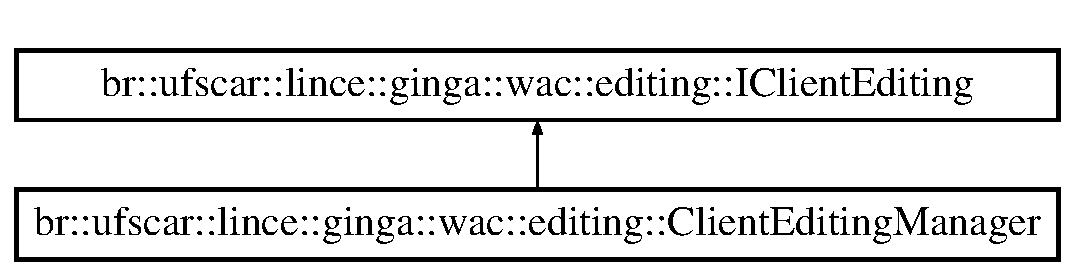
\includegraphics[height=2cm]{classbr_1_1ufscar_1_1lince_1_1ginga_1_1wac_1_1editing_1_1IClientEditing}
\end{center}
\end{figure}
\subsection*{Public Member Functions}
\begin{DoxyCompactItemize}
\item 
virtual \hyperlink{classbr_1_1ufscar_1_1lince_1_1ginga_1_1wac_1_1editing_1_1IClientEditing_a21e82d63b608e607a5618e6527cdfe23}{$\sim$IClientEditing} ()
\begin{DoxyCompactList}\small\item\em Destrói a instância de \hyperlink{classbr_1_1ufscar_1_1lince_1_1ginga_1_1wac_1_1editing_1_1IClientEditing}{IClientEditing}. \item\end{DoxyCompactList}\item 
virtual bool \hyperlink{classbr_1_1ufscar_1_1lince_1_1ginga_1_1wac_1_1editing_1_1IClientEditing_a159d8e1b676431ee5439ad932f07a6bd}{addRegion} (string regionId, LayoutRegion $\ast$layoutRegion)=0
\begin{DoxyCompactList}\small\item\em Adiciona uma Região na Versão Cliente do Documento NCL em execução. \item\end{DoxyCompactList}\item 
virtual bool \hyperlink{classbr_1_1ufscar_1_1lince_1_1ginga_1_1wac_1_1editing_1_1IClientEditing_afaa30256c70e59a36820317d203869fc}{addRegion} (string regionId, string xml)=0
\begin{DoxyCompactList}\small\item\em Adiciona uma Região na Versão Cliente do Documento NCL em execução. \item\end{DoxyCompactList}\item 
virtual bool \hyperlink{classbr_1_1ufscar_1_1lince_1_1ginga_1_1wac_1_1editing_1_1IClientEditing_abc156e111b7741a7f55c28b835614178}{addRule} (Rule $\ast$rule)=0
\begin{DoxyCompactList}\small\item\em Adiciona uma Regra na Versão Cliente do Documento NCL em execução. \item\end{DoxyCompactList}\item 
virtual bool \hyperlink{classbr_1_1ufscar_1_1lince_1_1ginga_1_1wac_1_1editing_1_1IClientEditing_a9268c1aa4301692ad9ed3c17e97d5f45}{addRule} (string xml)=0
\begin{DoxyCompactList}\small\item\em Adiciona uma Regra na Versão Cliente do Documento NCL em execução. \item\end{DoxyCompactList}\item 
virtual bool \hyperlink{classbr_1_1ufscar_1_1lince_1_1ginga_1_1wac_1_1editing_1_1IClientEditing_a1b9bb86e478437909dd6f5a77f2ff4b4}{removeRule} (string ruleId)=0
\begin{DoxyCompactList}\small\item\em Remove uma regra da Versão Cliente do Documento NCL em execução. \item\end{DoxyCompactList}\item 
virtual bool \hyperlink{classbr_1_1ufscar_1_1lince_1_1ginga_1_1wac_1_1editing_1_1IClientEditing_a8de701b01f8095605897a83002ea9fb0}{addTransition} (Transition $\ast$transition)=0
\begin{DoxyCompactList}\small\item\em Adiciona uma transição na Versão Cliente do Documento NCL em execução. \item\end{DoxyCompactList}\item 
virtual bool \hyperlink{classbr_1_1ufscar_1_1lince_1_1ginga_1_1wac_1_1editing_1_1IClientEditing_ab485ec1908e00b24e451f138446885af}{addTransition} (string xml)=0
\begin{DoxyCompactList}\small\item\em Adiciona uma transição na Versão Cliente do Documento NCL em execução. \item\end{DoxyCompactList}\item 
virtual bool \hyperlink{classbr_1_1ufscar_1_1lince_1_1ginga_1_1wac_1_1editing_1_1IClientEditing_a4f88db31bb7d754489e7cc965d9035c2}{removeTransition} (string transitionId)=0
\begin{DoxyCompactList}\small\item\em Remove uma transição da Versão Cliente do Documento NCL em execução. \item\end{DoxyCompactList}\item 
virtual bool \hyperlink{classbr_1_1ufscar_1_1lince_1_1ginga_1_1wac_1_1editing_1_1IClientEditing_ac3ce7f9f55bc61cb7166b741a73e77d9}{addConnector} (Connector $\ast$connector)=0
\begin{DoxyCompactList}\small\item\em Adiciona um Conector na Versão Cliente do Documento NCL em execução. \item\end{DoxyCompactList}\item 
virtual bool \hyperlink{classbr_1_1ufscar_1_1lince_1_1ginga_1_1wac_1_1editing_1_1IClientEditing_a531eb37bc22963dcb2feeed0e07591bd}{addConnector} (string xml)=0
\begin{DoxyCompactList}\small\item\em Adiciona um Conector na Versão Cliente do Documento NCL em execução. \item\end{DoxyCompactList}\item 
virtual bool \hyperlink{classbr_1_1ufscar_1_1lince_1_1ginga_1_1wac_1_1editing_1_1IClientEditing_a415ff450552523a495db85c15004c6f9}{removeConnector} (string connectorId)=0
\begin{DoxyCompactList}\small\item\em Remove um conector da Versão Cliente do Documento NCL em execução. \item\end{DoxyCompactList}\item 
virtual bool \hyperlink{classbr_1_1ufscar_1_1lince_1_1ginga_1_1wac_1_1editing_1_1IClientEditing_a8fb8afeaa96087d789b6b0efd9571853}{addDescriptor} (GenericDescriptor $\ast$descriptor)=0
\begin{DoxyCompactList}\small\item\em Adiciona um Descritor na Versão Cliente do Documento NCL em execução. \item\end{DoxyCompactList}\item 
virtual bool \hyperlink{classbr_1_1ufscar_1_1lince_1_1ginga_1_1wac_1_1editing_1_1IClientEditing_af7aa3b95abda814fbf7cadbd277dc2c1}{addDescriptor} (string xml)=0
\begin{DoxyCompactList}\small\item\em Adiciona um Descritor na Versão Cliente do Documento NCL em execução. \item\end{DoxyCompactList}\item 
virtual bool \hyperlink{classbr_1_1ufscar_1_1lince_1_1ginga_1_1wac_1_1editing_1_1IClientEditing_ad3ae20153844de461ded8a643443dc08}{removeDescriptor} (string descriptorId)=0
\begin{DoxyCompactList}\small\item\em Remove um descritor da Versão Cliente do Documento NCL em execução. \item\end{DoxyCompactList}\item 
virtual bool \hyperlink{classbr_1_1ufscar_1_1lince_1_1ginga_1_1wac_1_1editing_1_1IClientEditing_ad8662a9f157872a4cbe7ed0da9baf3fb}{addNode} (string compositeId, Node $\ast$node)=0
\begin{DoxyCompactList}\small\item\em Adiciona um Nó à Versão Cliente do Documento NCL em execução. \item\end{DoxyCompactList}\item 
virtual bool \hyperlink{classbr_1_1ufscar_1_1lince_1_1ginga_1_1wac_1_1editing_1_1IClientEditing_ad101947701dbbef3d365d92ae385ec46}{addNode} (string compositeId, string xml)=0
\begin{DoxyCompactList}\small\item\em Adiciona um Nó à Versão Cliente do Documento NCL em execução. \item\end{DoxyCompactList}\item 
virtual bool \hyperlink{classbr_1_1ufscar_1_1lince_1_1ginga_1_1wac_1_1editing_1_1IClientEditing_a7a733528927ed22d232ae58e0539b1eb}{addInterface} (string nodeId, InterfacePoint $\ast$interface)=0
\begin{DoxyCompactList}\small\item\em Adiciona uma Interface à Versão Cliente do Documento NCL em execução. \item\end{DoxyCompactList}\item 
virtual bool \hyperlink{classbr_1_1ufscar_1_1lince_1_1ginga_1_1wac_1_1editing_1_1IClientEditing_af60b6d775c412012b85a219311bbc4d8}{addInterface} (string nodeId, string xml)=0
\begin{DoxyCompactList}\small\item\em Adiciona uma Interface à Versão Cliente do Documento NCL em execução. \item\end{DoxyCompactList}\item 
virtual bool \hyperlink{classbr_1_1ufscar_1_1lince_1_1ginga_1_1wac_1_1editing_1_1IClientEditing_abe89650753eccb62bf1772cc0e87d6b7}{removeInterface} (string nodeId, string interfaceId)=0
\begin{DoxyCompactList}\small\item\em Remove uma interface da Versão Cliente do Documento NCL em execução. \item\end{DoxyCompactList}\item 
virtual bool \hyperlink{classbr_1_1ufscar_1_1lince_1_1ginga_1_1wac_1_1editing_1_1IClientEditing_a74829dbd18d200ef2522a0e228e20a10}{addLink} (string compositeId, Link $\ast$link)=0
\begin{DoxyCompactList}\small\item\em Adiciona um elo à Versão Cliente do Documento NCL em execução. \item\end{DoxyCompactList}\item 
virtual bool \hyperlink{classbr_1_1ufscar_1_1lince_1_1ginga_1_1wac_1_1editing_1_1IClientEditing_aa9d2c5d6522cc5428abc2a3231299b74}{addLink} (string compositeId, string xml)=0
\begin{DoxyCompactList}\small\item\em Adiciona um elo à Versão Cliente do Documento NCL em execução. \item\end{DoxyCompactList}\item 
virtual bool \hyperlink{classbr_1_1ufscar_1_1lince_1_1ginga_1_1wac_1_1editing_1_1IClientEditing_a99c3ab683d01ec8fecae2b01f7069bc4}{removeLink} (string compositeId, string linkId)=0
\begin{DoxyCompactList}\small\item\em Remove um elo da Versão Cliente do Documento NCL em execução. \item\end{DoxyCompactList}\item 
virtual NclDocument $\ast$ \hyperlink{classbr_1_1ufscar_1_1lince_1_1ginga_1_1wac_1_1editing_1_1IClientEditing_a72ba6d8611de7d1b8569a5b5d68e4fb9}{getCurrentDocument} ()=0
\begin{DoxyCompactList}\small\item\em Retorno a instância que representa o documento NCl que esta sendo apresentado. \item\end{DoxyCompactList}\item 
virtual bool \hyperlink{classbr_1_1ufscar_1_1lince_1_1ginga_1_1wac_1_1editing_1_1IClientEditing_a8b8cd2e9f79545630e04334d6366e28e}{undoLastEditing} (int n)=0
\begin{DoxyCompactList}\small\item\em Permite desfazer as ultimas edições realizadas por aplicações do cliente. \item\end{DoxyCompactList}\end{DoxyCompactItemize}


\subsection{Detailed Description}
Interface utilizada pelas aplicações do cliente para utilizar os serviçõs do módulo ClientEditig. 

\subsection{Constructor \& Destructor Documentation}
\hypertarget{classbr_1_1ufscar_1_1lince_1_1ginga_1_1wac_1_1editing_1_1IClientEditing_a21e82d63b608e607a5618e6527cdfe23}{
\index{br::ufscar::lince::ginga::wac::editing::IClientEditing@{br::ufscar::lince::ginga::wac::editing::IClientEditing}!$\sim$IClientEditing@{$\sim$IClientEditing}}
\index{$\sim$IClientEditing@{$\sim$IClientEditing}!br::ufscar::lince::ginga::wac::editing::IClientEditing@{br::ufscar::lince::ginga::wac::editing::IClientEditing}}
\subsubsection[{$\sim$IClientEditing}]{\setlength{\rightskip}{0pt plus 5cm}virtual br::ufscar::lince::ginga::wac::editing::IClientEditing::$\sim$IClientEditing ()\hspace{0.3cm}{\ttfamily  \mbox{[}inline, virtual\mbox{]}}}}
\label{classbr_1_1ufscar_1_1lince_1_1ginga_1_1wac_1_1editing_1_1IClientEditing_a21e82d63b608e607a5618e6527cdfe23}


Destrói a instância de \hyperlink{classbr_1_1ufscar_1_1lince_1_1ginga_1_1wac_1_1editing_1_1IClientEditing}{IClientEditing}. 



\subsection{Member Function Documentation}
\hypertarget{classbr_1_1ufscar_1_1lince_1_1ginga_1_1wac_1_1editing_1_1IClientEditing_a531eb37bc22963dcb2feeed0e07591bd}{
\index{br::ufscar::lince::ginga::wac::editing::IClientEditing@{br::ufscar::lince::ginga::wac::editing::IClientEditing}!addConnector@{addConnector}}
\index{addConnector@{addConnector}!br::ufscar::lince::ginga::wac::editing::IClientEditing@{br::ufscar::lince::ginga::wac::editing::IClientEditing}}
\subsubsection[{addConnector}]{\setlength{\rightskip}{0pt plus 5cm}virtual bool br::ufscar::lince::ginga::wac::editing::IClientEditing::addConnector (string {\em xml})\hspace{0.3cm}{\ttfamily  \mbox{[}pure virtual\mbox{]}}}}
\label{classbr_1_1ufscar_1_1lince_1_1ginga_1_1wac_1_1editing_1_1IClientEditing_a531eb37bc22963dcb2feeed0e07591bd}


Adiciona um Conector na Versão Cliente do Documento NCL em execução. 


\begin{DoxyParams}{Parameters}
\item[{\em xml}]Código xml do conector que será adiconado. \end{DoxyParams}
\begin{DoxyReturn}{Returns}
True se o conector foi adicionado; False caso contrário. 
\end{DoxyReturn}


Implemented in \hyperlink{classbr_1_1ufscar_1_1lince_1_1ginga_1_1wac_1_1editing_1_1ClientEditingManager_a62f5c2e221cba63f7a47c3a8ce1d154f}{br::ufscar::lince::ginga::wac::editing::ClientEditingManager}.

\hypertarget{classbr_1_1ufscar_1_1lince_1_1ginga_1_1wac_1_1editing_1_1IClientEditing_ac3ce7f9f55bc61cb7166b741a73e77d9}{
\index{br::ufscar::lince::ginga::wac::editing::IClientEditing@{br::ufscar::lince::ginga::wac::editing::IClientEditing}!addConnector@{addConnector}}
\index{addConnector@{addConnector}!br::ufscar::lince::ginga::wac::editing::IClientEditing@{br::ufscar::lince::ginga::wac::editing::IClientEditing}}
\subsubsection[{addConnector}]{\setlength{\rightskip}{0pt plus 5cm}virtual bool br::ufscar::lince::ginga::wac::editing::IClientEditing::addConnector (Connector $\ast$ {\em connector})\hspace{0.3cm}{\ttfamily  \mbox{[}pure virtual\mbox{]}}}}
\label{classbr_1_1ufscar_1_1lince_1_1ginga_1_1wac_1_1editing_1_1IClientEditing_ac3ce7f9f55bc61cb7166b741a73e77d9}


Adiciona um Conector na Versão Cliente do Documento NCL em execução. 


\begin{DoxyParams}{Parameters}
\item[{\em connector}]Instância que representa o conector que será adiconado. \end{DoxyParams}
\begin{DoxyReturn}{Returns}
True se o conector foi adicionado; False caso contrário. 
\end{DoxyReturn}


Implemented in \hyperlink{classbr_1_1ufscar_1_1lince_1_1ginga_1_1wac_1_1editing_1_1ClientEditingManager_afbc2f133a39eff4008bba3817f8c76a1}{br::ufscar::lince::ginga::wac::editing::ClientEditingManager}.

\hypertarget{classbr_1_1ufscar_1_1lince_1_1ginga_1_1wac_1_1editing_1_1IClientEditing_af7aa3b95abda814fbf7cadbd277dc2c1}{
\index{br::ufscar::lince::ginga::wac::editing::IClientEditing@{br::ufscar::lince::ginga::wac::editing::IClientEditing}!addDescriptor@{addDescriptor}}
\index{addDescriptor@{addDescriptor}!br::ufscar::lince::ginga::wac::editing::IClientEditing@{br::ufscar::lince::ginga::wac::editing::IClientEditing}}
\subsubsection[{addDescriptor}]{\setlength{\rightskip}{0pt plus 5cm}virtual bool br::ufscar::lince::ginga::wac::editing::IClientEditing::addDescriptor (string {\em xml})\hspace{0.3cm}{\ttfamily  \mbox{[}pure virtual\mbox{]}}}}
\label{classbr_1_1ufscar_1_1lince_1_1ginga_1_1wac_1_1editing_1_1IClientEditing_af7aa3b95abda814fbf7cadbd277dc2c1}


Adiciona um Descritor na Versão Cliente do Documento NCL em execução. 


\begin{DoxyParams}{Parameters}
\item[{\em xml}]Código xml do Descritor que será adiconado. \end{DoxyParams}
\begin{DoxyReturn}{Returns}
True se o Descritor foi adicionado; False caso contrário. 
\end{DoxyReturn}


Implemented in \hyperlink{classbr_1_1ufscar_1_1lince_1_1ginga_1_1wac_1_1editing_1_1ClientEditingManager_ab6fd5b9535b8d6e377aab7b7af4c2902}{br::ufscar::lince::ginga::wac::editing::ClientEditingManager}.

\hypertarget{classbr_1_1ufscar_1_1lince_1_1ginga_1_1wac_1_1editing_1_1IClientEditing_a8fb8afeaa96087d789b6b0efd9571853}{
\index{br::ufscar::lince::ginga::wac::editing::IClientEditing@{br::ufscar::lince::ginga::wac::editing::IClientEditing}!addDescriptor@{addDescriptor}}
\index{addDescriptor@{addDescriptor}!br::ufscar::lince::ginga::wac::editing::IClientEditing@{br::ufscar::lince::ginga::wac::editing::IClientEditing}}
\subsubsection[{addDescriptor}]{\setlength{\rightskip}{0pt plus 5cm}virtual bool br::ufscar::lince::ginga::wac::editing::IClientEditing::addDescriptor (GenericDescriptor $\ast$ {\em descriptor})\hspace{0.3cm}{\ttfamily  \mbox{[}pure virtual\mbox{]}}}}
\label{classbr_1_1ufscar_1_1lince_1_1ginga_1_1wac_1_1editing_1_1IClientEditing_a8fb8afeaa96087d789b6b0efd9571853}


Adiciona um Descritor na Versão Cliente do Documento NCL em execução. 


\begin{DoxyParams}{Parameters}
\item[{\em descriptor}]Instância que representa o Descritor que será adiconado. \end{DoxyParams}
\begin{DoxyReturn}{Returns}
True se o Descritor foi adicionado; False caso contrário. 
\end{DoxyReturn}


Implemented in \hyperlink{classbr_1_1ufscar_1_1lince_1_1ginga_1_1wac_1_1editing_1_1ClientEditingManager_ad43d65396682df3c57e131e5531e7e4d}{br::ufscar::lince::ginga::wac::editing::ClientEditingManager}.

\hypertarget{classbr_1_1ufscar_1_1lince_1_1ginga_1_1wac_1_1editing_1_1IClientEditing_af60b6d775c412012b85a219311bbc4d8}{
\index{br::ufscar::lince::ginga::wac::editing::IClientEditing@{br::ufscar::lince::ginga::wac::editing::IClientEditing}!addInterface@{addInterface}}
\index{addInterface@{addInterface}!br::ufscar::lince::ginga::wac::editing::IClientEditing@{br::ufscar::lince::ginga::wac::editing::IClientEditing}}
\subsubsection[{addInterface}]{\setlength{\rightskip}{0pt plus 5cm}virtual bool br::ufscar::lince::ginga::wac::editing::IClientEditing::addInterface (string {\em nodeId}, \/  string {\em xml})\hspace{0.3cm}{\ttfamily  \mbox{[}pure virtual\mbox{]}}}}
\label{classbr_1_1ufscar_1_1lince_1_1ginga_1_1wac_1_1editing_1_1IClientEditing_af60b6d775c412012b85a219311bbc4d8}


Adiciona uma Interface à Versão Cliente do Documento NCL em execução. 


\begin{DoxyParams}{Parameters}
\item[{\em nodeId}]Idenitificador do nó onde esta nova interface será adicionada. \item[{\em xml}]Código xml da interface que será adiconada. \end{DoxyParams}
\begin{DoxyReturn}{Returns}
True se a interface foi adicionada; False caso contrário. 
\end{DoxyReturn}


Implemented in \hyperlink{classbr_1_1ufscar_1_1lince_1_1ginga_1_1wac_1_1editing_1_1ClientEditingManager_a1565a7f4347ad519fc405455c603fb3c}{br::ufscar::lince::ginga::wac::editing::ClientEditingManager}.

\hypertarget{classbr_1_1ufscar_1_1lince_1_1ginga_1_1wac_1_1editing_1_1IClientEditing_a7a733528927ed22d232ae58e0539b1eb}{
\index{br::ufscar::lince::ginga::wac::editing::IClientEditing@{br::ufscar::lince::ginga::wac::editing::IClientEditing}!addInterface@{addInterface}}
\index{addInterface@{addInterface}!br::ufscar::lince::ginga::wac::editing::IClientEditing@{br::ufscar::lince::ginga::wac::editing::IClientEditing}}
\subsubsection[{addInterface}]{\setlength{\rightskip}{0pt plus 5cm}virtual bool br::ufscar::lince::ginga::wac::editing::IClientEditing::addInterface (string {\em nodeId}, \/  InterfacePoint $\ast$ {\em interface})\hspace{0.3cm}{\ttfamily  \mbox{[}pure virtual\mbox{]}}}}
\label{classbr_1_1ufscar_1_1lince_1_1ginga_1_1wac_1_1editing_1_1IClientEditing_a7a733528927ed22d232ae58e0539b1eb}


Adiciona uma Interface à Versão Cliente do Documento NCL em execução. 


\begin{DoxyParams}{Parameters}
\item[{\em nodeId}]Idenitificador do nó onde esta nova interface será adicionada. \item[{\em interface}]Instância que representa a interface que será adiconada. \end{DoxyParams}
\begin{DoxyReturn}{Returns}
True se a interface foi adicionada; False caso contrário. 
\end{DoxyReturn}


Implemented in \hyperlink{classbr_1_1ufscar_1_1lince_1_1ginga_1_1wac_1_1editing_1_1ClientEditingManager_a7e6eaecc65141d2660bdb1b1c33c421f}{br::ufscar::lince::ginga::wac::editing::ClientEditingManager}.

\hypertarget{classbr_1_1ufscar_1_1lince_1_1ginga_1_1wac_1_1editing_1_1IClientEditing_aa9d2c5d6522cc5428abc2a3231299b74}{
\index{br::ufscar::lince::ginga::wac::editing::IClientEditing@{br::ufscar::lince::ginga::wac::editing::IClientEditing}!addLink@{addLink}}
\index{addLink@{addLink}!br::ufscar::lince::ginga::wac::editing::IClientEditing@{br::ufscar::lince::ginga::wac::editing::IClientEditing}}
\subsubsection[{addLink}]{\setlength{\rightskip}{0pt plus 5cm}virtual bool br::ufscar::lince::ginga::wac::editing::IClientEditing::addLink (string {\em compositeId}, \/  string {\em xml})\hspace{0.3cm}{\ttfamily  \mbox{[}pure virtual\mbox{]}}}}
\label{classbr_1_1ufscar_1_1lince_1_1ginga_1_1wac_1_1editing_1_1IClientEditing_aa9d2c5d6522cc5428abc2a3231299b74}


Adiciona um elo à Versão Cliente do Documento NCL em execução. 


\begin{DoxyParams}{Parameters}
\item[{\em compositeId}]Idenitificador do nó de contexto onde este novo elo será adicionado. \item[{\em xml}]Código xml do elo que será adiconado. \end{DoxyParams}
\begin{DoxyReturn}{Returns}
True se o elo foi adicionado; False caso contrário. 
\end{DoxyReturn}


Implemented in \hyperlink{classbr_1_1ufscar_1_1lince_1_1ginga_1_1wac_1_1editing_1_1ClientEditingManager_a88c07d75d150d08724ec077fa54f2aeb}{br::ufscar::lince::ginga::wac::editing::ClientEditingManager}.

\hypertarget{classbr_1_1ufscar_1_1lince_1_1ginga_1_1wac_1_1editing_1_1IClientEditing_a74829dbd18d200ef2522a0e228e20a10}{
\index{br::ufscar::lince::ginga::wac::editing::IClientEditing@{br::ufscar::lince::ginga::wac::editing::IClientEditing}!addLink@{addLink}}
\index{addLink@{addLink}!br::ufscar::lince::ginga::wac::editing::IClientEditing@{br::ufscar::lince::ginga::wac::editing::IClientEditing}}
\subsubsection[{addLink}]{\setlength{\rightskip}{0pt plus 5cm}virtual bool br::ufscar::lince::ginga::wac::editing::IClientEditing::addLink (string {\em compositeId}, \/  Link $\ast$ {\em link})\hspace{0.3cm}{\ttfamily  \mbox{[}pure virtual\mbox{]}}}}
\label{classbr_1_1ufscar_1_1lince_1_1ginga_1_1wac_1_1editing_1_1IClientEditing_a74829dbd18d200ef2522a0e228e20a10}


Adiciona um elo à Versão Cliente do Documento NCL em execução. 


\begin{DoxyParams}{Parameters}
\item[{\em compositeId}]Idenitificador do nó de contexto onde este novo elo será adicionado. \item[{\em link}]Instancia que representa o elo que será adiconado. \end{DoxyParams}
\begin{DoxyReturn}{Returns}
True se o elo foi adicionado; False caso contrário. 
\end{DoxyReturn}


Implemented in \hyperlink{classbr_1_1ufscar_1_1lince_1_1ginga_1_1wac_1_1editing_1_1ClientEditingManager_a53cb5ddc1e425c7f03c7aacff140223c}{br::ufscar::lince::ginga::wac::editing::ClientEditingManager}.

\hypertarget{classbr_1_1ufscar_1_1lince_1_1ginga_1_1wac_1_1editing_1_1IClientEditing_ad101947701dbbef3d365d92ae385ec46}{
\index{br::ufscar::lince::ginga::wac::editing::IClientEditing@{br::ufscar::lince::ginga::wac::editing::IClientEditing}!addNode@{addNode}}
\index{addNode@{addNode}!br::ufscar::lince::ginga::wac::editing::IClientEditing@{br::ufscar::lince::ginga::wac::editing::IClientEditing}}
\subsubsection[{addNode}]{\setlength{\rightskip}{0pt plus 5cm}virtual bool br::ufscar::lince::ginga::wac::editing::IClientEditing::addNode (string {\em compositeId}, \/  string {\em xml})\hspace{0.3cm}{\ttfamily  \mbox{[}pure virtual\mbox{]}}}}
\label{classbr_1_1ufscar_1_1lince_1_1ginga_1_1wac_1_1editing_1_1IClientEditing_ad101947701dbbef3d365d92ae385ec46}


Adiciona um Nó à Versão Cliente do Documento NCL em execução. 


\begin{DoxyParams}{Parameters}
\item[{\em compositeId}]Idenitificador do nó onde este novo nó será adicionado. \item[{\em xml}]Código xml do nó que será adiconado. \end{DoxyParams}
\begin{DoxyReturn}{Returns}
True se o nó foi adicionado; False caso contrário. 
\end{DoxyReturn}


Implemented in \hyperlink{classbr_1_1ufscar_1_1lince_1_1ginga_1_1wac_1_1editing_1_1ClientEditingManager_aa7ddb3cd14fd26fe7e4edf8b3024fdb7}{br::ufscar::lince::ginga::wac::editing::ClientEditingManager}.

\hypertarget{classbr_1_1ufscar_1_1lince_1_1ginga_1_1wac_1_1editing_1_1IClientEditing_ad8662a9f157872a4cbe7ed0da9baf3fb}{
\index{br::ufscar::lince::ginga::wac::editing::IClientEditing@{br::ufscar::lince::ginga::wac::editing::IClientEditing}!addNode@{addNode}}
\index{addNode@{addNode}!br::ufscar::lince::ginga::wac::editing::IClientEditing@{br::ufscar::lince::ginga::wac::editing::IClientEditing}}
\subsubsection[{addNode}]{\setlength{\rightskip}{0pt plus 5cm}virtual bool br::ufscar::lince::ginga::wac::editing::IClientEditing::addNode (string {\em compositeId}, \/  Node $\ast$ {\em node})\hspace{0.3cm}{\ttfamily  \mbox{[}pure virtual\mbox{]}}}}
\label{classbr_1_1ufscar_1_1lince_1_1ginga_1_1wac_1_1editing_1_1IClientEditing_ad8662a9f157872a4cbe7ed0da9baf3fb}


Adiciona um Nó à Versão Cliente do Documento NCL em execução. 


\begin{DoxyParams}{Parameters}
\item[{\em compositeId}]Idenitificador do nó onde este novo nó será adicionado. \item[{\em node}]Instância que representa o nó que será adiconado. \end{DoxyParams}
\begin{DoxyReturn}{Returns}
True se o nó foi adicionado; False caso contrário. 
\end{DoxyReturn}


Implemented in \hyperlink{classbr_1_1ufscar_1_1lince_1_1ginga_1_1wac_1_1editing_1_1ClientEditingManager_a8e27f52402bb58a3e49d63b28652b2b9}{br::ufscar::lince::ginga::wac::editing::ClientEditingManager}.

\hypertarget{classbr_1_1ufscar_1_1lince_1_1ginga_1_1wac_1_1editing_1_1IClientEditing_afaa30256c70e59a36820317d203869fc}{
\index{br::ufscar::lince::ginga::wac::editing::IClientEditing@{br::ufscar::lince::ginga::wac::editing::IClientEditing}!addRegion@{addRegion}}
\index{addRegion@{addRegion}!br::ufscar::lince::ginga::wac::editing::IClientEditing@{br::ufscar::lince::ginga::wac::editing::IClientEditing}}
\subsubsection[{addRegion}]{\setlength{\rightskip}{0pt plus 5cm}virtual bool br::ufscar::lince::ginga::wac::editing::IClientEditing::addRegion (string {\em regionId}, \/  string {\em xml})\hspace{0.3cm}{\ttfamily  \mbox{[}pure virtual\mbox{]}}}}
\label{classbr_1_1ufscar_1_1lince_1_1ginga_1_1wac_1_1editing_1_1IClientEditing_afaa30256c70e59a36820317d203869fc}


Adiciona uma Região na Versão Cliente do Documento NCL em execução. 


\begin{DoxyParams}{Parameters}
\item[{\em regionId}]Identificador da Região onde a nova Região será adiconada. \item[{\em xml}]Código xml da Região que será adiconada. \end{DoxyParams}
\begin{DoxyReturn}{Returns}
True se a região foi adicionada; False caso contrário. 
\end{DoxyReturn}


Implemented in \hyperlink{classbr_1_1ufscar_1_1lince_1_1ginga_1_1wac_1_1editing_1_1ClientEditingManager_a4f4a856d51b586312be91b376ec0d8f3}{br::ufscar::lince::ginga::wac::editing::ClientEditingManager}.

\hypertarget{classbr_1_1ufscar_1_1lince_1_1ginga_1_1wac_1_1editing_1_1IClientEditing_a159d8e1b676431ee5439ad932f07a6bd}{
\index{br::ufscar::lince::ginga::wac::editing::IClientEditing@{br::ufscar::lince::ginga::wac::editing::IClientEditing}!addRegion@{addRegion}}
\index{addRegion@{addRegion}!br::ufscar::lince::ginga::wac::editing::IClientEditing@{br::ufscar::lince::ginga::wac::editing::IClientEditing}}
\subsubsection[{addRegion}]{\setlength{\rightskip}{0pt plus 5cm}virtual bool br::ufscar::lince::ginga::wac::editing::IClientEditing::addRegion (string {\em regionId}, \/  LayoutRegion $\ast$ {\em layoutRegion})\hspace{0.3cm}{\ttfamily  \mbox{[}pure virtual\mbox{]}}}}
\label{classbr_1_1ufscar_1_1lince_1_1ginga_1_1wac_1_1editing_1_1IClientEditing_a159d8e1b676431ee5439ad932f07a6bd}


Adiciona uma Região na Versão Cliente do Documento NCL em execução. 


\begin{DoxyParams}{Parameters}
\item[{\em regionId}]Identificador da Região onde a nova Região será adiconada. \item[{\em layoutRegion}]Instância que representa a Região que será adiconada. \end{DoxyParams}
\begin{DoxyReturn}{Returns}
True se a região foi adicionada; False caso contrário. 
\end{DoxyReturn}


Implemented in \hyperlink{classbr_1_1ufscar_1_1lince_1_1ginga_1_1wac_1_1editing_1_1ClientEditingManager_a554a556985da2aaa32fe3c705d957705}{br::ufscar::lince::ginga::wac::editing::ClientEditingManager}.

\hypertarget{classbr_1_1ufscar_1_1lince_1_1ginga_1_1wac_1_1editing_1_1IClientEditing_a9268c1aa4301692ad9ed3c17e97d5f45}{
\index{br::ufscar::lince::ginga::wac::editing::IClientEditing@{br::ufscar::lince::ginga::wac::editing::IClientEditing}!addRule@{addRule}}
\index{addRule@{addRule}!br::ufscar::lince::ginga::wac::editing::IClientEditing@{br::ufscar::lince::ginga::wac::editing::IClientEditing}}
\subsubsection[{addRule}]{\setlength{\rightskip}{0pt plus 5cm}virtual bool br::ufscar::lince::ginga::wac::editing::IClientEditing::addRule (string {\em xml})\hspace{0.3cm}{\ttfamily  \mbox{[}pure virtual\mbox{]}}}}
\label{classbr_1_1ufscar_1_1lince_1_1ginga_1_1wac_1_1editing_1_1IClientEditing_a9268c1aa4301692ad9ed3c17e97d5f45}


Adiciona uma Regra na Versão Cliente do Documento NCL em execução. 


\begin{DoxyParams}{Parameters}
\item[{\em xml}]Código xml da Regra que será adiconada. \end{DoxyParams}
\begin{DoxyReturn}{Returns}
True se a regra foi adicionada; False caso contrário. 
\end{DoxyReturn}


Implemented in \hyperlink{classbr_1_1ufscar_1_1lince_1_1ginga_1_1wac_1_1editing_1_1ClientEditingManager_abbf0ba0c717c55996fac349a88f78b6f}{br::ufscar::lince::ginga::wac::editing::ClientEditingManager}.

\hypertarget{classbr_1_1ufscar_1_1lince_1_1ginga_1_1wac_1_1editing_1_1IClientEditing_abc156e111b7741a7f55c28b835614178}{
\index{br::ufscar::lince::ginga::wac::editing::IClientEditing@{br::ufscar::lince::ginga::wac::editing::IClientEditing}!addRule@{addRule}}
\index{addRule@{addRule}!br::ufscar::lince::ginga::wac::editing::IClientEditing@{br::ufscar::lince::ginga::wac::editing::IClientEditing}}
\subsubsection[{addRule}]{\setlength{\rightskip}{0pt plus 5cm}virtual bool br::ufscar::lince::ginga::wac::editing::IClientEditing::addRule (Rule $\ast$ {\em rule})\hspace{0.3cm}{\ttfamily  \mbox{[}pure virtual\mbox{]}}}}
\label{classbr_1_1ufscar_1_1lince_1_1ginga_1_1wac_1_1editing_1_1IClientEditing_abc156e111b7741a7f55c28b835614178}


Adiciona uma Regra na Versão Cliente do Documento NCL em execução. 


\begin{DoxyParams}{Parameters}
\item[{\em rule}]Instância que representa a Regra que será adiconada. \end{DoxyParams}
\begin{DoxyReturn}{Returns}
True se a regra foi adicionada; False caso contrário. 
\end{DoxyReturn}


Implemented in \hyperlink{classbr_1_1ufscar_1_1lince_1_1ginga_1_1wac_1_1editing_1_1ClientEditingManager_a21f7109da6d0eb0b54629547513ff69e}{br::ufscar::lince::ginga::wac::editing::ClientEditingManager}.

\hypertarget{classbr_1_1ufscar_1_1lince_1_1ginga_1_1wac_1_1editing_1_1IClientEditing_ab485ec1908e00b24e451f138446885af}{
\index{br::ufscar::lince::ginga::wac::editing::IClientEditing@{br::ufscar::lince::ginga::wac::editing::IClientEditing}!addTransition@{addTransition}}
\index{addTransition@{addTransition}!br::ufscar::lince::ginga::wac::editing::IClientEditing@{br::ufscar::lince::ginga::wac::editing::IClientEditing}}
\subsubsection[{addTransition}]{\setlength{\rightskip}{0pt plus 5cm}virtual bool br::ufscar::lince::ginga::wac::editing::IClientEditing::addTransition (string {\em xml})\hspace{0.3cm}{\ttfamily  \mbox{[}pure virtual\mbox{]}}}}
\label{classbr_1_1ufscar_1_1lince_1_1ginga_1_1wac_1_1editing_1_1IClientEditing_ab485ec1908e00b24e451f138446885af}


Adiciona uma transição na Versão Cliente do Documento NCL em execução. 


\begin{DoxyParams}{Parameters}
\item[{\em xml}]Código xml da transição que será adiconada. \end{DoxyParams}
\begin{DoxyReturn}{Returns}
True se a transição foi adicionada; False caso contrário. 
\end{DoxyReturn}


Implemented in \hyperlink{classbr_1_1ufscar_1_1lince_1_1ginga_1_1wac_1_1editing_1_1ClientEditingManager_a474cdd2a429ab96cb5376264ff38fa31}{br::ufscar::lince::ginga::wac::editing::ClientEditingManager}.

\hypertarget{classbr_1_1ufscar_1_1lince_1_1ginga_1_1wac_1_1editing_1_1IClientEditing_a8de701b01f8095605897a83002ea9fb0}{
\index{br::ufscar::lince::ginga::wac::editing::IClientEditing@{br::ufscar::lince::ginga::wac::editing::IClientEditing}!addTransition@{addTransition}}
\index{addTransition@{addTransition}!br::ufscar::lince::ginga::wac::editing::IClientEditing@{br::ufscar::lince::ginga::wac::editing::IClientEditing}}
\subsubsection[{addTransition}]{\setlength{\rightskip}{0pt plus 5cm}virtual bool br::ufscar::lince::ginga::wac::editing::IClientEditing::addTransition (Transition $\ast$ {\em transition})\hspace{0.3cm}{\ttfamily  \mbox{[}pure virtual\mbox{]}}}}
\label{classbr_1_1ufscar_1_1lince_1_1ginga_1_1wac_1_1editing_1_1IClientEditing_a8de701b01f8095605897a83002ea9fb0}


Adiciona uma transição na Versão Cliente do Documento NCL em execução. 


\begin{DoxyParams}{Parameters}
\item[{\em transition}]Instância que representa a transição que será adiconada. \end{DoxyParams}
\begin{DoxyReturn}{Returns}
True se a transição foi adicionada; False caso contrário. 
\end{DoxyReturn}


Implemented in \hyperlink{classbr_1_1ufscar_1_1lince_1_1ginga_1_1wac_1_1editing_1_1ClientEditingManager_af872bea61e20e96b7ef968e24627d8c7}{br::ufscar::lince::ginga::wac::editing::ClientEditingManager}.

\hypertarget{classbr_1_1ufscar_1_1lince_1_1ginga_1_1wac_1_1editing_1_1IClientEditing_a72ba6d8611de7d1b8569a5b5d68e4fb9}{
\index{br::ufscar::lince::ginga::wac::editing::IClientEditing@{br::ufscar::lince::ginga::wac::editing::IClientEditing}!getCurrentDocument@{getCurrentDocument}}
\index{getCurrentDocument@{getCurrentDocument}!br::ufscar::lince::ginga::wac::editing::IClientEditing@{br::ufscar::lince::ginga::wac::editing::IClientEditing}}
\subsubsection[{getCurrentDocument}]{\setlength{\rightskip}{0pt plus 5cm}virtual NclDocument$\ast$ br::ufscar::lince::ginga::wac::editing::IClientEditing::getCurrentDocument ()\hspace{0.3cm}{\ttfamily  \mbox{[}pure virtual\mbox{]}}}}
\label{classbr_1_1ufscar_1_1lince_1_1ginga_1_1wac_1_1editing_1_1IClientEditing_a72ba6d8611de7d1b8569a5b5d68e4fb9}


Retorno a instância que representa o documento NCl que esta sendo apresentado. 

\begin{DoxyReturn}{Returns}
Documento NCL que está sendo apresentado. 
\end{DoxyReturn}


Implemented in \hyperlink{classbr_1_1ufscar_1_1lince_1_1ginga_1_1wac_1_1editing_1_1ClientEditingManager_a49b1b969381d54583a4c0ae61756ba7b}{br::ufscar::lince::ginga::wac::editing::ClientEditingManager}.

\hypertarget{classbr_1_1ufscar_1_1lince_1_1ginga_1_1wac_1_1editing_1_1IClientEditing_a415ff450552523a495db85c15004c6f9}{
\index{br::ufscar::lince::ginga::wac::editing::IClientEditing@{br::ufscar::lince::ginga::wac::editing::IClientEditing}!removeConnector@{removeConnector}}
\index{removeConnector@{removeConnector}!br::ufscar::lince::ginga::wac::editing::IClientEditing@{br::ufscar::lince::ginga::wac::editing::IClientEditing}}
\subsubsection[{removeConnector}]{\setlength{\rightskip}{0pt plus 5cm}virtual bool br::ufscar::lince::ginga::wac::editing::IClientEditing::removeConnector (string {\em connectorId})\hspace{0.3cm}{\ttfamily  \mbox{[}pure virtual\mbox{]}}}}
\label{classbr_1_1ufscar_1_1lince_1_1ginga_1_1wac_1_1editing_1_1IClientEditing_a415ff450552523a495db85c15004c6f9}


Remove um conector da Versão Cliente do Documento NCL em execução. 


\begin{DoxyParams}{Parameters}
\item[{\em connectorId}]Identificador do conector que será removido. \end{DoxyParams}
\begin{DoxyReturn}{Returns}
True se o conector for removido; False caso contrário. 
\end{DoxyReturn}


Implemented in \hyperlink{classbr_1_1ufscar_1_1lince_1_1ginga_1_1wac_1_1editing_1_1ClientEditingManager_a5b6ddc8a6259b07eae8f2c2f03dcdfaa}{br::ufscar::lince::ginga::wac::editing::ClientEditingManager}.

\hypertarget{classbr_1_1ufscar_1_1lince_1_1ginga_1_1wac_1_1editing_1_1IClientEditing_ad3ae20153844de461ded8a643443dc08}{
\index{br::ufscar::lince::ginga::wac::editing::IClientEditing@{br::ufscar::lince::ginga::wac::editing::IClientEditing}!removeDescriptor@{removeDescriptor}}
\index{removeDescriptor@{removeDescriptor}!br::ufscar::lince::ginga::wac::editing::IClientEditing@{br::ufscar::lince::ginga::wac::editing::IClientEditing}}
\subsubsection[{removeDescriptor}]{\setlength{\rightskip}{0pt plus 5cm}virtual bool br::ufscar::lince::ginga::wac::editing::IClientEditing::removeDescriptor (string {\em descriptorId})\hspace{0.3cm}{\ttfamily  \mbox{[}pure virtual\mbox{]}}}}
\label{classbr_1_1ufscar_1_1lince_1_1ginga_1_1wac_1_1editing_1_1IClientEditing_ad3ae20153844de461ded8a643443dc08}


Remove um descritor da Versão Cliente do Documento NCL em execução. 


\begin{DoxyParams}{Parameters}
\item[{\em descriptorId}]Identificador do descritor que será removido. \end{DoxyParams}
\begin{DoxyReturn}{Returns}
True se o descritor for removido; False caso contrário. 
\end{DoxyReturn}


Implemented in \hyperlink{classbr_1_1ufscar_1_1lince_1_1ginga_1_1wac_1_1editing_1_1ClientEditingManager_a9b25cb3580c52ddb8147ede64ec53077}{br::ufscar::lince::ginga::wac::editing::ClientEditingManager}.

\hypertarget{classbr_1_1ufscar_1_1lince_1_1ginga_1_1wac_1_1editing_1_1IClientEditing_abe89650753eccb62bf1772cc0e87d6b7}{
\index{br::ufscar::lince::ginga::wac::editing::IClientEditing@{br::ufscar::lince::ginga::wac::editing::IClientEditing}!removeInterface@{removeInterface}}
\index{removeInterface@{removeInterface}!br::ufscar::lince::ginga::wac::editing::IClientEditing@{br::ufscar::lince::ginga::wac::editing::IClientEditing}}
\subsubsection[{removeInterface}]{\setlength{\rightskip}{0pt plus 5cm}virtual bool br::ufscar::lince::ginga::wac::editing::IClientEditing::removeInterface (string {\em nodeId}, \/  string {\em interfaceId})\hspace{0.3cm}{\ttfamily  \mbox{[}pure virtual\mbox{]}}}}
\label{classbr_1_1ufscar_1_1lince_1_1ginga_1_1wac_1_1editing_1_1IClientEditing_abe89650753eccb62bf1772cc0e87d6b7}


Remove uma interface da Versão Cliente do Documento NCL em execução. 


\begin{DoxyParams}{Parameters}
\item[{\em nodeId}]Idenitificador do nó de onde esta interface será removida. \item[{\em descriptorId}]Identificador do descritor que será removido. \end{DoxyParams}
\begin{DoxyReturn}{Returns}
True se o descritor for removido; False caso contrário. 
\end{DoxyReturn}


Implemented in \hyperlink{classbr_1_1ufscar_1_1lince_1_1ginga_1_1wac_1_1editing_1_1ClientEditingManager_a23d60db841bf10edd6266de52613b9b2}{br::ufscar::lince::ginga::wac::editing::ClientEditingManager}.

\hypertarget{classbr_1_1ufscar_1_1lince_1_1ginga_1_1wac_1_1editing_1_1IClientEditing_a99c3ab683d01ec8fecae2b01f7069bc4}{
\index{br::ufscar::lince::ginga::wac::editing::IClientEditing@{br::ufscar::lince::ginga::wac::editing::IClientEditing}!removeLink@{removeLink}}
\index{removeLink@{removeLink}!br::ufscar::lince::ginga::wac::editing::IClientEditing@{br::ufscar::lince::ginga::wac::editing::IClientEditing}}
\subsubsection[{removeLink}]{\setlength{\rightskip}{0pt plus 5cm}virtual bool br::ufscar::lince::ginga::wac::editing::IClientEditing::removeLink (string {\em compositeId}, \/  string {\em linkId})\hspace{0.3cm}{\ttfamily  \mbox{[}pure virtual\mbox{]}}}}
\label{classbr_1_1ufscar_1_1lince_1_1ginga_1_1wac_1_1editing_1_1IClientEditing_a99c3ab683d01ec8fecae2b01f7069bc4}


Remove um elo da Versão Cliente do Documento NCL em execução. 


\begin{DoxyParams}{Parameters}
\item[{\em nodeId}]Idenitificador do nó de onde este elo será removido. \item[{\em descriptorId}]Identificador do elo que será removido. \end{DoxyParams}
\begin{DoxyReturn}{Returns}
True se o elo for removido; False caso contrário. 
\end{DoxyReturn}


Implemented in \hyperlink{classbr_1_1ufscar_1_1lince_1_1ginga_1_1wac_1_1editing_1_1ClientEditingManager_a11e5f1029545aa4c0435094cc59477cb}{br::ufscar::lince::ginga::wac::editing::ClientEditingManager}.

\hypertarget{classbr_1_1ufscar_1_1lince_1_1ginga_1_1wac_1_1editing_1_1IClientEditing_a1b9bb86e478437909dd6f5a77f2ff4b4}{
\index{br::ufscar::lince::ginga::wac::editing::IClientEditing@{br::ufscar::lince::ginga::wac::editing::IClientEditing}!removeRule@{removeRule}}
\index{removeRule@{removeRule}!br::ufscar::lince::ginga::wac::editing::IClientEditing@{br::ufscar::lince::ginga::wac::editing::IClientEditing}}
\subsubsection[{removeRule}]{\setlength{\rightskip}{0pt plus 5cm}virtual bool br::ufscar::lince::ginga::wac::editing::IClientEditing::removeRule (string {\em ruleId})\hspace{0.3cm}{\ttfamily  \mbox{[}pure virtual\mbox{]}}}}
\label{classbr_1_1ufscar_1_1lince_1_1ginga_1_1wac_1_1editing_1_1IClientEditing_a1b9bb86e478437909dd6f5a77f2ff4b4}


Remove uma regra da Versão Cliente do Documento NCL em execução. 


\begin{DoxyParams}{Parameters}
\item[{\em ruleId}]Identificador da Regra que será removida. \end{DoxyParams}
\begin{DoxyReturn}{Returns}
True se a regra for removida; False caso contrário. 
\end{DoxyReturn}


Implemented in \hyperlink{classbr_1_1ufscar_1_1lince_1_1ginga_1_1wac_1_1editing_1_1ClientEditingManager_a5b363245776a5a71bd3c7628dcf91f7e}{br::ufscar::lince::ginga::wac::editing::ClientEditingManager}.

\hypertarget{classbr_1_1ufscar_1_1lince_1_1ginga_1_1wac_1_1editing_1_1IClientEditing_a4f88db31bb7d754489e7cc965d9035c2}{
\index{br::ufscar::lince::ginga::wac::editing::IClientEditing@{br::ufscar::lince::ginga::wac::editing::IClientEditing}!removeTransition@{removeTransition}}
\index{removeTransition@{removeTransition}!br::ufscar::lince::ginga::wac::editing::IClientEditing@{br::ufscar::lince::ginga::wac::editing::IClientEditing}}
\subsubsection[{removeTransition}]{\setlength{\rightskip}{0pt plus 5cm}virtual bool br::ufscar::lince::ginga::wac::editing::IClientEditing::removeTransition (string {\em transitionId})\hspace{0.3cm}{\ttfamily  \mbox{[}pure virtual\mbox{]}}}}
\label{classbr_1_1ufscar_1_1lince_1_1ginga_1_1wac_1_1editing_1_1IClientEditing_a4f88db31bb7d754489e7cc965d9035c2}


Remove uma transição da Versão Cliente do Documento NCL em execução. 


\begin{DoxyParams}{Parameters}
\item[{\em transitionId}]Identificador da transição que será removida. \end{DoxyParams}
\begin{DoxyReturn}{Returns}
True se a transição for removida; False caso contrário. 
\end{DoxyReturn}


Implemented in \hyperlink{classbr_1_1ufscar_1_1lince_1_1ginga_1_1wac_1_1editing_1_1ClientEditingManager_a6aebcca439720cc2c9b69d6b7b5c45c7}{br::ufscar::lince::ginga::wac::editing::ClientEditingManager}.

\hypertarget{classbr_1_1ufscar_1_1lince_1_1ginga_1_1wac_1_1editing_1_1IClientEditing_a8b8cd2e9f79545630e04334d6366e28e}{
\index{br::ufscar::lince::ginga::wac::editing::IClientEditing@{br::ufscar::lince::ginga::wac::editing::IClientEditing}!undoLastEditing@{undoLastEditing}}
\index{undoLastEditing@{undoLastEditing}!br::ufscar::lince::ginga::wac::editing::IClientEditing@{br::ufscar::lince::ginga::wac::editing::IClientEditing}}
\subsubsection[{undoLastEditing}]{\setlength{\rightskip}{0pt plus 5cm}virtual bool br::ufscar::lince::ginga::wac::editing::IClientEditing::undoLastEditing (int {\em n})\hspace{0.3cm}{\ttfamily  \mbox{[}pure virtual\mbox{]}}}}
\label{classbr_1_1ufscar_1_1lince_1_1ginga_1_1wac_1_1editing_1_1IClientEditing_a8b8cd2e9f79545630e04334d6366e28e}


Permite desfazer as ultimas edições realizadas por aplicações do cliente. 


\begin{DoxyParams}{Parameters}
\item[{\em n}]Número de edições que serão desfeitas. Se omitido será desfeita uma edição. \end{DoxyParams}
\begin{DoxyReturn}{Returns}
True se as alterações foram desfeitas com sucesso; False Caso contrário. 
\end{DoxyReturn}


Implemented in \hyperlink{classbr_1_1ufscar_1_1lince_1_1ginga_1_1wac_1_1editing_1_1ClientEditingManager_a7094577521bafedebcd7edafe753774f}{br::ufscar::lince::ginga::wac::editing::ClientEditingManager}.



The documentation for this class was generated from the following file:\begin{DoxyCompactItemize}
\item 
include/\hyperlink{IClientEditing_8h}{IClientEditing.h}\end{DoxyCompactItemize}

\hypertarget{classbr_1_1ufscar_1_1lince_1_1ginga_1_1wac_1_1editing_1_1IFormatterAdapter}{
\section{br::ufscar::lince::ginga::wac::editing::IFormatterAdapter Class Reference}
\label{classbr_1_1ufscar_1_1lince_1_1ginga_1_1wac_1_1editing_1_1IFormatterAdapter}\index{br::ufscar::lince::ginga::wac::editing::IFormatterAdapter@{br::ufscar::lince::ginga::wac::editing::IFormatterAdapter}}
}


Interface que permite que as classes do módulo Wac-\/Editing enviem mensagem a classe Formatter do módulo Formatter.  




{\ttfamily \#include $<$IFormatterAdapter.h$>$}

\subsection*{Public Member Functions}
\begin{DoxyCompactItemize}
\item 
virtual \hyperlink{classbr_1_1ufscar_1_1lince_1_1ginga_1_1wac_1_1editing_1_1IFormatterAdapter_aa2e061e9d4bd5af9ee7abc5354d4f1a7}{$\sim$IFormatterAdapter} ()
\begin{DoxyCompactList}\small\item\em Destrói \hyperlink{classbr_1_1ufscar_1_1lince_1_1ginga_1_1wac_1_1editing_1_1IFormatterAdapter}{IFormatterAdapter}. \item\end{DoxyCompactList}\item 
virtual LayoutRegion $\ast$ \hyperlink{classbr_1_1ufscar_1_1lince_1_1ginga_1_1wac_1_1editing_1_1IFormatterAdapter_a379cbb803df82804f69730a554026081}{addRegion} (string compositeDocumentId, string regionId, string xmlRegion, int=\hyperlink{classbr_1_1ufscar_1_1lince_1_1ginga_1_1wac_1_1editing_1_1IFormatterAdapter_a60586f9a11e5cefcfecef9386c28d4bd}{BROADCASTER\_\-EDITING})=0
\item 
virtual LayoutRegion $\ast$ \hyperlink{classbr_1_1ufscar_1_1lince_1_1ginga_1_1wac_1_1editing_1_1IFormatterAdapter_a7451f3f638fd722aabaacf2674620e13}{removeRegion} (string compositeDocumentId, string regionId, int=\hyperlink{classbr_1_1ufscar_1_1lince_1_1ginga_1_1wac_1_1editing_1_1IFormatterAdapter_a60586f9a11e5cefcfecef9386c28d4bd}{BROADCASTER\_\-EDITING})=0
\item 
virtual RegionBase $\ast$ \hyperlink{classbr_1_1ufscar_1_1lince_1_1ginga_1_1wac_1_1editing_1_1IFormatterAdapter_abef17b93da126eef818bafdbbde2f0ab}{addRegionBase} (string compositeDocumentId, string xmlRegionBase, int=\hyperlink{classbr_1_1ufscar_1_1lince_1_1ginga_1_1wac_1_1editing_1_1IFormatterAdapter_a60586f9a11e5cefcfecef9386c28d4bd}{BROADCASTER\_\-EDITING})=0
\item 
virtual RegionBase $\ast$ \hyperlink{classbr_1_1ufscar_1_1lince_1_1ginga_1_1wac_1_1editing_1_1IFormatterAdapter_a1994d2a14c28cd577919f3988b224f00}{removeRegionBase} (string compositeDocumentId, string regionBaseId, int=\hyperlink{classbr_1_1ufscar_1_1lince_1_1ginga_1_1wac_1_1editing_1_1IFormatterAdapter_a60586f9a11e5cefcfecef9386c28d4bd}{BROADCASTER\_\-EDITING})=0
\item 
virtual Rule $\ast$ \hyperlink{classbr_1_1ufscar_1_1lince_1_1ginga_1_1wac_1_1editing_1_1IFormatterAdapter_aebdea3839c00805a61f5f4229e6d5f6f}{addRule} (string compositeDocumentId, string xmlRule, int=\hyperlink{classbr_1_1ufscar_1_1lince_1_1ginga_1_1wac_1_1editing_1_1IFormatterAdapter_a60586f9a11e5cefcfecef9386c28d4bd}{BROADCASTER\_\-EDITING})=0
\item 
virtual Rule $\ast$ \hyperlink{classbr_1_1ufscar_1_1lince_1_1ginga_1_1wac_1_1editing_1_1IFormatterAdapter_ab50348d88204b6e715d1fd14ad485661}{removeRule} (string compositeDocumentId, string ruleId, int=\hyperlink{classbr_1_1ufscar_1_1lince_1_1ginga_1_1wac_1_1editing_1_1IFormatterAdapter_a60586f9a11e5cefcfecef9386c28d4bd}{BROADCASTER\_\-EDITING})=0
\item 
virtual RuleBase $\ast$ \hyperlink{classbr_1_1ufscar_1_1lince_1_1ginga_1_1wac_1_1editing_1_1IFormatterAdapter_a0d65630a7f103c38c04e06c8a584ecba}{addRuleBase} (string compositeDocumentId, string xmlRuleBase, int=\hyperlink{classbr_1_1ufscar_1_1lince_1_1ginga_1_1wac_1_1editing_1_1IFormatterAdapter_a60586f9a11e5cefcfecef9386c28d4bd}{BROADCASTER\_\-EDITING})=0
\item 
virtual RuleBase $\ast$ \hyperlink{classbr_1_1ufscar_1_1lince_1_1ginga_1_1wac_1_1editing_1_1IFormatterAdapter_a9b854fb32b46e6e16557cf2fc24e2f09}{removeRuleBase} (string compositeDocumentId, string ruleBaseId, int=\hyperlink{classbr_1_1ufscar_1_1lince_1_1ginga_1_1wac_1_1editing_1_1IFormatterAdapter_a60586f9a11e5cefcfecef9386c28d4bd}{BROADCASTER\_\-EDITING})=0
\item 
virtual Transition $\ast$ \hyperlink{classbr_1_1ufscar_1_1lince_1_1ginga_1_1wac_1_1editing_1_1IFormatterAdapter_a48ed4a114eced574f59aaf3620c2762e}{addTransition} (string compositeDocumentId, string xmlTransition, int=\hyperlink{classbr_1_1ufscar_1_1lince_1_1ginga_1_1wac_1_1editing_1_1IFormatterAdapter_a60586f9a11e5cefcfecef9386c28d4bd}{BROADCASTER\_\-EDITING})=0
\item 
virtual Transition $\ast$ \hyperlink{classbr_1_1ufscar_1_1lince_1_1ginga_1_1wac_1_1editing_1_1IFormatterAdapter_adc780d90fe7d64924f7e04aaf81c3462}{removeTransition} (string compositeDocumentId, string transitionId, int=\hyperlink{classbr_1_1ufscar_1_1lince_1_1ginga_1_1wac_1_1editing_1_1IFormatterAdapter_a60586f9a11e5cefcfecef9386c28d4bd}{BROADCASTER\_\-EDITING})=0
\item 
virtual TransitionBase $\ast$ \hyperlink{classbr_1_1ufscar_1_1lince_1_1ginga_1_1wac_1_1editing_1_1IFormatterAdapter_a5663e47a9808301d1895a88956e8675c}{addTransitionBase} (string compositeDocumentId, string xmlTransitionBase, int=\hyperlink{classbr_1_1ufscar_1_1lince_1_1ginga_1_1wac_1_1editing_1_1IFormatterAdapter_a60586f9a11e5cefcfecef9386c28d4bd}{BROADCASTER\_\-EDITING})=0
\item 
virtual TransitionBase $\ast$ \hyperlink{classbr_1_1ufscar_1_1lince_1_1ginga_1_1wac_1_1editing_1_1IFormatterAdapter_aaea7ab5bcc692f8cfdd807a8caf2eca7}{removeTransitionBase} (string documentId, string transitionBaseId, int=\hyperlink{classbr_1_1ufscar_1_1lince_1_1ginga_1_1wac_1_1editing_1_1IFormatterAdapter_a60586f9a11e5cefcfecef9386c28d4bd}{BROADCASTER\_\-EDITING})=0
\item 
virtual Connector $\ast$ \hyperlink{classbr_1_1ufscar_1_1lince_1_1ginga_1_1wac_1_1editing_1_1IFormatterAdapter_a540918ec7898b4400e8a6884f250516e}{addConnector} (string compositeDocumentId, string xmlConnector, int=\hyperlink{classbr_1_1ufscar_1_1lince_1_1ginga_1_1wac_1_1editing_1_1IFormatterAdapter_a60586f9a11e5cefcfecef9386c28d4bd}{BROADCASTER\_\-EDITING})=0
\item 
virtual Connector $\ast$ \hyperlink{classbr_1_1ufscar_1_1lince_1_1ginga_1_1wac_1_1editing_1_1IFormatterAdapter_a825cefaf9055043bef55540808f736e4}{removeConnector} (string compositeDocumentId, string connectorId, int=\hyperlink{classbr_1_1ufscar_1_1lince_1_1ginga_1_1wac_1_1editing_1_1IFormatterAdapter_a60586f9a11e5cefcfecef9386c28d4bd}{BROADCASTER\_\-EDITING})=0
\item 
virtual ConnectorBase $\ast$ \hyperlink{classbr_1_1ufscar_1_1lince_1_1ginga_1_1wac_1_1editing_1_1IFormatterAdapter_a5c963a0a746a97eb226c4648331c1a7f}{addConnectorBase} (string compositeDocumentId, string xmlConnectorBasem, int=\hyperlink{classbr_1_1ufscar_1_1lince_1_1ginga_1_1wac_1_1editing_1_1IFormatterAdapter_a60586f9a11e5cefcfecef9386c28d4bd}{BROADCASTER\_\-EDITING})=0
\item 
virtual ConnectorBase $\ast$ \hyperlink{classbr_1_1ufscar_1_1lince_1_1ginga_1_1wac_1_1editing_1_1IFormatterAdapter_a2a94ce80149177cdc18c4148d3d3a1c9}{removeConnectorBase} (string compositeDocumentId, string connectorBaseId, int=\hyperlink{classbr_1_1ufscar_1_1lince_1_1ginga_1_1wac_1_1editing_1_1IFormatterAdapter_a60586f9a11e5cefcfecef9386c28d4bd}{BROADCASTER\_\-EDITING})=0
\item 
virtual GenericDescriptor $\ast$ \hyperlink{classbr_1_1ufscar_1_1lince_1_1ginga_1_1wac_1_1editing_1_1IFormatterAdapter_a019d61ae0261d24cd89e6af449bc8bdb}{addDescriptor} (string compositeDocumentId, string xmlDescriptor, int=\hyperlink{classbr_1_1ufscar_1_1lince_1_1ginga_1_1wac_1_1editing_1_1IFormatterAdapter_a60586f9a11e5cefcfecef9386c28d4bd}{BROADCASTER\_\-EDITING})=0
\item 
virtual GenericDescriptor $\ast$ \hyperlink{classbr_1_1ufscar_1_1lince_1_1ginga_1_1wac_1_1editing_1_1IFormatterAdapter_adf3f2f8459ce0ac8a6e32c9542eb937f}{removeDescriptor} (string compositeDocumentId, string descriptorId, int=\hyperlink{classbr_1_1ufscar_1_1lince_1_1ginga_1_1wac_1_1editing_1_1IFormatterAdapter_a60586f9a11e5cefcfecef9386c28d4bd}{BROADCASTER\_\-EDITING})=0
\item 
virtual DescriptorBase $\ast$ \hyperlink{classbr_1_1ufscar_1_1lince_1_1ginga_1_1wac_1_1editing_1_1IFormatterAdapter_a22f741245601c4b74a962755657e97de}{addDescriptorBase} (string compositeDocumentId, string xmlDescriptorBase, int=\hyperlink{classbr_1_1ufscar_1_1lince_1_1ginga_1_1wac_1_1editing_1_1IFormatterAdapter_a60586f9a11e5cefcfecef9386c28d4bd}{BROADCASTER\_\-EDITING})=0
\item 
virtual DescriptorBase $\ast$ \hyperlink{classbr_1_1ufscar_1_1lince_1_1ginga_1_1wac_1_1editing_1_1IFormatterAdapter_a1f4faecc413a705202b50da30cb2c17b}{removeDescriptorBase} (string compositeDocumentId, string descriptorBaseId, int=\hyperlink{classbr_1_1ufscar_1_1lince_1_1ginga_1_1wac_1_1editing_1_1IFormatterAdapter_a60586f9a11e5cefcfecef9386c28d4bd}{BROADCASTER\_\-EDITING})=0
\item 
virtual Base $\ast$ \hyperlink{classbr_1_1ufscar_1_1lince_1_1ginga_1_1wac_1_1editing_1_1IFormatterAdapter_ad9633e31a4cf3ec03f2e98cbad6567e3}{addImportBase} (string compositeDocumentId, string docBaseId, string xmlImportBase, int=\hyperlink{classbr_1_1ufscar_1_1lince_1_1ginga_1_1wac_1_1editing_1_1IFormatterAdapter_a60586f9a11e5cefcfecef9386c28d4bd}{BROADCASTER\_\-EDITING})=0
\item 
virtual Base $\ast$ \hyperlink{classbr_1_1ufscar_1_1lince_1_1ginga_1_1wac_1_1editing_1_1IFormatterAdapter_a5c6797efc83b486a3dee998fce3d9c88}{removeImportBase} (string compositeDocumentId, string docBaseId, string documentURI, int=\hyperlink{classbr_1_1ufscar_1_1lince_1_1ginga_1_1wac_1_1editing_1_1IFormatterAdapter_a60586f9a11e5cefcfecef9386c28d4bd}{BROADCASTER\_\-EDITING})=0
\item 
virtual NclDocument $\ast$ \hyperlink{classbr_1_1ufscar_1_1lince_1_1ginga_1_1wac_1_1editing_1_1IFormatterAdapter_a0fe84bf645231f3b73a05ccb32ebf7a5}{addImportedDocumentBase} (string compositeDocumentId, string xmlImportedDocumentBase, int=\hyperlink{classbr_1_1ufscar_1_1lince_1_1ginga_1_1wac_1_1editing_1_1IFormatterAdapter_a60586f9a11e5cefcfecef9386c28d4bd}{BROADCASTER\_\-EDITING})=0
\item 
virtual NclDocument $\ast$ \hyperlink{classbr_1_1ufscar_1_1lince_1_1ginga_1_1wac_1_1editing_1_1IFormatterAdapter_ad001bfa641609f9fc6e4b30396229c9f}{removeImportedDocumentBase} (string compositeDocumentId, string importedDocumentBaseId, int=\hyperlink{classbr_1_1ufscar_1_1lince_1_1ginga_1_1wac_1_1editing_1_1IFormatterAdapter_a60586f9a11e5cefcfecef9386c28d4bd}{BROADCASTER\_\-EDITING})=0
\item 
virtual NclDocument $\ast$ \hyperlink{classbr_1_1ufscar_1_1lince_1_1ginga_1_1wac_1_1editing_1_1IFormatterAdapter_aa41fa59a974389ee0f4ada5194210140}{addImportNCL} (string compositeDocumentId, string xmlImportNCL, int=\hyperlink{classbr_1_1ufscar_1_1lince_1_1ginga_1_1wac_1_1editing_1_1IFormatterAdapter_a60586f9a11e5cefcfecef9386c28d4bd}{BROADCASTER\_\-EDITING})=0
\item 
virtual NclDocument $\ast$ \hyperlink{classbr_1_1ufscar_1_1lince_1_1ginga_1_1wac_1_1editing_1_1IFormatterAdapter_a14823ca74a5d4abaf1fe46667a1444a4}{removeImportNCL} (string compositeDocumentId, string documentURI, int=\hyperlink{classbr_1_1ufscar_1_1lince_1_1ginga_1_1wac_1_1editing_1_1IFormatterAdapter_a60586f9a11e5cefcfecef9386c28d4bd}{BROADCASTER\_\-EDITING})=0
\item 
virtual Node $\ast$ \hyperlink{classbr_1_1ufscar_1_1lince_1_1ginga_1_1wac_1_1editing_1_1IFormatterAdapter_a02b1184b86e58e83ea0d7efd8d6a0afa}{addNode} (string compositeDocumentId, string compositeId, string xmlNode, int=\hyperlink{classbr_1_1ufscar_1_1lince_1_1ginga_1_1wac_1_1editing_1_1IFormatterAdapter_a60586f9a11e5cefcfecef9386c28d4bd}{BROADCASTER\_\-EDITING})=0
\item 
virtual Node $\ast$ \hyperlink{classbr_1_1ufscar_1_1lince_1_1ginga_1_1wac_1_1editing_1_1IFormatterAdapter_a13c6761d64d836b7ddf83df6aa435455}{removeNode} (string compositeDocumentId, string compositeId, string nodeId, int=\hyperlink{classbr_1_1ufscar_1_1lince_1_1ginga_1_1wac_1_1editing_1_1IFormatterAdapter_a60586f9a11e5cefcfecef9386c28d4bd}{BROADCASTER\_\-EDITING})=0
\item 
virtual InterfacePoint $\ast$ \hyperlink{classbr_1_1ufscar_1_1lince_1_1ginga_1_1wac_1_1editing_1_1IFormatterAdapter_ad7ba323796468d38356e6fe8a22b2f89}{addInterface} (string compositeDocumentId, string nodeId, string xmlInterface, int=\hyperlink{classbr_1_1ufscar_1_1lince_1_1ginga_1_1wac_1_1editing_1_1IFormatterAdapter_a60586f9a11e5cefcfecef9386c28d4bd}{BROADCASTER\_\-EDITING})=0
\item 
virtual InterfacePoint $\ast$ \hyperlink{classbr_1_1ufscar_1_1lince_1_1ginga_1_1wac_1_1editing_1_1IFormatterAdapter_a55d4af395d4f71bf1976fc9e08f8488a}{removeInterface} (string compositeDocumentId, string nodeId, string interfaceId, int=\hyperlink{classbr_1_1ufscar_1_1lince_1_1ginga_1_1wac_1_1editing_1_1IFormatterAdapter_a60586f9a11e5cefcfecef9386c28d4bd}{BROADCASTER\_\-EDITING})=0
\item 
virtual Link $\ast$ \hyperlink{classbr_1_1ufscar_1_1lince_1_1ginga_1_1wac_1_1editing_1_1IFormatterAdapter_a9bb5ece52056e1837268b92f100573d1}{addLink} (string compositeDocumentId, string compositeId, string xmlLink, int=\hyperlink{classbr_1_1ufscar_1_1lince_1_1ginga_1_1wac_1_1editing_1_1IFormatterAdapter_a60586f9a11e5cefcfecef9386c28d4bd}{BROADCASTER\_\-EDITING})=0
\item 
virtual Link $\ast$ \hyperlink{classbr_1_1ufscar_1_1lince_1_1ginga_1_1wac_1_1editing_1_1IFormatterAdapter_a50258960e9a5f4405e249e58aa2fa109}{removeLink} (string compositeDocumentId, string compositeId, string linkId, int=\hyperlink{classbr_1_1ufscar_1_1lince_1_1ginga_1_1wac_1_1editing_1_1IFormatterAdapter_a60586f9a11e5cefcfecef9386c28d4bd}{BROADCASTER\_\-EDITING})=0
\item 
virtual bool \hyperlink{classbr_1_1ufscar_1_1lince_1_1ginga_1_1wac_1_1editing_1_1IFormatterAdapter_ad7074b5bc22a8efe7a8d7a20fdb8231e}{setPropertyValue} (string compositeDocumentId, string nodeId, string propertyId, string value)=0
\end{DoxyCompactItemize}
\subsection*{Static Public Attributes}
\begin{DoxyCompactItemize}
\item 
static const int \hyperlink{classbr_1_1ufscar_1_1lince_1_1ginga_1_1wac_1_1editing_1_1IFormatterAdapter_a48e3735d7a1ade76f2f741592b5b097e}{CLIENT\_\-EDITING} = 1
\begin{DoxyCompactList}\small\item\em Constante que indica edições do cliente. \item\end{DoxyCompactList}\item 
static const int \hyperlink{classbr_1_1ufscar_1_1lince_1_1ginga_1_1wac_1_1editing_1_1IFormatterAdapter_a60586f9a11e5cefcfecef9386c28d4bd}{BROADCASTER\_\-EDITING} = 0
\begin{DoxyCompactList}\small\item\em Constante que indica edições da emissora. \item\end{DoxyCompactList}\end{DoxyCompactItemize}


\subsection{Detailed Description}
Interface que permite que as classes do módulo Wac-\/Editing enviem mensagem a classe Formatter do módulo Formatter. Esta interface basicamente possuí todos os métodos de edição ao vivo (que pertencem ao formatter) e outros métodos que são necessários da classe Formatter para a execução do Ginga-\/Wac. 

\subsection{Constructor \& Destructor Documentation}
\hypertarget{classbr_1_1ufscar_1_1lince_1_1ginga_1_1wac_1_1editing_1_1IFormatterAdapter_aa2e061e9d4bd5af9ee7abc5354d4f1a7}{
\index{br::ufscar::lince::ginga::wac::editing::IFormatterAdapter@{br::ufscar::lince::ginga::wac::editing::IFormatterAdapter}!$\sim$IFormatterAdapter@{$\sim$IFormatterAdapter}}
\index{$\sim$IFormatterAdapter@{$\sim$IFormatterAdapter}!br::ufscar::lince::ginga::wac::editing::IFormatterAdapter@{br::ufscar::lince::ginga::wac::editing::IFormatterAdapter}}
\subsubsection[{$\sim$IFormatterAdapter}]{\setlength{\rightskip}{0pt plus 5cm}virtual br::ufscar::lince::ginga::wac::editing::IFormatterAdapter::$\sim$IFormatterAdapter ()\hspace{0.3cm}{\ttfamily  \mbox{[}inline, virtual\mbox{]}}}}
\label{classbr_1_1ufscar_1_1lince_1_1ginga_1_1wac_1_1editing_1_1IFormatterAdapter_aa2e061e9d4bd5af9ee7abc5354d4f1a7}


Destrói \hyperlink{classbr_1_1ufscar_1_1lince_1_1ginga_1_1wac_1_1editing_1_1IFormatterAdapter}{IFormatterAdapter}. 



\subsection{Member Function Documentation}
\hypertarget{classbr_1_1ufscar_1_1lince_1_1ginga_1_1wac_1_1editing_1_1IFormatterAdapter_a540918ec7898b4400e8a6884f250516e}{
\index{br::ufscar::lince::ginga::wac::editing::IFormatterAdapter@{br::ufscar::lince::ginga::wac::editing::IFormatterAdapter}!addConnector@{addConnector}}
\index{addConnector@{addConnector}!br::ufscar::lince::ginga::wac::editing::IFormatterAdapter@{br::ufscar::lince::ginga::wac::editing::IFormatterAdapter}}
\subsubsection[{addConnector}]{\setlength{\rightskip}{0pt plus 5cm}virtual Connector$\ast$ br::ufscar::lince::ginga::wac::editing::IFormatterAdapter::addConnector (string {\em compositeDocumentId}, \/  string {\em xmlConnector}, \/  int = {\ttfamily {\bf BROADCASTER\_\-EDITING}})\hspace{0.3cm}{\ttfamily  \mbox{[}pure virtual\mbox{]}}}}
\label{classbr_1_1ufscar_1_1lince_1_1ginga_1_1wac_1_1editing_1_1IFormatterAdapter_a540918ec7898b4400e8a6884f250516e}
\hypertarget{classbr_1_1ufscar_1_1lince_1_1ginga_1_1wac_1_1editing_1_1IFormatterAdapter_a5c963a0a746a97eb226c4648331c1a7f}{
\index{br::ufscar::lince::ginga::wac::editing::IFormatterAdapter@{br::ufscar::lince::ginga::wac::editing::IFormatterAdapter}!addConnectorBase@{addConnectorBase}}
\index{addConnectorBase@{addConnectorBase}!br::ufscar::lince::ginga::wac::editing::IFormatterAdapter@{br::ufscar::lince::ginga::wac::editing::IFormatterAdapter}}
\subsubsection[{addConnectorBase}]{\setlength{\rightskip}{0pt plus 5cm}virtual ConnectorBase$\ast$ br::ufscar::lince::ginga::wac::editing::IFormatterAdapter::addConnectorBase (string {\em compositeDocumentId}, \/  string {\em xmlConnectorBasem}, \/  int = {\ttfamily {\bf BROADCASTER\_\-EDITING}})\hspace{0.3cm}{\ttfamily  \mbox{[}pure virtual\mbox{]}}}}
\label{classbr_1_1ufscar_1_1lince_1_1ginga_1_1wac_1_1editing_1_1IFormatterAdapter_a5c963a0a746a97eb226c4648331c1a7f}
\hypertarget{classbr_1_1ufscar_1_1lince_1_1ginga_1_1wac_1_1editing_1_1IFormatterAdapter_a019d61ae0261d24cd89e6af449bc8bdb}{
\index{br::ufscar::lince::ginga::wac::editing::IFormatterAdapter@{br::ufscar::lince::ginga::wac::editing::IFormatterAdapter}!addDescriptor@{addDescriptor}}
\index{addDescriptor@{addDescriptor}!br::ufscar::lince::ginga::wac::editing::IFormatterAdapter@{br::ufscar::lince::ginga::wac::editing::IFormatterAdapter}}
\subsubsection[{addDescriptor}]{\setlength{\rightskip}{0pt plus 5cm}virtual GenericDescriptor$\ast$ br::ufscar::lince::ginga::wac::editing::IFormatterAdapter::addDescriptor (string {\em compositeDocumentId}, \/  string {\em xmlDescriptor}, \/  int = {\ttfamily {\bf BROADCASTER\_\-EDITING}})\hspace{0.3cm}{\ttfamily  \mbox{[}pure virtual\mbox{]}}}}
\label{classbr_1_1ufscar_1_1lince_1_1ginga_1_1wac_1_1editing_1_1IFormatterAdapter_a019d61ae0261d24cd89e6af449bc8bdb}
\hypertarget{classbr_1_1ufscar_1_1lince_1_1ginga_1_1wac_1_1editing_1_1IFormatterAdapter_a22f741245601c4b74a962755657e97de}{
\index{br::ufscar::lince::ginga::wac::editing::IFormatterAdapter@{br::ufscar::lince::ginga::wac::editing::IFormatterAdapter}!addDescriptorBase@{addDescriptorBase}}
\index{addDescriptorBase@{addDescriptorBase}!br::ufscar::lince::ginga::wac::editing::IFormatterAdapter@{br::ufscar::lince::ginga::wac::editing::IFormatterAdapter}}
\subsubsection[{addDescriptorBase}]{\setlength{\rightskip}{0pt plus 5cm}virtual DescriptorBase$\ast$ br::ufscar::lince::ginga::wac::editing::IFormatterAdapter::addDescriptorBase (string {\em compositeDocumentId}, \/  string {\em xmlDescriptorBase}, \/  int = {\ttfamily {\bf BROADCASTER\_\-EDITING}})\hspace{0.3cm}{\ttfamily  \mbox{[}pure virtual\mbox{]}}}}
\label{classbr_1_1ufscar_1_1lince_1_1ginga_1_1wac_1_1editing_1_1IFormatterAdapter_a22f741245601c4b74a962755657e97de}
\hypertarget{classbr_1_1ufscar_1_1lince_1_1ginga_1_1wac_1_1editing_1_1IFormatterAdapter_ad9633e31a4cf3ec03f2e98cbad6567e3}{
\index{br::ufscar::lince::ginga::wac::editing::IFormatterAdapter@{br::ufscar::lince::ginga::wac::editing::IFormatterAdapter}!addImportBase@{addImportBase}}
\index{addImportBase@{addImportBase}!br::ufscar::lince::ginga::wac::editing::IFormatterAdapter@{br::ufscar::lince::ginga::wac::editing::IFormatterAdapter}}
\subsubsection[{addImportBase}]{\setlength{\rightskip}{0pt plus 5cm}virtual Base$\ast$ br::ufscar::lince::ginga::wac::editing::IFormatterAdapter::addImportBase (string {\em compositeDocumentId}, \/  string {\em docBaseId}, \/  string {\em xmlImportBase}, \/  int = {\ttfamily {\bf BROADCASTER\_\-EDITING}})\hspace{0.3cm}{\ttfamily  \mbox{[}pure virtual\mbox{]}}}}
\label{classbr_1_1ufscar_1_1lince_1_1ginga_1_1wac_1_1editing_1_1IFormatterAdapter_ad9633e31a4cf3ec03f2e98cbad6567e3}
\hypertarget{classbr_1_1ufscar_1_1lince_1_1ginga_1_1wac_1_1editing_1_1IFormatterAdapter_a0fe84bf645231f3b73a05ccb32ebf7a5}{
\index{br::ufscar::lince::ginga::wac::editing::IFormatterAdapter@{br::ufscar::lince::ginga::wac::editing::IFormatterAdapter}!addImportedDocumentBase@{addImportedDocumentBase}}
\index{addImportedDocumentBase@{addImportedDocumentBase}!br::ufscar::lince::ginga::wac::editing::IFormatterAdapter@{br::ufscar::lince::ginga::wac::editing::IFormatterAdapter}}
\subsubsection[{addImportedDocumentBase}]{\setlength{\rightskip}{0pt plus 5cm}virtual NclDocument$\ast$ br::ufscar::lince::ginga::wac::editing::IFormatterAdapter::addImportedDocumentBase (string {\em compositeDocumentId}, \/  string {\em xmlImportedDocumentBase}, \/  int = {\ttfamily {\bf BROADCASTER\_\-EDITING}})\hspace{0.3cm}{\ttfamily  \mbox{[}pure virtual\mbox{]}}}}
\label{classbr_1_1ufscar_1_1lince_1_1ginga_1_1wac_1_1editing_1_1IFormatterAdapter_a0fe84bf645231f3b73a05ccb32ebf7a5}
\hypertarget{classbr_1_1ufscar_1_1lince_1_1ginga_1_1wac_1_1editing_1_1IFormatterAdapter_aa41fa59a974389ee0f4ada5194210140}{
\index{br::ufscar::lince::ginga::wac::editing::IFormatterAdapter@{br::ufscar::lince::ginga::wac::editing::IFormatterAdapter}!addImportNCL@{addImportNCL}}
\index{addImportNCL@{addImportNCL}!br::ufscar::lince::ginga::wac::editing::IFormatterAdapter@{br::ufscar::lince::ginga::wac::editing::IFormatterAdapter}}
\subsubsection[{addImportNCL}]{\setlength{\rightskip}{0pt plus 5cm}virtual NclDocument$\ast$ br::ufscar::lince::ginga::wac::editing::IFormatterAdapter::addImportNCL (string {\em compositeDocumentId}, \/  string {\em xmlImportNCL}, \/  int = {\ttfamily {\bf BROADCASTER\_\-EDITING}})\hspace{0.3cm}{\ttfamily  \mbox{[}pure virtual\mbox{]}}}}
\label{classbr_1_1ufscar_1_1lince_1_1ginga_1_1wac_1_1editing_1_1IFormatterAdapter_aa41fa59a974389ee0f4ada5194210140}
\hypertarget{classbr_1_1ufscar_1_1lince_1_1ginga_1_1wac_1_1editing_1_1IFormatterAdapter_ad7ba323796468d38356e6fe8a22b2f89}{
\index{br::ufscar::lince::ginga::wac::editing::IFormatterAdapter@{br::ufscar::lince::ginga::wac::editing::IFormatterAdapter}!addInterface@{addInterface}}
\index{addInterface@{addInterface}!br::ufscar::lince::ginga::wac::editing::IFormatterAdapter@{br::ufscar::lince::ginga::wac::editing::IFormatterAdapter}}
\subsubsection[{addInterface}]{\setlength{\rightskip}{0pt plus 5cm}virtual InterfacePoint$\ast$ br::ufscar::lince::ginga::wac::editing::IFormatterAdapter::addInterface (string {\em compositeDocumentId}, \/  string {\em nodeId}, \/  string {\em xmlInterface}, \/  int = {\ttfamily {\bf BROADCASTER\_\-EDITING}})\hspace{0.3cm}{\ttfamily  \mbox{[}pure virtual\mbox{]}}}}
\label{classbr_1_1ufscar_1_1lince_1_1ginga_1_1wac_1_1editing_1_1IFormatterAdapter_ad7ba323796468d38356e6fe8a22b2f89}
\hypertarget{classbr_1_1ufscar_1_1lince_1_1ginga_1_1wac_1_1editing_1_1IFormatterAdapter_a9bb5ece52056e1837268b92f100573d1}{
\index{br::ufscar::lince::ginga::wac::editing::IFormatterAdapter@{br::ufscar::lince::ginga::wac::editing::IFormatterAdapter}!addLink@{addLink}}
\index{addLink@{addLink}!br::ufscar::lince::ginga::wac::editing::IFormatterAdapter@{br::ufscar::lince::ginga::wac::editing::IFormatterAdapter}}
\subsubsection[{addLink}]{\setlength{\rightskip}{0pt plus 5cm}virtual Link$\ast$ br::ufscar::lince::ginga::wac::editing::IFormatterAdapter::addLink (string {\em compositeDocumentId}, \/  string {\em compositeId}, \/  string {\em xmlLink}, \/  int = {\ttfamily {\bf BROADCASTER\_\-EDITING}})\hspace{0.3cm}{\ttfamily  \mbox{[}pure virtual\mbox{]}}}}
\label{classbr_1_1ufscar_1_1lince_1_1ginga_1_1wac_1_1editing_1_1IFormatterAdapter_a9bb5ece52056e1837268b92f100573d1}
\hypertarget{classbr_1_1ufscar_1_1lince_1_1ginga_1_1wac_1_1editing_1_1IFormatterAdapter_a02b1184b86e58e83ea0d7efd8d6a0afa}{
\index{br::ufscar::lince::ginga::wac::editing::IFormatterAdapter@{br::ufscar::lince::ginga::wac::editing::IFormatterAdapter}!addNode@{addNode}}
\index{addNode@{addNode}!br::ufscar::lince::ginga::wac::editing::IFormatterAdapter@{br::ufscar::lince::ginga::wac::editing::IFormatterAdapter}}
\subsubsection[{addNode}]{\setlength{\rightskip}{0pt plus 5cm}virtual Node$\ast$ br::ufscar::lince::ginga::wac::editing::IFormatterAdapter::addNode (string {\em compositeDocumentId}, \/  string {\em compositeId}, \/  string {\em xmlNode}, \/  int = {\ttfamily {\bf BROADCASTER\_\-EDITING}})\hspace{0.3cm}{\ttfamily  \mbox{[}pure virtual\mbox{]}}}}
\label{classbr_1_1ufscar_1_1lince_1_1ginga_1_1wac_1_1editing_1_1IFormatterAdapter_a02b1184b86e58e83ea0d7efd8d6a0afa}
\hypertarget{classbr_1_1ufscar_1_1lince_1_1ginga_1_1wac_1_1editing_1_1IFormatterAdapter_a379cbb803df82804f69730a554026081}{
\index{br::ufscar::lince::ginga::wac::editing::IFormatterAdapter@{br::ufscar::lince::ginga::wac::editing::IFormatterAdapter}!addRegion@{addRegion}}
\index{addRegion@{addRegion}!br::ufscar::lince::ginga::wac::editing::IFormatterAdapter@{br::ufscar::lince::ginga::wac::editing::IFormatterAdapter}}
\subsubsection[{addRegion}]{\setlength{\rightskip}{0pt plus 5cm}virtual LayoutRegion$\ast$ br::ufscar::lince::ginga::wac::editing::IFormatterAdapter::addRegion (string {\em compositeDocumentId}, \/  string {\em regionId}, \/  string {\em xmlRegion}, \/  int = {\ttfamily {\bf BROADCASTER\_\-EDITING}})\hspace{0.3cm}{\ttfamily  \mbox{[}pure virtual\mbox{]}}}}
\label{classbr_1_1ufscar_1_1lince_1_1ginga_1_1wac_1_1editing_1_1IFormatterAdapter_a379cbb803df82804f69730a554026081}
\hypertarget{classbr_1_1ufscar_1_1lince_1_1ginga_1_1wac_1_1editing_1_1IFormatterAdapter_abef17b93da126eef818bafdbbde2f0ab}{
\index{br::ufscar::lince::ginga::wac::editing::IFormatterAdapter@{br::ufscar::lince::ginga::wac::editing::IFormatterAdapter}!addRegionBase@{addRegionBase}}
\index{addRegionBase@{addRegionBase}!br::ufscar::lince::ginga::wac::editing::IFormatterAdapter@{br::ufscar::lince::ginga::wac::editing::IFormatterAdapter}}
\subsubsection[{addRegionBase}]{\setlength{\rightskip}{0pt plus 5cm}virtual RegionBase$\ast$ br::ufscar::lince::ginga::wac::editing::IFormatterAdapter::addRegionBase (string {\em compositeDocumentId}, \/  string {\em xmlRegionBase}, \/  int = {\ttfamily {\bf BROADCASTER\_\-EDITING}})\hspace{0.3cm}{\ttfamily  \mbox{[}pure virtual\mbox{]}}}}
\label{classbr_1_1ufscar_1_1lince_1_1ginga_1_1wac_1_1editing_1_1IFormatterAdapter_abef17b93da126eef818bafdbbde2f0ab}
\hypertarget{classbr_1_1ufscar_1_1lince_1_1ginga_1_1wac_1_1editing_1_1IFormatterAdapter_aebdea3839c00805a61f5f4229e6d5f6f}{
\index{br::ufscar::lince::ginga::wac::editing::IFormatterAdapter@{br::ufscar::lince::ginga::wac::editing::IFormatterAdapter}!addRule@{addRule}}
\index{addRule@{addRule}!br::ufscar::lince::ginga::wac::editing::IFormatterAdapter@{br::ufscar::lince::ginga::wac::editing::IFormatterAdapter}}
\subsubsection[{addRule}]{\setlength{\rightskip}{0pt plus 5cm}virtual Rule$\ast$ br::ufscar::lince::ginga::wac::editing::IFormatterAdapter::addRule (string {\em compositeDocumentId}, \/  string {\em xmlRule}, \/  int = {\ttfamily {\bf BROADCASTER\_\-EDITING}})\hspace{0.3cm}{\ttfamily  \mbox{[}pure virtual\mbox{]}}}}
\label{classbr_1_1ufscar_1_1lince_1_1ginga_1_1wac_1_1editing_1_1IFormatterAdapter_aebdea3839c00805a61f5f4229e6d5f6f}
\hypertarget{classbr_1_1ufscar_1_1lince_1_1ginga_1_1wac_1_1editing_1_1IFormatterAdapter_a0d65630a7f103c38c04e06c8a584ecba}{
\index{br::ufscar::lince::ginga::wac::editing::IFormatterAdapter@{br::ufscar::lince::ginga::wac::editing::IFormatterAdapter}!addRuleBase@{addRuleBase}}
\index{addRuleBase@{addRuleBase}!br::ufscar::lince::ginga::wac::editing::IFormatterAdapter@{br::ufscar::lince::ginga::wac::editing::IFormatterAdapter}}
\subsubsection[{addRuleBase}]{\setlength{\rightskip}{0pt plus 5cm}virtual RuleBase$\ast$ br::ufscar::lince::ginga::wac::editing::IFormatterAdapter::addRuleBase (string {\em compositeDocumentId}, \/  string {\em xmlRuleBase}, \/  int = {\ttfamily {\bf BROADCASTER\_\-EDITING}})\hspace{0.3cm}{\ttfamily  \mbox{[}pure virtual\mbox{]}}}}
\label{classbr_1_1ufscar_1_1lince_1_1ginga_1_1wac_1_1editing_1_1IFormatterAdapter_a0d65630a7f103c38c04e06c8a584ecba}
\hypertarget{classbr_1_1ufscar_1_1lince_1_1ginga_1_1wac_1_1editing_1_1IFormatterAdapter_a48ed4a114eced574f59aaf3620c2762e}{
\index{br::ufscar::lince::ginga::wac::editing::IFormatterAdapter@{br::ufscar::lince::ginga::wac::editing::IFormatterAdapter}!addTransition@{addTransition}}
\index{addTransition@{addTransition}!br::ufscar::lince::ginga::wac::editing::IFormatterAdapter@{br::ufscar::lince::ginga::wac::editing::IFormatterAdapter}}
\subsubsection[{addTransition}]{\setlength{\rightskip}{0pt plus 5cm}virtual Transition$\ast$ br::ufscar::lince::ginga::wac::editing::IFormatterAdapter::addTransition (string {\em compositeDocumentId}, \/  string {\em xmlTransition}, \/  int = {\ttfamily {\bf BROADCASTER\_\-EDITING}})\hspace{0.3cm}{\ttfamily  \mbox{[}pure virtual\mbox{]}}}}
\label{classbr_1_1ufscar_1_1lince_1_1ginga_1_1wac_1_1editing_1_1IFormatterAdapter_a48ed4a114eced574f59aaf3620c2762e}
\hypertarget{classbr_1_1ufscar_1_1lince_1_1ginga_1_1wac_1_1editing_1_1IFormatterAdapter_a5663e47a9808301d1895a88956e8675c}{
\index{br::ufscar::lince::ginga::wac::editing::IFormatterAdapter@{br::ufscar::lince::ginga::wac::editing::IFormatterAdapter}!addTransitionBase@{addTransitionBase}}
\index{addTransitionBase@{addTransitionBase}!br::ufscar::lince::ginga::wac::editing::IFormatterAdapter@{br::ufscar::lince::ginga::wac::editing::IFormatterAdapter}}
\subsubsection[{addTransitionBase}]{\setlength{\rightskip}{0pt plus 5cm}virtual TransitionBase$\ast$ br::ufscar::lince::ginga::wac::editing::IFormatterAdapter::addTransitionBase (string {\em compositeDocumentId}, \/  string {\em xmlTransitionBase}, \/  int = {\ttfamily {\bf BROADCASTER\_\-EDITING}})\hspace{0.3cm}{\ttfamily  \mbox{[}pure virtual\mbox{]}}}}
\label{classbr_1_1ufscar_1_1lince_1_1ginga_1_1wac_1_1editing_1_1IFormatterAdapter_a5663e47a9808301d1895a88956e8675c}
\hypertarget{classbr_1_1ufscar_1_1lince_1_1ginga_1_1wac_1_1editing_1_1IFormatterAdapter_a825cefaf9055043bef55540808f736e4}{
\index{br::ufscar::lince::ginga::wac::editing::IFormatterAdapter@{br::ufscar::lince::ginga::wac::editing::IFormatterAdapter}!removeConnector@{removeConnector}}
\index{removeConnector@{removeConnector}!br::ufscar::lince::ginga::wac::editing::IFormatterAdapter@{br::ufscar::lince::ginga::wac::editing::IFormatterAdapter}}
\subsubsection[{removeConnector}]{\setlength{\rightskip}{0pt plus 5cm}virtual Connector$\ast$ br::ufscar::lince::ginga::wac::editing::IFormatterAdapter::removeConnector (string {\em compositeDocumentId}, \/  string {\em connectorId}, \/  int = {\ttfamily {\bf BROADCASTER\_\-EDITING}})\hspace{0.3cm}{\ttfamily  \mbox{[}pure virtual\mbox{]}}}}
\label{classbr_1_1ufscar_1_1lince_1_1ginga_1_1wac_1_1editing_1_1IFormatterAdapter_a825cefaf9055043bef55540808f736e4}
\hypertarget{classbr_1_1ufscar_1_1lince_1_1ginga_1_1wac_1_1editing_1_1IFormatterAdapter_a2a94ce80149177cdc18c4148d3d3a1c9}{
\index{br::ufscar::lince::ginga::wac::editing::IFormatterAdapter@{br::ufscar::lince::ginga::wac::editing::IFormatterAdapter}!removeConnectorBase@{removeConnectorBase}}
\index{removeConnectorBase@{removeConnectorBase}!br::ufscar::lince::ginga::wac::editing::IFormatterAdapter@{br::ufscar::lince::ginga::wac::editing::IFormatterAdapter}}
\subsubsection[{removeConnectorBase}]{\setlength{\rightskip}{0pt plus 5cm}virtual ConnectorBase$\ast$ br::ufscar::lince::ginga::wac::editing::IFormatterAdapter::removeConnectorBase (string {\em compositeDocumentId}, \/  string {\em connectorBaseId}, \/  int = {\ttfamily {\bf BROADCASTER\_\-EDITING}})\hspace{0.3cm}{\ttfamily  \mbox{[}pure virtual\mbox{]}}}}
\label{classbr_1_1ufscar_1_1lince_1_1ginga_1_1wac_1_1editing_1_1IFormatterAdapter_a2a94ce80149177cdc18c4148d3d3a1c9}
\hypertarget{classbr_1_1ufscar_1_1lince_1_1ginga_1_1wac_1_1editing_1_1IFormatterAdapter_adf3f2f8459ce0ac8a6e32c9542eb937f}{
\index{br::ufscar::lince::ginga::wac::editing::IFormatterAdapter@{br::ufscar::lince::ginga::wac::editing::IFormatterAdapter}!removeDescriptor@{removeDescriptor}}
\index{removeDescriptor@{removeDescriptor}!br::ufscar::lince::ginga::wac::editing::IFormatterAdapter@{br::ufscar::lince::ginga::wac::editing::IFormatterAdapter}}
\subsubsection[{removeDescriptor}]{\setlength{\rightskip}{0pt plus 5cm}virtual GenericDescriptor$\ast$ br::ufscar::lince::ginga::wac::editing::IFormatterAdapter::removeDescriptor (string {\em compositeDocumentId}, \/  string {\em descriptorId}, \/  int = {\ttfamily {\bf BROADCASTER\_\-EDITING}})\hspace{0.3cm}{\ttfamily  \mbox{[}pure virtual\mbox{]}}}}
\label{classbr_1_1ufscar_1_1lince_1_1ginga_1_1wac_1_1editing_1_1IFormatterAdapter_adf3f2f8459ce0ac8a6e32c9542eb937f}
\hypertarget{classbr_1_1ufscar_1_1lince_1_1ginga_1_1wac_1_1editing_1_1IFormatterAdapter_a1f4faecc413a705202b50da30cb2c17b}{
\index{br::ufscar::lince::ginga::wac::editing::IFormatterAdapter@{br::ufscar::lince::ginga::wac::editing::IFormatterAdapter}!removeDescriptorBase@{removeDescriptorBase}}
\index{removeDescriptorBase@{removeDescriptorBase}!br::ufscar::lince::ginga::wac::editing::IFormatterAdapter@{br::ufscar::lince::ginga::wac::editing::IFormatterAdapter}}
\subsubsection[{removeDescriptorBase}]{\setlength{\rightskip}{0pt plus 5cm}virtual DescriptorBase$\ast$ br::ufscar::lince::ginga::wac::editing::IFormatterAdapter::removeDescriptorBase (string {\em compositeDocumentId}, \/  string {\em descriptorBaseId}, \/  int = {\ttfamily {\bf BROADCASTER\_\-EDITING}})\hspace{0.3cm}{\ttfamily  \mbox{[}pure virtual\mbox{]}}}}
\label{classbr_1_1ufscar_1_1lince_1_1ginga_1_1wac_1_1editing_1_1IFormatterAdapter_a1f4faecc413a705202b50da30cb2c17b}
\hypertarget{classbr_1_1ufscar_1_1lince_1_1ginga_1_1wac_1_1editing_1_1IFormatterAdapter_a5c6797efc83b486a3dee998fce3d9c88}{
\index{br::ufscar::lince::ginga::wac::editing::IFormatterAdapter@{br::ufscar::lince::ginga::wac::editing::IFormatterAdapter}!removeImportBase@{removeImportBase}}
\index{removeImportBase@{removeImportBase}!br::ufscar::lince::ginga::wac::editing::IFormatterAdapter@{br::ufscar::lince::ginga::wac::editing::IFormatterAdapter}}
\subsubsection[{removeImportBase}]{\setlength{\rightskip}{0pt plus 5cm}virtual Base$\ast$ br::ufscar::lince::ginga::wac::editing::IFormatterAdapter::removeImportBase (string {\em compositeDocumentId}, \/  string {\em docBaseId}, \/  string {\em documentURI}, \/  int = {\ttfamily {\bf BROADCASTER\_\-EDITING}})\hspace{0.3cm}{\ttfamily  \mbox{[}pure virtual\mbox{]}}}}
\label{classbr_1_1ufscar_1_1lince_1_1ginga_1_1wac_1_1editing_1_1IFormatterAdapter_a5c6797efc83b486a3dee998fce3d9c88}
\hypertarget{classbr_1_1ufscar_1_1lince_1_1ginga_1_1wac_1_1editing_1_1IFormatterAdapter_ad001bfa641609f9fc6e4b30396229c9f}{
\index{br::ufscar::lince::ginga::wac::editing::IFormatterAdapter@{br::ufscar::lince::ginga::wac::editing::IFormatterAdapter}!removeImportedDocumentBase@{removeImportedDocumentBase}}
\index{removeImportedDocumentBase@{removeImportedDocumentBase}!br::ufscar::lince::ginga::wac::editing::IFormatterAdapter@{br::ufscar::lince::ginga::wac::editing::IFormatterAdapter}}
\subsubsection[{removeImportedDocumentBase}]{\setlength{\rightskip}{0pt plus 5cm}virtual NclDocument$\ast$ br::ufscar::lince::ginga::wac::editing::IFormatterAdapter::removeImportedDocumentBase (string {\em compositeDocumentId}, \/  string {\em importedDocumentBaseId}, \/  int = {\ttfamily {\bf BROADCASTER\_\-EDITING}})\hspace{0.3cm}{\ttfamily  \mbox{[}pure virtual\mbox{]}}}}
\label{classbr_1_1ufscar_1_1lince_1_1ginga_1_1wac_1_1editing_1_1IFormatterAdapter_ad001bfa641609f9fc6e4b30396229c9f}
\hypertarget{classbr_1_1ufscar_1_1lince_1_1ginga_1_1wac_1_1editing_1_1IFormatterAdapter_a14823ca74a5d4abaf1fe46667a1444a4}{
\index{br::ufscar::lince::ginga::wac::editing::IFormatterAdapter@{br::ufscar::lince::ginga::wac::editing::IFormatterAdapter}!removeImportNCL@{removeImportNCL}}
\index{removeImportNCL@{removeImportNCL}!br::ufscar::lince::ginga::wac::editing::IFormatterAdapter@{br::ufscar::lince::ginga::wac::editing::IFormatterAdapter}}
\subsubsection[{removeImportNCL}]{\setlength{\rightskip}{0pt plus 5cm}virtual NclDocument$\ast$ br::ufscar::lince::ginga::wac::editing::IFormatterAdapter::removeImportNCL (string {\em compositeDocumentId}, \/  string {\em documentURI}, \/  int = {\ttfamily {\bf BROADCASTER\_\-EDITING}})\hspace{0.3cm}{\ttfamily  \mbox{[}pure virtual\mbox{]}}}}
\label{classbr_1_1ufscar_1_1lince_1_1ginga_1_1wac_1_1editing_1_1IFormatterAdapter_a14823ca74a5d4abaf1fe46667a1444a4}
\hypertarget{classbr_1_1ufscar_1_1lince_1_1ginga_1_1wac_1_1editing_1_1IFormatterAdapter_a55d4af395d4f71bf1976fc9e08f8488a}{
\index{br::ufscar::lince::ginga::wac::editing::IFormatterAdapter@{br::ufscar::lince::ginga::wac::editing::IFormatterAdapter}!removeInterface@{removeInterface}}
\index{removeInterface@{removeInterface}!br::ufscar::lince::ginga::wac::editing::IFormatterAdapter@{br::ufscar::lince::ginga::wac::editing::IFormatterAdapter}}
\subsubsection[{removeInterface}]{\setlength{\rightskip}{0pt plus 5cm}virtual InterfacePoint$\ast$ br::ufscar::lince::ginga::wac::editing::IFormatterAdapter::removeInterface (string {\em compositeDocumentId}, \/  string {\em nodeId}, \/  string {\em interfaceId}, \/  int = {\ttfamily {\bf BROADCASTER\_\-EDITING}})\hspace{0.3cm}{\ttfamily  \mbox{[}pure virtual\mbox{]}}}}
\label{classbr_1_1ufscar_1_1lince_1_1ginga_1_1wac_1_1editing_1_1IFormatterAdapter_a55d4af395d4f71bf1976fc9e08f8488a}
\hypertarget{classbr_1_1ufscar_1_1lince_1_1ginga_1_1wac_1_1editing_1_1IFormatterAdapter_a50258960e9a5f4405e249e58aa2fa109}{
\index{br::ufscar::lince::ginga::wac::editing::IFormatterAdapter@{br::ufscar::lince::ginga::wac::editing::IFormatterAdapter}!removeLink@{removeLink}}
\index{removeLink@{removeLink}!br::ufscar::lince::ginga::wac::editing::IFormatterAdapter@{br::ufscar::lince::ginga::wac::editing::IFormatterAdapter}}
\subsubsection[{removeLink}]{\setlength{\rightskip}{0pt plus 5cm}virtual Link$\ast$ br::ufscar::lince::ginga::wac::editing::IFormatterAdapter::removeLink (string {\em compositeDocumentId}, \/  string {\em compositeId}, \/  string {\em linkId}, \/  int = {\ttfamily {\bf BROADCASTER\_\-EDITING}})\hspace{0.3cm}{\ttfamily  \mbox{[}pure virtual\mbox{]}}}}
\label{classbr_1_1ufscar_1_1lince_1_1ginga_1_1wac_1_1editing_1_1IFormatterAdapter_a50258960e9a5f4405e249e58aa2fa109}
\hypertarget{classbr_1_1ufscar_1_1lince_1_1ginga_1_1wac_1_1editing_1_1IFormatterAdapter_a13c6761d64d836b7ddf83df6aa435455}{
\index{br::ufscar::lince::ginga::wac::editing::IFormatterAdapter@{br::ufscar::lince::ginga::wac::editing::IFormatterAdapter}!removeNode@{removeNode}}
\index{removeNode@{removeNode}!br::ufscar::lince::ginga::wac::editing::IFormatterAdapter@{br::ufscar::lince::ginga::wac::editing::IFormatterAdapter}}
\subsubsection[{removeNode}]{\setlength{\rightskip}{0pt plus 5cm}virtual Node$\ast$ br::ufscar::lince::ginga::wac::editing::IFormatterAdapter::removeNode (string {\em compositeDocumentId}, \/  string {\em compositeId}, \/  string {\em nodeId}, \/  int = {\ttfamily {\bf BROADCASTER\_\-EDITING}})\hspace{0.3cm}{\ttfamily  \mbox{[}pure virtual\mbox{]}}}}
\label{classbr_1_1ufscar_1_1lince_1_1ginga_1_1wac_1_1editing_1_1IFormatterAdapter_a13c6761d64d836b7ddf83df6aa435455}
\hypertarget{classbr_1_1ufscar_1_1lince_1_1ginga_1_1wac_1_1editing_1_1IFormatterAdapter_a7451f3f638fd722aabaacf2674620e13}{
\index{br::ufscar::lince::ginga::wac::editing::IFormatterAdapter@{br::ufscar::lince::ginga::wac::editing::IFormatterAdapter}!removeRegion@{removeRegion}}
\index{removeRegion@{removeRegion}!br::ufscar::lince::ginga::wac::editing::IFormatterAdapter@{br::ufscar::lince::ginga::wac::editing::IFormatterAdapter}}
\subsubsection[{removeRegion}]{\setlength{\rightskip}{0pt plus 5cm}virtual LayoutRegion$\ast$ br::ufscar::lince::ginga::wac::editing::IFormatterAdapter::removeRegion (string {\em compositeDocumentId}, \/  string {\em regionId}, \/  int = {\ttfamily {\bf BROADCASTER\_\-EDITING}})\hspace{0.3cm}{\ttfamily  \mbox{[}pure virtual\mbox{]}}}}
\label{classbr_1_1ufscar_1_1lince_1_1ginga_1_1wac_1_1editing_1_1IFormatterAdapter_a7451f3f638fd722aabaacf2674620e13}
\hypertarget{classbr_1_1ufscar_1_1lince_1_1ginga_1_1wac_1_1editing_1_1IFormatterAdapter_a1994d2a14c28cd577919f3988b224f00}{
\index{br::ufscar::lince::ginga::wac::editing::IFormatterAdapter@{br::ufscar::lince::ginga::wac::editing::IFormatterAdapter}!removeRegionBase@{removeRegionBase}}
\index{removeRegionBase@{removeRegionBase}!br::ufscar::lince::ginga::wac::editing::IFormatterAdapter@{br::ufscar::lince::ginga::wac::editing::IFormatterAdapter}}
\subsubsection[{removeRegionBase}]{\setlength{\rightskip}{0pt plus 5cm}virtual RegionBase$\ast$ br::ufscar::lince::ginga::wac::editing::IFormatterAdapter::removeRegionBase (string {\em compositeDocumentId}, \/  string {\em regionBaseId}, \/  int = {\ttfamily {\bf BROADCASTER\_\-EDITING}})\hspace{0.3cm}{\ttfamily  \mbox{[}pure virtual\mbox{]}}}}
\label{classbr_1_1ufscar_1_1lince_1_1ginga_1_1wac_1_1editing_1_1IFormatterAdapter_a1994d2a14c28cd577919f3988b224f00}
\hypertarget{classbr_1_1ufscar_1_1lince_1_1ginga_1_1wac_1_1editing_1_1IFormatterAdapter_ab50348d88204b6e715d1fd14ad485661}{
\index{br::ufscar::lince::ginga::wac::editing::IFormatterAdapter@{br::ufscar::lince::ginga::wac::editing::IFormatterAdapter}!removeRule@{removeRule}}
\index{removeRule@{removeRule}!br::ufscar::lince::ginga::wac::editing::IFormatterAdapter@{br::ufscar::lince::ginga::wac::editing::IFormatterAdapter}}
\subsubsection[{removeRule}]{\setlength{\rightskip}{0pt plus 5cm}virtual Rule$\ast$ br::ufscar::lince::ginga::wac::editing::IFormatterAdapter::removeRule (string {\em compositeDocumentId}, \/  string {\em ruleId}, \/  int = {\ttfamily {\bf BROADCASTER\_\-EDITING}})\hspace{0.3cm}{\ttfamily  \mbox{[}pure virtual\mbox{]}}}}
\label{classbr_1_1ufscar_1_1lince_1_1ginga_1_1wac_1_1editing_1_1IFormatterAdapter_ab50348d88204b6e715d1fd14ad485661}
\hypertarget{classbr_1_1ufscar_1_1lince_1_1ginga_1_1wac_1_1editing_1_1IFormatterAdapter_a9b854fb32b46e6e16557cf2fc24e2f09}{
\index{br::ufscar::lince::ginga::wac::editing::IFormatterAdapter@{br::ufscar::lince::ginga::wac::editing::IFormatterAdapter}!removeRuleBase@{removeRuleBase}}
\index{removeRuleBase@{removeRuleBase}!br::ufscar::lince::ginga::wac::editing::IFormatterAdapter@{br::ufscar::lince::ginga::wac::editing::IFormatterAdapter}}
\subsubsection[{removeRuleBase}]{\setlength{\rightskip}{0pt plus 5cm}virtual RuleBase$\ast$ br::ufscar::lince::ginga::wac::editing::IFormatterAdapter::removeRuleBase (string {\em compositeDocumentId}, \/  string {\em ruleBaseId}, \/  int = {\ttfamily {\bf BROADCASTER\_\-EDITING}})\hspace{0.3cm}{\ttfamily  \mbox{[}pure virtual\mbox{]}}}}
\label{classbr_1_1ufscar_1_1lince_1_1ginga_1_1wac_1_1editing_1_1IFormatterAdapter_a9b854fb32b46e6e16557cf2fc24e2f09}
\hypertarget{classbr_1_1ufscar_1_1lince_1_1ginga_1_1wac_1_1editing_1_1IFormatterAdapter_adc780d90fe7d64924f7e04aaf81c3462}{
\index{br::ufscar::lince::ginga::wac::editing::IFormatterAdapter@{br::ufscar::lince::ginga::wac::editing::IFormatterAdapter}!removeTransition@{removeTransition}}
\index{removeTransition@{removeTransition}!br::ufscar::lince::ginga::wac::editing::IFormatterAdapter@{br::ufscar::lince::ginga::wac::editing::IFormatterAdapter}}
\subsubsection[{removeTransition}]{\setlength{\rightskip}{0pt plus 5cm}virtual Transition$\ast$ br::ufscar::lince::ginga::wac::editing::IFormatterAdapter::removeTransition (string {\em compositeDocumentId}, \/  string {\em transitionId}, \/  int = {\ttfamily {\bf BROADCASTER\_\-EDITING}})\hspace{0.3cm}{\ttfamily  \mbox{[}pure virtual\mbox{]}}}}
\label{classbr_1_1ufscar_1_1lince_1_1ginga_1_1wac_1_1editing_1_1IFormatterAdapter_adc780d90fe7d64924f7e04aaf81c3462}
\hypertarget{classbr_1_1ufscar_1_1lince_1_1ginga_1_1wac_1_1editing_1_1IFormatterAdapter_aaea7ab5bcc692f8cfdd807a8caf2eca7}{
\index{br::ufscar::lince::ginga::wac::editing::IFormatterAdapter@{br::ufscar::lince::ginga::wac::editing::IFormatterAdapter}!removeTransitionBase@{removeTransitionBase}}
\index{removeTransitionBase@{removeTransitionBase}!br::ufscar::lince::ginga::wac::editing::IFormatterAdapter@{br::ufscar::lince::ginga::wac::editing::IFormatterAdapter}}
\subsubsection[{removeTransitionBase}]{\setlength{\rightskip}{0pt plus 5cm}virtual TransitionBase$\ast$ br::ufscar::lince::ginga::wac::editing::IFormatterAdapter::removeTransitionBase (string {\em documentId}, \/  string {\em transitionBaseId}, \/  int = {\ttfamily {\bf BROADCASTER\_\-EDITING}})\hspace{0.3cm}{\ttfamily  \mbox{[}pure virtual\mbox{]}}}}
\label{classbr_1_1ufscar_1_1lince_1_1ginga_1_1wac_1_1editing_1_1IFormatterAdapter_aaea7ab5bcc692f8cfdd807a8caf2eca7}
\hypertarget{classbr_1_1ufscar_1_1lince_1_1ginga_1_1wac_1_1editing_1_1IFormatterAdapter_ad7074b5bc22a8efe7a8d7a20fdb8231e}{
\index{br::ufscar::lince::ginga::wac::editing::IFormatterAdapter@{br::ufscar::lince::ginga::wac::editing::IFormatterAdapter}!setPropertyValue@{setPropertyValue}}
\index{setPropertyValue@{setPropertyValue}!br::ufscar::lince::ginga::wac::editing::IFormatterAdapter@{br::ufscar::lince::ginga::wac::editing::IFormatterAdapter}}
\subsubsection[{setPropertyValue}]{\setlength{\rightskip}{0pt plus 5cm}virtual bool br::ufscar::lince::ginga::wac::editing::IFormatterAdapter::setPropertyValue (string {\em compositeDocumentId}, \/  string {\em nodeId}, \/  string {\em propertyId}, \/  string {\em value})\hspace{0.3cm}{\ttfamily  \mbox{[}pure virtual\mbox{]}}}}
\label{classbr_1_1ufscar_1_1lince_1_1ginga_1_1wac_1_1editing_1_1IFormatterAdapter_ad7074b5bc22a8efe7a8d7a20fdb8231e}


\subsection{Field Documentation}
\hypertarget{classbr_1_1ufscar_1_1lince_1_1ginga_1_1wac_1_1editing_1_1IFormatterAdapter_a60586f9a11e5cefcfecef9386c28d4bd}{
\index{br::ufscar::lince::ginga::wac::editing::IFormatterAdapter@{br::ufscar::lince::ginga::wac::editing::IFormatterAdapter}!BROADCASTER\_\-EDITING@{BROADCASTER\_\-EDITING}}
\index{BROADCASTER\_\-EDITING@{BROADCASTER\_\-EDITING}!br::ufscar::lince::ginga::wac::editing::IFormatterAdapter@{br::ufscar::lince::ginga::wac::editing::IFormatterAdapter}}
\subsubsection[{BROADCASTER\_\-EDITING}]{\setlength{\rightskip}{0pt plus 5cm}const int {\bf br::ufscar::lince::ginga::wac::editing::IFormatterAdapter::BROADCASTER\_\-EDITING} = 0\hspace{0.3cm}{\ttfamily  \mbox{[}static\mbox{]}}}}
\label{classbr_1_1ufscar_1_1lince_1_1ginga_1_1wac_1_1editing_1_1IFormatterAdapter_a60586f9a11e5cefcfecef9386c28d4bd}


Constante que indica edições da emissora. 

\hypertarget{classbr_1_1ufscar_1_1lince_1_1ginga_1_1wac_1_1editing_1_1IFormatterAdapter_a48e3735d7a1ade76f2f741592b5b097e}{
\index{br::ufscar::lince::ginga::wac::editing::IFormatterAdapter@{br::ufscar::lince::ginga::wac::editing::IFormatterAdapter}!CLIENT\_\-EDITING@{CLIENT\_\-EDITING}}
\index{CLIENT\_\-EDITING@{CLIENT\_\-EDITING}!br::ufscar::lince::ginga::wac::editing::IFormatterAdapter@{br::ufscar::lince::ginga::wac::editing::IFormatterAdapter}}
\subsubsection[{CLIENT\_\-EDITING}]{\setlength{\rightskip}{0pt plus 5cm}const int {\bf br::ufscar::lince::ginga::wac::editing::IFormatterAdapter::CLIENT\_\-EDITING} = 1\hspace{0.3cm}{\ttfamily  \mbox{[}static\mbox{]}}}}
\label{classbr_1_1ufscar_1_1lince_1_1ginga_1_1wac_1_1editing_1_1IFormatterAdapter_a48e3735d7a1ade76f2f741592b5b097e}


Constante que indica edições do cliente. 



The documentation for this class was generated from the following file:\begin{DoxyCompactItemize}
\item 
include/\hyperlink{IFormatterAdapter_8h}{IFormatterAdapter.h}\end{DoxyCompactItemize}

\hypertarget{classbr_1_1ufscar_1_1lince_1_1ginga_1_1wac_1_1editing_1_1ILinkAction}{
\section{br::ufscar::lince::ginga::wac::editing::ILinkAction Class Reference}
\label{classbr_1_1ufscar_1_1lince_1_1ginga_1_1wac_1_1editing_1_1ILinkAction}\index{br::ufscar::lince::ginga::wac::editing::ILinkAction@{br::ufscar::lince::ginga::wac::editing::ILinkAction}}
}


Interface pela qual é possivel obter informações sobre os links do módulo Formatter.  




{\ttfamily \#include $<$ILinkAction.h$>$}

\subsection*{Public Member Functions}
\begin{DoxyCompactItemize}
\item 
virtual \hyperlink{classbr_1_1ufscar_1_1lince_1_1ginga_1_1wac_1_1editing_1_1ILinkAction_a20701ec352726a2f7beccbb3cd67e937}{$\sim$ILinkAction} ()
\begin{DoxyCompactList}\small\item\em Destrói a instância de \hyperlink{classbr_1_1ufscar_1_1lince_1_1ginga_1_1wac_1_1editing_1_1ILinkAction}{ILinkAction}. \item\end{DoxyCompactList}\item 
virtual int \hyperlink{classbr_1_1ufscar_1_1lince_1_1ginga_1_1wac_1_1editing_1_1ILinkAction_abf2d8eaacc9fc1d87df7a06edbbc8a93}{getLinkType} ()=0
\begin{DoxyCompactList}\small\item\em Retorna o tipo de elo. \item\end{DoxyCompactList}\item 
virtual void \hyperlink{classbr_1_1ufscar_1_1lince_1_1ginga_1_1wac_1_1editing_1_1ILinkAction_a9149a899e903cc72318112ef35a22f5f}{setLinkType} (int type)=0
\begin{DoxyCompactList}\small\item\em Seta o tipo de elo. \item\end{DoxyCompactList}\item 
virtual void \hyperlink{classbr_1_1ufscar_1_1lince_1_1ginga_1_1wac_1_1editing_1_1ILinkAction_afc323d02257e3756375d96c0fc6d25b3}{setLinkId} (string linkId)=0
\begin{DoxyCompactList}\small\item\em Seta o identificador do elo. \item\end{DoxyCompactList}\item 
virtual string \hyperlink{classbr_1_1ufscar_1_1lince_1_1ginga_1_1wac_1_1editing_1_1ILinkAction_ae7fc2b06a527bfb1a7e1f8485cbc686b}{getLinkId} ()=0
\begin{DoxyCompactList}\small\item\em Retorna o identificador do elo. \item\end{DoxyCompactList}\item 
virtual IObjetcMode $\ast$ \hyperlink{classbr_1_1ufscar_1_1lince_1_1ginga_1_1wac_1_1editing_1_1ILinkAction_ab0cd7d6ceaae080691a387a213eb30b0}{getOjetcMode} ()=0
\begin{DoxyCompactList}\small\item\em Retorna o ExecutionObjet relacionado ao elo. \item\end{DoxyCompactList}\end{DoxyCompactItemize}


\subsection{Detailed Description}
Interface pela qual é possivel obter informações sobre os links do módulo Formatter. Esta interface é necessária para se obter informações sobre os links a fim de determinar Se eles devem ou não ser disparados dependendo do modo de exibição atual. 

\subsection{Constructor \& Destructor Documentation}
\hypertarget{classbr_1_1ufscar_1_1lince_1_1ginga_1_1wac_1_1editing_1_1ILinkAction_a20701ec352726a2f7beccbb3cd67e937}{
\index{br::ufscar::lince::ginga::wac::editing::ILinkAction@{br::ufscar::lince::ginga::wac::editing::ILinkAction}!$\sim$ILinkAction@{$\sim$ILinkAction}}
\index{$\sim$ILinkAction@{$\sim$ILinkAction}!br::ufscar::lince::ginga::wac::editing::ILinkAction@{br::ufscar::lince::ginga::wac::editing::ILinkAction}}
\subsubsection[{$\sim$ILinkAction}]{\setlength{\rightskip}{0pt plus 5cm}virtual br::ufscar::lince::ginga::wac::editing::ILinkAction::$\sim$ILinkAction ()\hspace{0.3cm}{\ttfamily  \mbox{[}inline, virtual\mbox{]}}}}
\label{classbr_1_1ufscar_1_1lince_1_1ginga_1_1wac_1_1editing_1_1ILinkAction_a20701ec352726a2f7beccbb3cd67e937}


Destrói a instância de \hyperlink{classbr_1_1ufscar_1_1lince_1_1ginga_1_1wac_1_1editing_1_1ILinkAction}{ILinkAction}. 



\subsection{Member Function Documentation}
\hypertarget{classbr_1_1ufscar_1_1lince_1_1ginga_1_1wac_1_1editing_1_1ILinkAction_ae7fc2b06a527bfb1a7e1f8485cbc686b}{
\index{br::ufscar::lince::ginga::wac::editing::ILinkAction@{br::ufscar::lince::ginga::wac::editing::ILinkAction}!getLinkId@{getLinkId}}
\index{getLinkId@{getLinkId}!br::ufscar::lince::ginga::wac::editing::ILinkAction@{br::ufscar::lince::ginga::wac::editing::ILinkAction}}
\subsubsection[{getLinkId}]{\setlength{\rightskip}{0pt plus 5cm}virtual string br::ufscar::lince::ginga::wac::editing::ILinkAction::getLinkId ()\hspace{0.3cm}{\ttfamily  \mbox{[}pure virtual\mbox{]}}}}
\label{classbr_1_1ufscar_1_1lince_1_1ginga_1_1wac_1_1editing_1_1ILinkAction_ae7fc2b06a527bfb1a7e1f8485cbc686b}


Retorna o identificador do elo. 

\begin{DoxyReturn}{Returns}
Identificador do elo. 
\end{DoxyReturn}
\hypertarget{classbr_1_1ufscar_1_1lince_1_1ginga_1_1wac_1_1editing_1_1ILinkAction_abf2d8eaacc9fc1d87df7a06edbbc8a93}{
\index{br::ufscar::lince::ginga::wac::editing::ILinkAction@{br::ufscar::lince::ginga::wac::editing::ILinkAction}!getLinkType@{getLinkType}}
\index{getLinkType@{getLinkType}!br::ufscar::lince::ginga::wac::editing::ILinkAction@{br::ufscar::lince::ginga::wac::editing::ILinkAction}}
\subsubsection[{getLinkType}]{\setlength{\rightskip}{0pt plus 5cm}virtual int br::ufscar::lince::ginga::wac::editing::ILinkAction::getLinkType ()\hspace{0.3cm}{\ttfamily  \mbox{[}pure virtual\mbox{]}}}}
\label{classbr_1_1ufscar_1_1lince_1_1ginga_1_1wac_1_1editing_1_1ILinkAction_abf2d8eaacc9fc1d87df7a06edbbc8a93}


Retorna o tipo de elo. 

\begin{DoxyReturn}{Returns}
Tipo de Elo. 
\end{DoxyReturn}
\hypertarget{classbr_1_1ufscar_1_1lince_1_1ginga_1_1wac_1_1editing_1_1ILinkAction_ab0cd7d6ceaae080691a387a213eb30b0}{
\index{br::ufscar::lince::ginga::wac::editing::ILinkAction@{br::ufscar::lince::ginga::wac::editing::ILinkAction}!getOjetcMode@{getOjetcMode}}
\index{getOjetcMode@{getOjetcMode}!br::ufscar::lince::ginga::wac::editing::ILinkAction@{br::ufscar::lince::ginga::wac::editing::ILinkAction}}
\subsubsection[{getOjetcMode}]{\setlength{\rightskip}{0pt plus 5cm}virtual IObjetcMode$\ast$ br::ufscar::lince::ginga::wac::editing::ILinkAction::getOjetcMode ()\hspace{0.3cm}{\ttfamily  \mbox{[}pure virtual\mbox{]}}}}
\label{classbr_1_1ufscar_1_1lince_1_1ginga_1_1wac_1_1editing_1_1ILinkAction_ab0cd7d6ceaae080691a387a213eb30b0}


Retorna o ExecutionObjet relacionado ao elo. 

\begin{DoxyReturn}{Returns}
ExectionObject Relacionado ao elo. 
\end{DoxyReturn}
\hypertarget{classbr_1_1ufscar_1_1lince_1_1ginga_1_1wac_1_1editing_1_1ILinkAction_afc323d02257e3756375d96c0fc6d25b3}{
\index{br::ufscar::lince::ginga::wac::editing::ILinkAction@{br::ufscar::lince::ginga::wac::editing::ILinkAction}!setLinkId@{setLinkId}}
\index{setLinkId@{setLinkId}!br::ufscar::lince::ginga::wac::editing::ILinkAction@{br::ufscar::lince::ginga::wac::editing::ILinkAction}}
\subsubsection[{setLinkId}]{\setlength{\rightskip}{0pt plus 5cm}virtual void br::ufscar::lince::ginga::wac::editing::ILinkAction::setLinkId (string {\em linkId})\hspace{0.3cm}{\ttfamily  \mbox{[}pure virtual\mbox{]}}}}
\label{classbr_1_1ufscar_1_1lince_1_1ginga_1_1wac_1_1editing_1_1ILinkAction_afc323d02257e3756375d96c0fc6d25b3}


Seta o identificador do elo. 


\begin{DoxyParams}{Parameters}
\item[{\em linkId}]Identificador do elo. \end{DoxyParams}
\hypertarget{classbr_1_1ufscar_1_1lince_1_1ginga_1_1wac_1_1editing_1_1ILinkAction_a9149a899e903cc72318112ef35a22f5f}{
\index{br::ufscar::lince::ginga::wac::editing::ILinkAction@{br::ufscar::lince::ginga::wac::editing::ILinkAction}!setLinkType@{setLinkType}}
\index{setLinkType@{setLinkType}!br::ufscar::lince::ginga::wac::editing::ILinkAction@{br::ufscar::lince::ginga::wac::editing::ILinkAction}}
\subsubsection[{setLinkType}]{\setlength{\rightskip}{0pt plus 5cm}virtual void br::ufscar::lince::ginga::wac::editing::ILinkAction::setLinkType (int {\em type})\hspace{0.3cm}{\ttfamily  \mbox{[}pure virtual\mbox{]}}}}
\label{classbr_1_1ufscar_1_1lince_1_1ginga_1_1wac_1_1editing_1_1ILinkAction_a9149a899e903cc72318112ef35a22f5f}


Seta o tipo de elo. 


\begin{DoxyParams}{Parameters}
\item[{\em type}]Tipo de elo. \end{DoxyParams}


The documentation for this class was generated from the following file:\begin{DoxyCompactItemize}
\item 
include/\hyperlink{ILinkAction_8h}{ILinkAction.h}\end{DoxyCompactItemize}

\hypertarget{classbr_1_1ufscar_1_1lince_1_1ginga_1_1wac_1_1editing_1_1IMode}{
\section{br::ufscar::lince::ginga::wac::editing::IMode Class Reference}
\label{classbr_1_1ufscar_1_1lince_1_1ginga_1_1wac_1_1editing_1_1IMode}\index{br::ufscar::lince::ginga::wac::editing::IMode@{br::ufscar::lince::ginga::wac::editing::IMode}}
}


Interface que permite a manipulação dos modos de exibição.  




{\ttfamily \#include $<$IMode.h$>$}

Inheritance diagram for br::ufscar::lince::ginga::wac::editing::IMode:\begin{figure}[H]
\begin{center}
\leavevmode
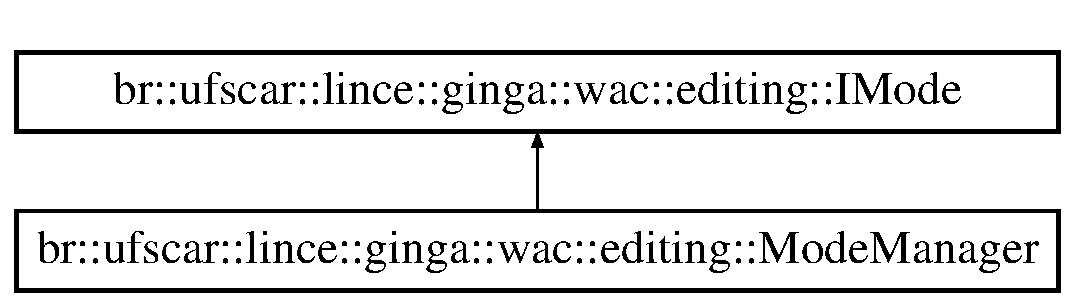
\includegraphics[height=2cm]{classbr_1_1ufscar_1_1lince_1_1ginga_1_1wac_1_1editing_1_1IMode}
\end{center}
\end{figure}
\subsection*{Public Member Functions}
\begin{DoxyCompactItemize}
\item 
virtual bool \hyperlink{classbr_1_1ufscar_1_1lince_1_1ginga_1_1wac_1_1editing_1_1IMode_ab6b8c4de92a5f940f8c726f327f9aa55}{enterClientPresentationMode} ()=0
\begin{DoxyCompactList}\small\item\em Força a entrada no de exibição do cliente. \item\end{DoxyCompactList}\item 
virtual bool \hyperlink{classbr_1_1ufscar_1_1lince_1_1ginga_1_1wac_1_1editing_1_1IMode_a36555fd659519e30880b9d3f4644d257}{exitClientPresentationMode} ()=0
\begin{DoxyCompactList}\small\item\em Força a saida do modo de exibição do cliente. \item\end{DoxyCompactList}\item 
virtual bool \hyperlink{classbr_1_1ufscar_1_1lince_1_1ginga_1_1wac_1_1editing_1_1IMode_a5c0f479717a32e10c4810abdfe4e03d4}{runModeAction} (\hyperlink{classbr_1_1ufscar_1_1lince_1_1ginga_1_1wac_1_1editing_1_1ILinkAction}{ILinkAction} $\ast$linkAction)=0
\begin{DoxyCompactList}\small\item\em Verifica se o determinado elo deve ou não ser disparado dependendo do modo de exibição atual. \item\end{DoxyCompactList}\item 
virtual void \hyperlink{classbr_1_1ufscar_1_1lince_1_1ginga_1_1wac_1_1editing_1_1IMode_a5048bc35fa6ade1b514f79467519b52f}{setScheduler} (\hyperlink{classbr_1_1ufscar_1_1lince_1_1ginga_1_1wac_1_1editing_1_1ISchedulerAdapter}{ISchedulerAdapter} $\ast$scheduler)=0
\begin{DoxyCompactList}\small\item\em Seta a instãncia de Scheculer que será utilizada para matar objetos. \item\end{DoxyCompactList}\end{DoxyCompactItemize}


\subsection{Detailed Description}
Interface que permite a manipulação dos modos de exibição. 

\subsection{Member Function Documentation}
\hypertarget{classbr_1_1ufscar_1_1lince_1_1ginga_1_1wac_1_1editing_1_1IMode_ab6b8c4de92a5f940f8c726f327f9aa55}{
\index{br::ufscar::lince::ginga::wac::editing::IMode@{br::ufscar::lince::ginga::wac::editing::IMode}!enterClientPresentationMode@{enterClientPresentationMode}}
\index{enterClientPresentationMode@{enterClientPresentationMode}!br::ufscar::lince::ginga::wac::editing::IMode@{br::ufscar::lince::ginga::wac::editing::IMode}}
\subsubsection[{enterClientPresentationMode}]{\setlength{\rightskip}{0pt plus 5cm}virtual bool br::ufscar::lince::ginga::wac::editing::IMode::enterClientPresentationMode ()\hspace{0.3cm}{\ttfamily  \mbox{[}pure virtual\mbox{]}}}}
\label{classbr_1_1ufscar_1_1lince_1_1ginga_1_1wac_1_1editing_1_1IMode_ab6b8c4de92a5f940f8c726f327f9aa55}


Força a entrada no de exibição do cliente. 

\begin{DoxyReturn}{Returns}
True se entrou no modo cliente; False se já estava no modo cliente. 
\end{DoxyReturn}


Implemented in \hyperlink{classbr_1_1ufscar_1_1lince_1_1ginga_1_1wac_1_1editing_1_1ModeManager_a5f62cca336317833ac6565a0acc779e6}{br::ufscar::lince::ginga::wac::editing::ModeManager}.

\hypertarget{classbr_1_1ufscar_1_1lince_1_1ginga_1_1wac_1_1editing_1_1IMode_a36555fd659519e30880b9d3f4644d257}{
\index{br::ufscar::lince::ginga::wac::editing::IMode@{br::ufscar::lince::ginga::wac::editing::IMode}!exitClientPresentationMode@{exitClientPresentationMode}}
\index{exitClientPresentationMode@{exitClientPresentationMode}!br::ufscar::lince::ginga::wac::editing::IMode@{br::ufscar::lince::ginga::wac::editing::IMode}}
\subsubsection[{exitClientPresentationMode}]{\setlength{\rightskip}{0pt plus 5cm}virtual bool br::ufscar::lince::ginga::wac::editing::IMode::exitClientPresentationMode ()\hspace{0.3cm}{\ttfamily  \mbox{[}pure virtual\mbox{]}}}}
\label{classbr_1_1ufscar_1_1lince_1_1ginga_1_1wac_1_1editing_1_1IMode_a36555fd659519e30880b9d3f4644d257}


Força a saida do modo de exibição do cliente. 

\begin{DoxyReturn}{Returns}
True se saiu do modo cliente; False se não estava no modo cliente. 
\end{DoxyReturn}


Implemented in \hyperlink{classbr_1_1ufscar_1_1lince_1_1ginga_1_1wac_1_1editing_1_1ModeManager_a7d095b1de1af73c3296f4b6a29c6f08f}{br::ufscar::lince::ginga::wac::editing::ModeManager}.

\hypertarget{classbr_1_1ufscar_1_1lince_1_1ginga_1_1wac_1_1editing_1_1IMode_a5c0f479717a32e10c4810abdfe4e03d4}{
\index{br::ufscar::lince::ginga::wac::editing::IMode@{br::ufscar::lince::ginga::wac::editing::IMode}!runModeAction@{runModeAction}}
\index{runModeAction@{runModeAction}!br::ufscar::lince::ginga::wac::editing::IMode@{br::ufscar::lince::ginga::wac::editing::IMode}}
\subsubsection[{runModeAction}]{\setlength{\rightskip}{0pt plus 5cm}virtual bool br::ufscar::lince::ginga::wac::editing::IMode::runModeAction ({\bf ILinkAction} $\ast$ {\em linkAction})\hspace{0.3cm}{\ttfamily  \mbox{[}pure virtual\mbox{]}}}}
\label{classbr_1_1ufscar_1_1lince_1_1ginga_1_1wac_1_1editing_1_1IMode_a5c0f479717a32e10c4810abdfe4e03d4}


Verifica se o determinado elo deve ou não ser disparado dependendo do modo de exibição atual. 


\begin{DoxyParams}{Parameters}
\item[{\em linkAction}]Elo que será testado quanto a ser ou não disparado. \end{DoxyParams}
\begin{DoxyReturn}{Returns}
True se o elo deve ser disparado; False Caso contrário. 
\end{DoxyReturn}


Implemented in \hyperlink{classbr_1_1ufscar_1_1lince_1_1ginga_1_1wac_1_1editing_1_1ModeManager_a5456384c5ce5e3d7114429e5e28273b8}{br::ufscar::lince::ginga::wac::editing::ModeManager}.

\hypertarget{classbr_1_1ufscar_1_1lince_1_1ginga_1_1wac_1_1editing_1_1IMode_a5048bc35fa6ade1b514f79467519b52f}{
\index{br::ufscar::lince::ginga::wac::editing::IMode@{br::ufscar::lince::ginga::wac::editing::IMode}!setScheduler@{setScheduler}}
\index{setScheduler@{setScheduler}!br::ufscar::lince::ginga::wac::editing::IMode@{br::ufscar::lince::ginga::wac::editing::IMode}}
\subsubsection[{setScheduler}]{\setlength{\rightskip}{0pt plus 5cm}virtual void br::ufscar::lince::ginga::wac::editing::IMode::setScheduler ({\bf ISchedulerAdapter} $\ast$ {\em scheduler})\hspace{0.3cm}{\ttfamily  \mbox{[}pure virtual\mbox{]}}}}
\label{classbr_1_1ufscar_1_1lince_1_1ginga_1_1wac_1_1editing_1_1IMode_a5048bc35fa6ade1b514f79467519b52f}


Seta a instãncia de Scheculer que será utilizada para matar objetos. 


\begin{DoxyParams}{Parameters}
\item[{\em scheduler}]Instância de FormatterScheduler. \end{DoxyParams}


Implemented in \hyperlink{classbr_1_1ufscar_1_1lince_1_1ginga_1_1wac_1_1editing_1_1ModeManager_ac73004e6c04b17ce1673e1fc2a179561}{br::ufscar::lince::ginga::wac::editing::ModeManager}.



The documentation for this class was generated from the following file:\begin{DoxyCompactItemize}
\item 
include/\hyperlink{IMode_8h}{IMode.h}\end{DoxyCompactItemize}

\hypertarget{classbr_1_1ufscar_1_1lince_1_1ginga_1_1wac_1_1editing_1_1IObjectMode}{
\section{br::ufscar::lince::ginga::wac::editing::IObjectMode Class Reference}
\label{classbr_1_1ufscar_1_1lince_1_1ginga_1_1wac_1_1editing_1_1IObjectMode}\index{br::ufscar::lince::ginga::wac::editing::IObjectMode@{br::ufscar::lince::ginga::wac::editing::IObjectMode}}
}


Interface que permite ao módulo Wac-\/Editing Manipular ExecutionObjetcs do módulo Formatter.  




{\ttfamily \#include $<$IObjectMode.h$>$}



\subsection{Detailed Description}
Interface que permite ao módulo Wac-\/Editing Manipular ExecutionObjetcs do módulo Formatter. Através desta interface será possivel ao módulo do Wac-\/Editing obter informações e manipular as instâncias de ExecutionObjetc do módulo Formatter. 

The documentation for this class was generated from the following file:\begin{DoxyCompactItemize}
\item 
include/\hyperlink{IObjectMode_8h}{IObjectMode.h}\end{DoxyCompactItemize}

\hypertarget{classbr_1_1ufscar_1_1lince_1_1ginga_1_1wac_1_1editing_1_1ISchedulerAdapter}{
\section{br::ufscar::lince::ginga::wac::editing::ISchedulerAdapter Class Reference}
\label{classbr_1_1ufscar_1_1lince_1_1ginga_1_1wac_1_1editing_1_1ISchedulerAdapter}\index{br::ufscar::lince::ginga::wac::editing::ISchedulerAdapter@{br::ufscar::lince::ginga::wac::editing::ISchedulerAdapter}}
}


Interface pela qual este módulo envia mensagem a classe Scheduler do módulo Formatter.  




{\ttfamily \#include $<$ISchedulerAdapter.h$>$}

\subsection*{Public Member Functions}
\begin{DoxyCompactItemize}
\item 
virtual \hyperlink{classbr_1_1ufscar_1_1lince_1_1ginga_1_1wac_1_1editing_1_1ISchedulerAdapter_a907bf3b317e57ea1ceb2512d40581070}{$\sim$ISchedulerAdapter} ()
\begin{DoxyCompactList}\small\item\em Destrói a instância de \hyperlink{classbr_1_1ufscar_1_1lince_1_1ginga_1_1wac_1_1editing_1_1ISchedulerAdapter}{ISchedulerAdapter}. \item\end{DoxyCompactList}\item 
virtual void \hyperlink{classbr_1_1ufscar_1_1lince_1_1ginga_1_1wac_1_1editing_1_1ISchedulerAdapter_ac9176e8b3c85cfc3fce05bbcb2285bd1}{stopObject} (\hyperlink{classbr_1_1ufscar_1_1lince_1_1ginga_1_1wac_1_1editing_1_1IObjectMode}{IObjectMode} $\ast$object)=0
\begin{DoxyCompactList}\small\item\em Encerra a apresentação de um determinado objeto. \item\end{DoxyCompactList}\item 
virtual void \hyperlink{classbr_1_1ufscar_1_1lince_1_1ginga_1_1wac_1_1editing_1_1ISchedulerAdapter_a689421a01c70c7915af5a03ee7fc681a}{chanceProperty} (\hyperlink{classbr_1_1ufscar_1_1lince_1_1ginga_1_1wac_1_1editing_1_1IObjectMode}{IObjectMode} $\ast$object, string name, string value)=0
\begin{DoxyCompactList}\small\item\em Permite alterar as propriedades de um determinado objeto em execução. \item\end{DoxyCompactList}\end{DoxyCompactItemize}


\subsection{Detailed Description}
Interface pela qual este módulo envia mensagem a classe Scheduler do módulo Formatter. 

\subsection{Constructor \& Destructor Documentation}
\hypertarget{classbr_1_1ufscar_1_1lince_1_1ginga_1_1wac_1_1editing_1_1ISchedulerAdapter_a907bf3b317e57ea1ceb2512d40581070}{
\index{br::ufscar::lince::ginga::wac::editing::ISchedulerAdapter@{br::ufscar::lince::ginga::wac::editing::ISchedulerAdapter}!$\sim$ISchedulerAdapter@{$\sim$ISchedulerAdapter}}
\index{$\sim$ISchedulerAdapter@{$\sim$ISchedulerAdapter}!br::ufscar::lince::ginga::wac::editing::ISchedulerAdapter@{br::ufscar::lince::ginga::wac::editing::ISchedulerAdapter}}
\subsubsection[{$\sim$ISchedulerAdapter}]{\setlength{\rightskip}{0pt plus 5cm}virtual br::ufscar::lince::ginga::wac::editing::ISchedulerAdapter::$\sim$ISchedulerAdapter ()\hspace{0.3cm}{\ttfamily  \mbox{[}inline, virtual\mbox{]}}}}
\label{classbr_1_1ufscar_1_1lince_1_1ginga_1_1wac_1_1editing_1_1ISchedulerAdapter_a907bf3b317e57ea1ceb2512d40581070}


Destrói a instância de \hyperlink{classbr_1_1ufscar_1_1lince_1_1ginga_1_1wac_1_1editing_1_1ISchedulerAdapter}{ISchedulerAdapter}. 



\subsection{Member Function Documentation}
\hypertarget{classbr_1_1ufscar_1_1lince_1_1ginga_1_1wac_1_1editing_1_1ISchedulerAdapter_a689421a01c70c7915af5a03ee7fc681a}{
\index{br::ufscar::lince::ginga::wac::editing::ISchedulerAdapter@{br::ufscar::lince::ginga::wac::editing::ISchedulerAdapter}!chanceProperty@{chanceProperty}}
\index{chanceProperty@{chanceProperty}!br::ufscar::lince::ginga::wac::editing::ISchedulerAdapter@{br::ufscar::lince::ginga::wac::editing::ISchedulerAdapter}}
\subsubsection[{chanceProperty}]{\setlength{\rightskip}{0pt plus 5cm}virtual void br::ufscar::lince::ginga::wac::editing::ISchedulerAdapter::chanceProperty ({\bf IObjectMode} $\ast$ {\em object}, \/  string {\em name}, \/  string {\em value})\hspace{0.3cm}{\ttfamily  \mbox{[}pure virtual\mbox{]}}}}
\label{classbr_1_1ufscar_1_1lince_1_1ginga_1_1wac_1_1editing_1_1ISchedulerAdapter_a689421a01c70c7915af5a03ee7fc681a}


Permite alterar as propriedades de um determinado objeto em execução. 


\begin{DoxyParams}{Parameters}
\item[{\em object}]Objeto que terá seus propriedades alteradas. \item[{\em name}]Nome da propriedade a ser alterada. \item[{\em value}]Valor a ser setado na propriedade. \end{DoxyParams}
\hypertarget{classbr_1_1ufscar_1_1lince_1_1ginga_1_1wac_1_1editing_1_1ISchedulerAdapter_ac9176e8b3c85cfc3fce05bbcb2285bd1}{
\index{br::ufscar::lince::ginga::wac::editing::ISchedulerAdapter@{br::ufscar::lince::ginga::wac::editing::ISchedulerAdapter}!stopObject@{stopObject}}
\index{stopObject@{stopObject}!br::ufscar::lince::ginga::wac::editing::ISchedulerAdapter@{br::ufscar::lince::ginga::wac::editing::ISchedulerAdapter}}
\subsubsection[{stopObject}]{\setlength{\rightskip}{0pt plus 5cm}virtual void br::ufscar::lince::ginga::wac::editing::ISchedulerAdapter::stopObject ({\bf IObjectMode} $\ast$ {\em object})\hspace{0.3cm}{\ttfamily  \mbox{[}pure virtual\mbox{]}}}}
\label{classbr_1_1ufscar_1_1lince_1_1ginga_1_1wac_1_1editing_1_1ISchedulerAdapter_ac9176e8b3c85cfc3fce05bbcb2285bd1}


Encerra a apresentação de um determinado objeto. 


\begin{DoxyParams}{Parameters}
\item[{\em object}]Objeto que deve ter sua apresentação encerrada. \end{DoxyParams}


The documentation for this class was generated from the following file:\begin{DoxyCompactItemize}
\item 
include/\hyperlink{ISchedulerAdapter_8h}{ISchedulerAdapter.h}\end{DoxyCompactItemize}

\hypertarget{classbr_1_1ufscar_1_1lince_1_1ginga_1_1wac_1_1editing_1_1ModeManager}{
\section{br::ufscar::lince::ginga::wac::editing::ModeManager Class Reference}
\label{classbr_1_1ufscar_1_1lince_1_1ginga_1_1wac_1_1editing_1_1ModeManager}\index{br::ufscar::lince::ginga::wac::editing::ModeManager@{br::ufscar::lince::ginga::wac::editing::ModeManager}}
}


Classe responsável manipular os modos de exibição do cliente e da emissora.  




{\ttfamily \#include $<$ModeManager.h$>$}

Inheritance diagram for br::ufscar::lince::ginga::wac::editing::ModeManager:\begin{figure}[H]
\begin{center}
\leavevmode
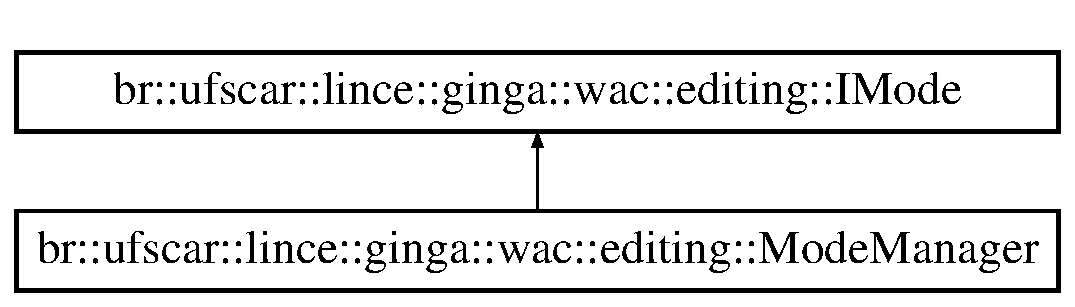
\includegraphics[height=2cm]{classbr_1_1ufscar_1_1lince_1_1ginga_1_1wac_1_1editing_1_1ModeManager}
\end{center}
\end{figure}
\subsection*{Public Member Functions}
\begin{DoxyCompactItemize}
\item 
bool \hyperlink{classbr_1_1ufscar_1_1lince_1_1ginga_1_1wac_1_1editing_1_1ModeManager_a5f62cca336317833ac6565a0acc779e6}{enterClientPresentationMode} ()
\begin{DoxyCompactList}\small\item\em Força a entrada no de exibição do cliente. \item\end{DoxyCompactList}\item 
bool \hyperlink{classbr_1_1ufscar_1_1lince_1_1ginga_1_1wac_1_1editing_1_1ModeManager_a7d095b1de1af73c3296f4b6a29c6f08f}{exitClientPresentationMode} ()
\begin{DoxyCompactList}\small\item\em Força a saida do modo de exibição do cliente. \item\end{DoxyCompactList}\item 
bool \hyperlink{classbr_1_1ufscar_1_1lince_1_1ginga_1_1wac_1_1editing_1_1ModeManager_a5456384c5ce5e3d7114429e5e28273b8}{runModeAction} (\hyperlink{classbr_1_1ufscar_1_1lince_1_1ginga_1_1wac_1_1editing_1_1ILinkAction}{ILinkAction} $\ast$linkAction)
\begin{DoxyCompactList}\small\item\em Verifica se o determinado elo deve ou não ser disparado dependendo do modo de exibição atual. \item\end{DoxyCompactList}\item 
void \hyperlink{classbr_1_1ufscar_1_1lince_1_1ginga_1_1wac_1_1editing_1_1ModeManager_ac73004e6c04b17ce1673e1fc2a179561}{setScheduler} (\hyperlink{classbr_1_1ufscar_1_1lince_1_1ginga_1_1wac_1_1editing_1_1ISchedulerAdapter}{ISchedulerAdapter} $\ast$scheduler)
\begin{DoxyCompactList}\small\item\em Seta a instãncia de Scheculer que será utilizada para matar objetos. \item\end{DoxyCompactList}\end{DoxyCompactItemize}
\subsection*{Static Public Member Functions}
\begin{DoxyCompactItemize}
\item 
static \hyperlink{classbr_1_1ufscar_1_1lince_1_1ginga_1_1wac_1_1editing_1_1IMode}{IMode} $\ast$ \hyperlink{classbr_1_1ufscar_1_1lince_1_1ginga_1_1wac_1_1editing_1_1ModeManager_a1a25cc97eb5724636f205765e03ad785}{getInstance} ()
\begin{DoxyCompactList}\small\item\em Obtém a instância única de \hyperlink{classbr_1_1ufscar_1_1lince_1_1ginga_1_1wac_1_1editing_1_1ModeManager}{ModeManager}. \item\end{DoxyCompactList}\end{DoxyCompactItemize}


\subsection{Detailed Description}
Classe responsável manipular os modos de exibição do cliente e da emissora. Além de ser a responsável por manipular qual o modo atual, também é o responsável por testar os links por liberar ou não a execução dos elos. 

\subsection{Member Function Documentation}
\hypertarget{classbr_1_1ufscar_1_1lince_1_1ginga_1_1wac_1_1editing_1_1ModeManager_a5f62cca336317833ac6565a0acc779e6}{
\index{br::ufscar::lince::ginga::wac::editing::ModeManager@{br::ufscar::lince::ginga::wac::editing::ModeManager}!enterClientPresentationMode@{enterClientPresentationMode}}
\index{enterClientPresentationMode@{enterClientPresentationMode}!br::ufscar::lince::ginga::wac::editing::ModeManager@{br::ufscar::lince::ginga::wac::editing::ModeManager}}
\subsubsection[{enterClientPresentationMode}]{\setlength{\rightskip}{0pt plus 5cm}bool br::ufscar::lince::ginga::wac::editing::ModeManager::enterClientPresentationMode ()\hspace{0.3cm}{\ttfamily  \mbox{[}virtual\mbox{]}}}}
\label{classbr_1_1ufscar_1_1lince_1_1ginga_1_1wac_1_1editing_1_1ModeManager_a5f62cca336317833ac6565a0acc779e6}


Força a entrada no de exibição do cliente. 

\begin{DoxyReturn}{Returns}
True se entrou no modo cliente; False se já estava no modo cliente. 
\end{DoxyReturn}


Implements \hyperlink{classbr_1_1ufscar_1_1lince_1_1ginga_1_1wac_1_1editing_1_1IMode_ab6b8c4de92a5f940f8c726f327f9aa55}{br::ufscar::lince::ginga::wac::editing::IMode}.

\hypertarget{classbr_1_1ufscar_1_1lince_1_1ginga_1_1wac_1_1editing_1_1ModeManager_a7d095b1de1af73c3296f4b6a29c6f08f}{
\index{br::ufscar::lince::ginga::wac::editing::ModeManager@{br::ufscar::lince::ginga::wac::editing::ModeManager}!exitClientPresentationMode@{exitClientPresentationMode}}
\index{exitClientPresentationMode@{exitClientPresentationMode}!br::ufscar::lince::ginga::wac::editing::ModeManager@{br::ufscar::lince::ginga::wac::editing::ModeManager}}
\subsubsection[{exitClientPresentationMode}]{\setlength{\rightskip}{0pt plus 5cm}bool br::ufscar::lince::ginga::wac::editing::ModeManager::exitClientPresentationMode ()\hspace{0.3cm}{\ttfamily  \mbox{[}virtual\mbox{]}}}}
\label{classbr_1_1ufscar_1_1lince_1_1ginga_1_1wac_1_1editing_1_1ModeManager_a7d095b1de1af73c3296f4b6a29c6f08f}


Força a saida do modo de exibição do cliente. 

\begin{DoxyReturn}{Returns}
True se saiu do modo cliente; False se não estava no modo cliente. 
\end{DoxyReturn}


Implements \hyperlink{classbr_1_1ufscar_1_1lince_1_1ginga_1_1wac_1_1editing_1_1IMode_a36555fd659519e30880b9d3f4644d257}{br::ufscar::lince::ginga::wac::editing::IMode}.

\hypertarget{classbr_1_1ufscar_1_1lince_1_1ginga_1_1wac_1_1editing_1_1ModeManager_a1a25cc97eb5724636f205765e03ad785}{
\index{br::ufscar::lince::ginga::wac::editing::ModeManager@{br::ufscar::lince::ginga::wac::editing::ModeManager}!getInstance@{getInstance}}
\index{getInstance@{getInstance}!br::ufscar::lince::ginga::wac::editing::ModeManager@{br::ufscar::lince::ginga::wac::editing::ModeManager}}
\subsubsection[{getInstance}]{\setlength{\rightskip}{0pt plus 5cm}static {\bf IMode}$\ast$ br::ufscar::lince::ginga::wac::editing::ModeManager::getInstance ()\hspace{0.3cm}{\ttfamily  \mbox{[}static\mbox{]}}}}
\label{classbr_1_1ufscar_1_1lince_1_1ginga_1_1wac_1_1editing_1_1ModeManager_a1a25cc97eb5724636f205765e03ad785}


Obtém a instância única de \hyperlink{classbr_1_1ufscar_1_1lince_1_1ginga_1_1wac_1_1editing_1_1ModeManager}{ModeManager}. 

\begin{DoxyReturn}{Returns}
Instância única de \hyperlink{classbr_1_1ufscar_1_1lince_1_1ginga_1_1wac_1_1editing_1_1ModeManager}{ModeManager}. 
\end{DoxyReturn}
\hypertarget{classbr_1_1ufscar_1_1lince_1_1ginga_1_1wac_1_1editing_1_1ModeManager_a5456384c5ce5e3d7114429e5e28273b8}{
\index{br::ufscar::lince::ginga::wac::editing::ModeManager@{br::ufscar::lince::ginga::wac::editing::ModeManager}!runModeAction@{runModeAction}}
\index{runModeAction@{runModeAction}!br::ufscar::lince::ginga::wac::editing::ModeManager@{br::ufscar::lince::ginga::wac::editing::ModeManager}}
\subsubsection[{runModeAction}]{\setlength{\rightskip}{0pt plus 5cm}bool br::ufscar::lince::ginga::wac::editing::ModeManager::runModeAction ({\bf ILinkAction} $\ast$ {\em linkAction})\hspace{0.3cm}{\ttfamily  \mbox{[}virtual\mbox{]}}}}
\label{classbr_1_1ufscar_1_1lince_1_1ginga_1_1wac_1_1editing_1_1ModeManager_a5456384c5ce5e3d7114429e5e28273b8}


Verifica se o determinado elo deve ou não ser disparado dependendo do modo de exibição atual. 


\begin{DoxyParams}{Parameters}
\item[{\em linkAction}]Elo que será testado quanto a ser ou não disparado. \end{DoxyParams}
\begin{DoxyReturn}{Returns}
True se o elo deve ser disparado; False Caso contrário. 
\end{DoxyReturn}


Implements \hyperlink{classbr_1_1ufscar_1_1lince_1_1ginga_1_1wac_1_1editing_1_1IMode_a5c0f479717a32e10c4810abdfe4e03d4}{br::ufscar::lince::ginga::wac::editing::IMode}.

\hypertarget{classbr_1_1ufscar_1_1lince_1_1ginga_1_1wac_1_1editing_1_1ModeManager_ac73004e6c04b17ce1673e1fc2a179561}{
\index{br::ufscar::lince::ginga::wac::editing::ModeManager@{br::ufscar::lince::ginga::wac::editing::ModeManager}!setScheduler@{setScheduler}}
\index{setScheduler@{setScheduler}!br::ufscar::lince::ginga::wac::editing::ModeManager@{br::ufscar::lince::ginga::wac::editing::ModeManager}}
\subsubsection[{setScheduler}]{\setlength{\rightskip}{0pt plus 5cm}void br::ufscar::lince::ginga::wac::editing::ModeManager::setScheduler ({\bf ISchedulerAdapter} $\ast$ {\em scheduler})\hspace{0.3cm}{\ttfamily  \mbox{[}virtual\mbox{]}}}}
\label{classbr_1_1ufscar_1_1lince_1_1ginga_1_1wac_1_1editing_1_1ModeManager_ac73004e6c04b17ce1673e1fc2a179561}


Seta a instãncia de Scheculer que será utilizada para matar objetos. 


\begin{DoxyParams}{Parameters}
\item[{\em scheduler}]Instância de FormatterScheduler. \end{DoxyParams}


Implements \hyperlink{classbr_1_1ufscar_1_1lince_1_1ginga_1_1wac_1_1editing_1_1IMode_a5048bc35fa6ade1b514f79467519b52f}{br::ufscar::lince::ginga::wac::editing::IMode}.



The documentation for this class was generated from the following file:\begin{DoxyCompactItemize}
\item 
include/\hyperlink{ModeManager_8h}{ModeManager.h}\end{DoxyCompactItemize}

\chapter{File Documentation}
\hypertarget{ClientEditingManager_8h}{
\section{include/ClientEditingManager.h File Reference}
\label{ClientEditingManager_8h}\index{include/ClientEditingManager.h@{include/ClientEditingManager.h}}
}
{\ttfamily \#include $<$list$>$}\par
{\ttfamily \#include $<$string$>$}\par
{\ttfamily \#include $<$cstdlib$>$}\par
{\ttfamily \#include $<$map$>$}\par
{\ttfamily \#include \char`\"{}ncl/generator/NclGenerator.h\char`\"{}}\par
{\ttfamily \#include \char`\"{}ncl/generator/NclDocumentGenerator.h\char`\"{}}\par
{\ttfamily \#include \char`\"{}ncl/generator/NclFileGenerator.h\char`\"{}}\par
{\ttfamily \#include \char`\"{}util/functions.h\char`\"{}}\par
{\ttfamily \#include \char`\"{}IClientEditing.h\char`\"{}}\par
{\ttfamily \#include \char`\"{}ncl/components/Node.h\char`\"{}}\par
{\ttfamily \#include \char`\"{}ncl/interfaces/InterfacePoint.h\char`\"{}}\par
{\ttfamily \#include \char`\"{}ncl/switches/Rule.h\char`\"{}}\par
{\ttfamily \#include \char`\"{}ncl/descriptor/GenericDescriptor.h\char`\"{}}\par
{\ttfamily \#include \char`\"{}ncl/link/Link.h\char`\"{}}\par
{\ttfamily \#include \char`\"{}ncl/connectors/Connector.h\char`\"{}}\par
{\ttfamily \#include \char`\"{}ncl/layout/LayoutRegion.h\char`\"{}}\par
{\ttfamily \#include \char`\"{}ncl/transition/Transition.h\char`\"{}}\par
{\ttfamily \#include \char`\"{}ncl/NclDocument.h\char`\"{}}\par
{\ttfamily \#include \char`\"{}ncl/components/ContextNode.h\char`\"{}}\par
{\ttfamily \#include \char`\"{}ncl/components/CompositeNode.h\char`\"{}}\par
{\ttfamily \#include \char`\"{}ncl/components/ContentNode.h\char`\"{}}\par
{\ttfamily \#include \char`\"{}ncl/components/NodeEntity.h\char`\"{}}\par
{\ttfamily \#include \char`\"{}ncl/interfaces/Anchor.h\char`\"{}}\par
{\ttfamily \#include \char`\"{}ncl/interfaces/PropertyAnchor.h\char`\"{}}\par
{\ttfamily \#include \char`\"{}ncl/interfaces/Port.h\char`\"{}}\par
{\ttfamily \#include \char`\"{}ncl/interfaces/SwitchPort.h\char`\"{}}\par
{\ttfamily \#include \char`\"{}ncl/link/Bind.h\char`\"{}}\par
{\ttfamily \#include \char`\"{}ncl/link/CausalLink.h\char`\"{}}\par
{\ttfamily \#include \char`\"{}ncl/link/LinkComposition.h\char`\"{}}\par
{\ttfamily \#include \char`\"{}ncl/connectors/EventUtil.h\char`\"{}}\par
{\ttfamily \#include \char`\"{}ncl/connectors/SimpleAction.h\char`\"{}}\par
{\ttfamily \#include \char`\"{}ncl/reuse/ReferNode.h\char`\"{}}\par
{\ttfamily \#include \char`\"{}ncl/Base.h\char`\"{}}\par
{\ttfamily \#include \char`\"{}ncl/connectors/ConnectorBase.h\char`\"{}}\par
{\ttfamily \#include \char`\"{}ncl/descriptor/DescriptorBase.h\char`\"{}}\par
{\ttfamily \#include \char`\"{}ncl/layout/RegionBase.h\char`\"{}}\par
{\ttfamily \#include \char`\"{}ncl/switches/RuleBase.h\char`\"{}}\par
{\ttfamily \#include \char`\"{}ncl/transition/TransitionBase.h\char`\"{}}\par
{\ttfamily \#include \char`\"{}IObjectMode.h\char`\"{}}\par
{\ttfamily \#include $<$ginga/linceutil/LoggerUtil.h$>$}\par
\subsection*{Data Structures}
\begin{DoxyCompactItemize}
\item 
class \hyperlink{classbr_1_1ufscar_1_1lince_1_1ginga_1_1wac_1_1editing_1_1ClientEditingManager}{br::ufscar::lince::ginga::wac::editing::ClientEditingManager}
\begin{DoxyCompactList}\small\item\em Permite a aplicações desenvolvidas pelo usuário realizar anotações e edições ao vivo em um documento NCL Esta classe basicamente facilita a criação de aplicações de anotação e edição ao vivo do lado cliente, pois faz parte das tarefas necessárias para aplicações deste tipo, além de permitir retroceder de alterações erroneas e fazer um log das alterações. \item\end{DoxyCompactList}\end{DoxyCompactItemize}
\subsection*{Namespaces}
\begin{DoxyCompactItemize}
\item 
namespace \hyperlink{namespacebr}{br}
\item 
namespace \hyperlink{namespacebr_1_1ufscar}{br::ufscar}
\item 
namespace \hyperlink{namespacebr_1_1ufscar_1_1lince}{br::ufscar::lince}
\item 
namespace \hyperlink{namespacebr_1_1ufscar_1_1lince_1_1ginga}{br::ufscar::lince::ginga}
\item 
namespace \hyperlink{namespacebr_1_1ufscar_1_1lince_1_1ginga_1_1wac}{br::ufscar::lince::ginga::wac}
\item 
namespace \hyperlink{namespacebr_1_1ufscar_1_1lince_1_1ginga_1_1wac_1_1editing}{br::ufscar::lince::ginga::wac::editing}
\end{DoxyCompactItemize}


\subsection{Detailed Description}
\begin{DoxyAuthor}{Author}
Caio Viel 
\end{DoxyAuthor}
\begin{DoxyDate}{Date}
29-\/01-\/10 
\end{DoxyDate}

\hypertarget{EditingCommand_8h}{
\section{include/EditingCommand.h File Reference}
\label{EditingCommand_8h}\index{include/EditingCommand.h@{include/EditingCommand.h}}
}
{\ttfamily \#include $<$string$>$}\par
{\ttfamily \#include $<$cstdlib$>$}\par
{\ttfamily \#include \char`\"{}ncl/components/Node.h\char`\"{}}\par
{\ttfamily \#include \char`\"{}ncl/interfaces/InterfacePoint.h\char`\"{}}\par
{\ttfamily \#include \char`\"{}ncl/switches/Rule.h\char`\"{}}\par
{\ttfamily \#include \char`\"{}ncl/descriptor/GenericDescriptor.h\char`\"{}}\par
{\ttfamily \#include \char`\"{}ncl/link/Link.h\char`\"{}}\par
{\ttfamily \#include \char`\"{}ncl/connectors/Connector.h\char`\"{}}\par
{\ttfamily \#include \char`\"{}ncl/layout/LayoutRegion.h\char`\"{}}\par
{\ttfamily \#include \char`\"{}ncl/transition/Transition.h\char`\"{}}\par
\subsection*{Data Structures}
\begin{DoxyCompactItemize}
\item 
class \hyperlink{classbr_1_1ufscar_1_1lince_1_1ginga_1_1wac_1_1editing_1_1EditingCommand}{br::ufscar::lince::ginga::wac::editing::EditingCommand}
\begin{DoxyCompactList}\small\item\em Classe que encapsula comandos de edição ao vivo do usuário. \item\end{DoxyCompactList}\end{DoxyCompactItemize}
\subsection*{Namespaces}
\begin{DoxyCompactItemize}
\item 
namespace \hyperlink{namespacebr}{br}
\item 
namespace \hyperlink{namespacebr_1_1ufscar}{br::ufscar}
\item 
namespace \hyperlink{namespacebr_1_1ufscar_1_1lince}{br::ufscar::lince}
\item 
namespace \hyperlink{namespacebr_1_1ufscar_1_1lince_1_1ginga}{br::ufscar::lince::ginga}
\item 
namespace \hyperlink{namespacebr_1_1ufscar_1_1lince_1_1ginga_1_1wac}{br::ufscar::lince::ginga::wac}
\item 
namespace \hyperlink{namespacebr_1_1ufscar_1_1lince_1_1ginga_1_1wac_1_1editing}{br::ufscar::lince::ginga::wac::editing}
\end{DoxyCompactItemize}


\subsection{Detailed Description}
\begin{DoxyAuthor}{Author}
Caio Viel 
\end{DoxyAuthor}
\begin{DoxyDate}{Date}
29-\/01-\/10 
\end{DoxyDate}

\hypertarget{IClientEditing_8h}{
\section{include/IClientEditing.h File Reference}
\label{IClientEditing_8h}\index{include/IClientEditing.h@{include/IClientEditing.h}}
}
{\ttfamily \#include \char`\"{}ncl/components/Node.h\char`\"{}}\par
{\ttfamily \#include \char`\"{}ncl/interfaces/InterfacePoint.h\char`\"{}}\par
{\ttfamily \#include \char`\"{}ncl/switches/Rule.h\char`\"{}}\par
{\ttfamily \#include \char`\"{}ncl/descriptor/GenericDescriptor.h\char`\"{}}\par
{\ttfamily \#include \char`\"{}ncl/link/Link.h\char`\"{}}\par
{\ttfamily \#include \char`\"{}ncl/connectors/Connector.h\char`\"{}}\par
{\ttfamily \#include \char`\"{}ncl/layout/LayoutRegion.h\char`\"{}}\par
{\ttfamily \#include \char`\"{}ncl/transition/Transition.h\char`\"{}}\par
{\ttfamily \#include \char`\"{}ncl/NclDocument.h\char`\"{}}\par
{\ttfamily \#include $<$cstdlib$>$}\par
{\ttfamily \#include $<$string$>$}\par
\subsection*{Data Structures}
\begin{DoxyCompactItemize}
\item 
class \hyperlink{classbr_1_1ufscar_1_1lince_1_1ginga_1_1wac_1_1editing_1_1IClientEditing}{br::ufscar::lince::ginga::wac::editing::IClientEditing}
\begin{DoxyCompactList}\small\item\em Interface utilizada pelas aplicações do cliente para utilizar os serviçõs do módulo ClientEditig. \item\end{DoxyCompactList}\end{DoxyCompactItemize}
\subsection*{Namespaces}
\begin{DoxyCompactItemize}
\item 
namespace \hyperlink{namespacebr}{br}
\item 
namespace \hyperlink{namespacebr_1_1ufscar}{br::ufscar}
\item 
namespace \hyperlink{namespacebr_1_1ufscar_1_1lince}{br::ufscar::lince}
\item 
namespace \hyperlink{namespacebr_1_1ufscar_1_1lince_1_1ginga}{br::ufscar::lince::ginga}
\item 
namespace \hyperlink{namespacebr_1_1ufscar_1_1lince_1_1ginga_1_1wac}{br::ufscar::lince::ginga::wac}
\item 
namespace \hyperlink{namespacebr_1_1ufscar_1_1lince_1_1ginga_1_1wac_1_1editing}{br::ufscar::lince::ginga::wac::editing}
\end{DoxyCompactItemize}


\subsection{Detailed Description}
\begin{DoxyAuthor}{Author}
Caio Viel 
\end{DoxyAuthor}
\begin{DoxyDate}{Date}
29-\/01-\/10 
\end{DoxyDate}

\hypertarget{IFormatterAdapter_8h}{
\section{include/IFormatterAdapter.h File Reference}
\label{IFormatterAdapter_8h}\index{include/IFormatterAdapter.h@{include/IFormatterAdapter.h}}
}
{\ttfamily \#include \char`\"{}ncl/components/ContextNode.h\char`\"{}}\par
{\ttfamily \#include \char`\"{}ncl/components/CompositeNode.h\char`\"{}}\par
{\ttfamily \#include \char`\"{}ncl/components/ContentNode.h\char`\"{}}\par
{\ttfamily \#include \char`\"{}ncl/components/Node.h\char`\"{}}\par
{\ttfamily \#include \char`\"{}ncl/components/NodeEntity.h\char`\"{}}\par
{\ttfamily \#include \char`\"{}ncl/interfaces/Anchor.h\char`\"{}}\par
{\ttfamily \#include \char`\"{}ncl/interfaces/PropertyAnchor.h\char`\"{}}\par
{\ttfamily \#include \char`\"{}ncl/interfaces/Port.h\char`\"{}}\par
{\ttfamily \#include \char`\"{}ncl/interfaces/SwitchPort.h\char`\"{}}\par
{\ttfamily \#include \char`\"{}ncl/interfaces/InterfacePoint.h\char`\"{}}\par
{\ttfamily \#include \char`\"{}ncl/switches/Rule.h\char`\"{}}\par
{\ttfamily \#include \char`\"{}ncl/descriptor/GenericDescriptor.h\char`\"{}}\par
{\ttfamily \#include \char`\"{}ncl/link/Bind.h\char`\"{}}\par
{\ttfamily \#include \char`\"{}ncl/link/CausalLink.h\char`\"{}}\par
{\ttfamily \#include \char`\"{}ncl/link/Link.h\char`\"{}}\par
{\ttfamily \#include \char`\"{}ncl/link/LinkComposition.h\char`\"{}}\par
{\ttfamily \#include \char`\"{}ncl/connectors/EventUtil.h\char`\"{}}\par
{\ttfamily \#include \char`\"{}ncl/connectors/SimpleAction.h\char`\"{}}\par
{\ttfamily \#include \char`\"{}ncl/connectors/Connector.h\char`\"{}}\par
{\ttfamily \#include \char`\"{}ncl/layout/LayoutRegion.h\char`\"{}}\par
{\ttfamily \#include \char`\"{}ncl/reuse/ReferNode.h\char`\"{}}\par
{\ttfamily \#include \char`\"{}util/functions.h\char`\"{}}\par
{\ttfamily \#include \char`\"{}ncl/Base.h\char`\"{}}\par
{\ttfamily \#include \char`\"{}ncl/connectors/ConnectorBase.h\char`\"{}}\par
{\ttfamily \#include \char`\"{}ncl/descriptor/DescriptorBase.h\char`\"{}}\par
{\ttfamily \#include \char`\"{}ncl/layout/RegionBase.h\char`\"{}}\par
{\ttfamily \#include \char`\"{}ncl/switches/RuleBase.h\char`\"{}}\par
{\ttfamily \#include \char`\"{}ncl/transition/Transition.h\char`\"{}}\par
{\ttfamily \#include \char`\"{}ncl/transition/TransitionBase.h\char`\"{}}\par
{\ttfamily \#include \char`\"{}ncl/NclDocument.h\char`\"{}}\par
{\ttfamily \#include $<$cstdlib$>$}\par
{\ttfamily \#include $<$string$>$}\par
\subsection*{Data Structures}
\begin{DoxyCompactItemize}
\item 
class \hyperlink{classbr_1_1ufscar_1_1lince_1_1ginga_1_1wac_1_1editing_1_1IFormatterAdapter}{br::ufscar::lince::ginga::wac::editing::IFormatterAdapter}
\begin{DoxyCompactList}\small\item\em Interface que permite que as classes do módulo Wac-\/Editing enviem mensagem a classe Formatter do módulo Formatter. \item\end{DoxyCompactList}\end{DoxyCompactItemize}
\subsection*{Namespaces}
\begin{DoxyCompactItemize}
\item 
namespace \hyperlink{namespacebr}{br}
\item 
namespace \hyperlink{namespacebr_1_1ufscar}{br::ufscar}
\item 
namespace \hyperlink{namespacebr_1_1ufscar_1_1lince}{br::ufscar::lince}
\item 
namespace \hyperlink{namespacebr_1_1ufscar_1_1lince_1_1ginga}{br::ufscar::lince::ginga}
\item 
namespace \hyperlink{namespacebr_1_1ufscar_1_1lince_1_1ginga_1_1wac}{br::ufscar::lince::ginga::wac}
\item 
namespace \hyperlink{namespacebr_1_1ufscar_1_1lince_1_1ginga_1_1wac_1_1editing}{br::ufscar::lince::ginga::wac::editing}
\end{DoxyCompactItemize}


\subsection{Detailed Description}
\begin{DoxyAuthor}{Author}
Caio Viel 
\end{DoxyAuthor}
\begin{DoxyDate}{Date}
29-\/01-\/10 
\end{DoxyDate}

\hypertarget{ILinkAction_8h}{
\section{include/ILinkAction.h File Reference}
\label{ILinkAction_8h}\index{include/ILinkAction.h@{include/ILinkAction.h}}
}
{\ttfamily \#include \char`\"{}IObjectMode.h\char`\"{}}\par
\subsection*{Data Structures}
\begin{DoxyCompactItemize}
\item 
class \hyperlink{classbr_1_1ufscar_1_1lince_1_1ginga_1_1wac_1_1editing_1_1ILinkAction}{br::ufscar::lince::ginga::wac::editing::ILinkAction}
\begin{DoxyCompactList}\small\item\em Interface pela qual é possivel obter informações sobre os links do módulo Formatter. \item\end{DoxyCompactList}\end{DoxyCompactItemize}
\subsection*{Namespaces}
\begin{DoxyCompactItemize}
\item 
namespace \hyperlink{namespacebr}{br}
\item 
namespace \hyperlink{namespacebr_1_1ufscar}{br::ufscar}
\item 
namespace \hyperlink{namespacebr_1_1ufscar_1_1lince}{br::ufscar::lince}
\item 
namespace \hyperlink{namespacebr_1_1ufscar_1_1lince_1_1ginga}{br::ufscar::lince::ginga}
\item 
namespace \hyperlink{namespacebr_1_1ufscar_1_1lince_1_1ginga_1_1wac}{br::ufscar::lince::ginga::wac}
\item 
namespace \hyperlink{namespacebr_1_1ufscar_1_1lince_1_1ginga_1_1wac_1_1editing}{br::ufscar::lince::ginga::wac::editing}
\end{DoxyCompactItemize}


\subsection{Detailed Description}
\begin{DoxyAuthor}{Author}
Caio Viel 
\end{DoxyAuthor}
\begin{DoxyDate}{Date}
29-\/01-\/10 
\end{DoxyDate}

\hypertarget{IMode_8h}{
\section{include/IMode.h File Reference}
\label{IMode_8h}\index{include/IMode.h@{include/IMode.h}}
}
{\ttfamily \#include \char`\"{}ISchedulerAdapter.h\char`\"{}}\par
{\ttfamily \#include \char`\"{}ILinkAction.h\char`\"{}}\par
{\ttfamily \#include \char`\"{}IObjectMode.h\char`\"{}}\par
\subsection*{Data Structures}
\begin{DoxyCompactItemize}
\item 
class \hyperlink{classbr_1_1ufscar_1_1lince_1_1ginga_1_1wac_1_1editing_1_1IMode}{br::ufscar::lince::ginga::wac::editing::IMode}
\begin{DoxyCompactList}\small\item\em Interface que permite a manipulação dos modos de exibição. \item\end{DoxyCompactList}\end{DoxyCompactItemize}
\subsection*{Namespaces}
\begin{DoxyCompactItemize}
\item 
namespace \hyperlink{namespacebr}{br}
\item 
namespace \hyperlink{namespacebr_1_1ufscar}{br::ufscar}
\item 
namespace \hyperlink{namespacebr_1_1ufscar_1_1lince}{br::ufscar::lince}
\item 
namespace \hyperlink{namespacebr_1_1ufscar_1_1lince_1_1ginga}{br::ufscar::lince::ginga}
\item 
namespace \hyperlink{namespacebr_1_1ufscar_1_1lince_1_1ginga_1_1wac}{br::ufscar::lince::ginga::wac}
\item 
namespace \hyperlink{namespacebr_1_1ufscar_1_1lince_1_1ginga_1_1wac_1_1editing}{br::ufscar::lince::ginga::wac::editing}
\end{DoxyCompactItemize}


\subsection{Detailed Description}
\begin{DoxyAuthor}{Author}
Caio Viel 
\end{DoxyAuthor}
\begin{DoxyDate}{Date}
29-\/01-\/10 
\end{DoxyDate}

\hypertarget{IObjectMode_8h}{
\section{include/IObjectMode.h File Reference}
\label{IObjectMode_8h}\index{include/IObjectMode.h@{include/IObjectMode.h}}
}
{\ttfamily \#include \char`\"{}IObjectMode.h\char`\"{}}\par
{\ttfamily \#include $<$cstdlib$>$}\par
{\ttfamily \#include $<$string$>$}\par
\subsection*{Data Structures}
\begin{DoxyCompactItemize}
\item 
class \hyperlink{classbr_1_1ufscar_1_1lince_1_1ginga_1_1wac_1_1editing_1_1IObjectMode}{br::ufscar::lince::ginga::wac::editing::IObjectMode}
\begin{DoxyCompactList}\small\item\em Interface que permite ao módulo Wac-\/Editing Manipular ExecutionObjetcs do módulo Formatter. \item\end{DoxyCompactList}\end{DoxyCompactItemize}
\subsection*{Namespaces}
\begin{DoxyCompactItemize}
\item 
namespace \hyperlink{namespacebr}{br}
\item 
namespace \hyperlink{namespacebr_1_1ufscar}{br::ufscar}
\item 
namespace \hyperlink{namespacebr_1_1ufscar_1_1lince}{br::ufscar::lince}
\item 
namespace \hyperlink{namespacebr_1_1ufscar_1_1lince_1_1ginga}{br::ufscar::lince::ginga}
\item 
namespace \hyperlink{namespacebr_1_1ufscar_1_1lince_1_1ginga_1_1wac}{br::ufscar::lince::ginga::wac}
\item 
namespace \hyperlink{namespacebr_1_1ufscar_1_1lince_1_1ginga_1_1wac_1_1editing}{br::ufscar::lince::ginga::wac::editing}
\end{DoxyCompactItemize}


\subsection{Detailed Description}
\begin{DoxyAuthor}{Author}
Caio Viel 
\end{DoxyAuthor}
\begin{DoxyDate}{Date}
29-\/01-\/10 
\end{DoxyDate}

\hypertarget{ISchedulerAdapter_8h}{
\section{include/ISchedulerAdapter.h File Reference}
\label{ISchedulerAdapter_8h}\index{include/ISchedulerAdapter.h@{include/ISchedulerAdapter.h}}
}
{\ttfamily \#include \char`\"{}IObjectMode.h\char`\"{}}\par
{\ttfamily \#include $<$cstdlib$>$}\par
{\ttfamily \#include $<$string$>$}\par
\subsection*{Data Structures}
\begin{DoxyCompactItemize}
\item 
class \hyperlink{classbr_1_1ufscar_1_1lince_1_1ginga_1_1wac_1_1editing_1_1ISchedulerAdapter}{br::ufscar::lince::ginga::wac::editing::ISchedulerAdapter}
\begin{DoxyCompactList}\small\item\em Interface pela qual este módulo envia mensagem a classe Scheduler do módulo Formatter. \item\end{DoxyCompactList}\end{DoxyCompactItemize}
\subsection*{Namespaces}
\begin{DoxyCompactItemize}
\item 
namespace \hyperlink{namespacebr}{br}
\item 
namespace \hyperlink{namespacebr_1_1ufscar}{br::ufscar}
\item 
namespace \hyperlink{namespacebr_1_1ufscar_1_1lince}{br::ufscar::lince}
\item 
namespace \hyperlink{namespacebr_1_1ufscar_1_1lince_1_1ginga}{br::ufscar::lince::ginga}
\item 
namespace \hyperlink{namespacebr_1_1ufscar_1_1lince_1_1ginga_1_1wac}{br::ufscar::lince::ginga::wac}
\item 
namespace \hyperlink{namespacebr_1_1ufscar_1_1lince_1_1ginga_1_1wac_1_1editing}{br::ufscar::lince::ginga::wac::editing}
\end{DoxyCompactItemize}


\subsection{Detailed Description}
\begin{DoxyAuthor}{Author}
Caio Viel 
\end{DoxyAuthor}
\begin{DoxyDate}{Date}
29-\/01-\/10 
\end{DoxyDate}

\hypertarget{ModeManager_8h}{
\section{include/ModeManager.h File Reference}
\label{ModeManager_8h}\index{include/ModeManager.h@{include/ModeManager.h}}
}
{\ttfamily \#include \char`\"{}IMode.h\char`\"{}}\par
{\ttfamily \#include \char`\"{}ISchedulerAdapter.h\char`\"{}}\par
{\ttfamily \#include \char`\"{}ILinkAction.h\char`\"{}}\par
{\ttfamily \#include \char`\"{}IFormatterAdapter.h\char`\"{}}\par
{\ttfamily \#include $<$list$>$}\par
{\ttfamily \#include $<$string$>$}\par
{\ttfamily \#include $<$cstdlib$>$}\par
{\ttfamily \#include $<$map$>$}\par
{\ttfamily \#include \char`\"{}ncl/generator/NclGenerator.h\char`\"{}}\par
{\ttfamily \#include \char`\"{}ncl/generator/NclDocumentGenerator.h\char`\"{}}\par
{\ttfamily \#include \char`\"{}ncl/generator/NclFileGenerator.h\char`\"{}}\par
{\ttfamily \#include \char`\"{}util/functions.h\char`\"{}}\par
{\ttfamily \#include \char`\"{}IClientEditing.h\char`\"{}}\par
{\ttfamily \#include \char`\"{}EditingCommand.h\char`\"{}}\par
{\ttfamily \#include $<$ginga/linceutil/LoggerUtil.h$>$}\par
{\ttfamily \#include $<$vector$>$}\par
\subsection*{Data Structures}
\begin{DoxyCompactItemize}
\item 
class \hyperlink{classbr_1_1ufscar_1_1lince_1_1ginga_1_1wac_1_1editing_1_1ModeManager}{br::ufscar::lince::ginga::wac::editing::ModeManager}
\begin{DoxyCompactList}\small\item\em Classe responsável manipular os modos de exibição do cliente e da emissora. \item\end{DoxyCompactList}\end{DoxyCompactItemize}
\subsection*{Namespaces}
\begin{DoxyCompactItemize}
\item 
namespace \hyperlink{namespacebr}{br}
\item 
namespace \hyperlink{namespacebr_1_1ufscar}{br::ufscar}
\item 
namespace \hyperlink{namespacebr_1_1ufscar_1_1lince}{br::ufscar::lince}
\item 
namespace \hyperlink{namespacebr_1_1ufscar_1_1lince_1_1ginga}{br::ufscar::lince::ginga}
\item 
namespace \hyperlink{namespacebr_1_1ufscar_1_1lince_1_1ginga_1_1wac}{br::ufscar::lince::ginga::wac}
\item 
namespace \hyperlink{namespacebr_1_1ufscar_1_1lince_1_1ginga_1_1wac_1_1editing}{br::ufscar::lince::ginga::wac::editing}
\end{DoxyCompactItemize}


\subsection{Detailed Description}
\begin{DoxyAuthor}{Author}
Caio Viel 
\end{DoxyAuthor}
\begin{DoxyDate}{Date}
29-\/01-\/10 
\end{DoxyDate}

\printindex
\end{document}
